% LaTeX source for ``Think DSP: Digital Signal Processing for Programmers''
% Copyright 2014  Allen B. Downey.

% License: Creative Commons Attribution-NonCommercial 3.0 Unported License.
% http://creativecommons.org/licenses/by-nc/3.0/
%

\documentclass[12pt]{book}
\usepackage[width=5.5in,height=8.5in,
  hmarginratio=3:2,vmarginratio=1:1]{geometry}

% for some of these packages, you might have to install
% texlive-latex-extra (in Ubuntu)

\usepackage[T1]{fontenc}
\usepackage{textcomp}
\usepackage{mathpazo}
\usepackage{url}
\usepackage{graphicx}
\usepackage{subfig}
\usepackage{amsmath}
\usepackage{amsthm}
\usepackage{makeidx}
\usepackage{setspace}
\usepackage{hevea}                           
\usepackage{upquote}
\usepackage{fancyhdr}
\usepackage[bookmarks]{hyperref}

\title{Think DSP}
\author{Allen B. Downey}

\newcommand{\thetitle}{Think DSP: Digital Signal Processing in Python}
\newcommand{\theversion}{0.9.5}

% these styles get translated in CSS for the HTML version
\newstyle{a:link}{color:black;}
\newstyle{p+p}{margin-top:1em;margin-bottom:1em}
\newstyle{img}{border:0px}

% change the arrows in the HTML version
\setlinkstext
  {\imgsrc[ALT="Previous"]{back.png}}
  {\imgsrc[ALT="Up"]{up.png}}
  {\imgsrc[ALT="Next"]{next.png}} 

\makeindex

\newif\ifplastex
\plastexfalse

\begin{document}

\frontmatter

\ifplastex

\else
\fi

\ifplastex
    \usepackage{localdef}
    \maketitle

\else

\newtheoremstyle{exercise}% name of the style to be used
  {\topsep}% measure of space to leave above the theorem. E.g.: 3pt
  {\topsep}% measure of space to leave below the theorem. E.g.: 3pt
  {}% name of font to use in the body of the theorem
  {0pt}% measure of space to indent
  {\bfseries}% name of head font
  {}% punctuation between head and body
  { }% space after theorem head; " " = normal interword space
  {}% Manually specify head

\theoremstyle{exercise}
\newtheorem{exercise}{Exercise}[chapter]

\input{latexonly}

\begin{latexonly}

\renewcommand{\blankpage}{\thispagestyle{empty} \quad \newpage}

% TITLE PAGES FOR LATEX VERSION

%-half title--------------------------------------------------
\thispagestyle{empty}

\begin{flushright}
\vspace*{2.0in}

\begin{spacing}{3}
{\huge Think DSP}\\
{\Large Digital Signal Processing in Python}
\end{spacing}

\vspace{0.25in}

Version \theversion

\vfill

\end{flushright}

%--verso------------------------------------------------------

\blankpage
\blankpage

%--title page--------------------------------------------------
\pagebreak
\thispagestyle{empty}

\begin{flushright}
\vspace*{2.0in}

\begin{spacing}{3}
{\huge Think DSP}\\
{\Large Digital Signal Processing in Python}
\end{spacing}

\vspace{0.25in}

Version \theversion

\vspace{1in}


{\Large
Allen B. Downey\\
}


\vspace{0.5in}

{\Large Green Tea Press}

{\small Needham, Massachusetts}

\vfill

\end{flushright}


%--copyright--------------------------------------------------
\pagebreak
\thispagestyle{empty}

Copyright \copyright ~2014 Allen B. Downey.


\vspace{0.2in}

\begin{flushleft}
Green Tea Press       \\
9 Washburn Ave \\
Needham MA 02492
\end{flushleft}

Permission is granted to copy, distribute, and/or modify this document
under the terms of the Creative Commons Attribution-NonCommercial 3.0 Unported
License, which is available at \url{http://creativecommons.org/licenses/by-nc/3.0/}.

\vspace{0.2in}

\end{latexonly}


% HTMLONLY

\begin{htmlonly}

% TITLE PAGE FOR HTML VERSION

{\Large \thetitle}

{\large Allen B. Downey}

Version \theversion

\vspace{0.25in}

Copyright 2012 Allen B. Downey

\vspace{0.25in}

Permission is granted to copy, distribute, and/or modify this document
under the terms of the Creative Commons Attribution-NonCommercial 3.0
Unported License, which is available at
\url{http://creativecommons.org/licenses/by-nc/3.0/}.

\setcounter{chapter}{-1}

\end{htmlonly}

\fi
% END OF THE PART WE SKIP FOR PLASTEX

\chapter{Preface}
\label{preface}

The premise of this book (and the other books in the {\it Think X}
series) is that if you know how to program, you can use that skill to
learn other things.  I am writing this book because I think the
conventional approach to digital signal processing is backward: most
books (and the classes that use them) present the material bottom-up,
starting with mathematical abstractions like phasors.

With a programming-based approach, I can go top-down, which means I
can present the most important ideas right away.  By the end of the
first chapter, you can decompose a sound into its harmonics, modify
the harmonics, and generate new sounds.

\section{Using the code}
\label{code}

The code and sound samples used in this book are available from
\url{https://github.com/AllenDowney/ThinkDSP}.  Git is a version
control system that allows you to keep track of the files that
make up a project.  A collection of files under Git's control is
called a {\bf repository}.  GitHub is a hosting service that provides
storage for Git repositories and a convenient web interface.
\index{repository}
\index{Git}
\index{GitHub}

The GitHub homepage for my repository provides several ways to
work with the code:

\begin{itemize}

\item You can create a copy of my repository
on GitHub by pressing the {\sf Fork} button.  If you don't already
have a GitHub account, you'll need to create one.  After forking, you'll
have your own repository on GitHub that you can use to keep track
of code you write while working on this book.  Then you can
clone the repo, which means that you make a copy of the files
on your computer.
\index{fork}

\item Or you could clone
my repository.  You don't need a GitHub account to do this, but you
won't be able to write your changes back to GitHub.
\index{clone}

\item If you don't want to use Git at all, you can download the files
in a Zip file using the button in the lower-right corner of the
GitHub page.

\end{itemize}

All of the code is written to work in both Python 2 and Python 3
with no translation.

I developed this book using Anaconda from
Continuum Analytics, which is a free Python distribution that includes
all the packages you'll need to run the code (and lots more).
I found Anaconda easy to install.  By default it does a user-level
installation, not system-level, so you don't need administrative
privileges.  And it supports both Python 2 and Python 3.  You can
download Anaconda from \url{http://continuum.io/downloads}.
\index{Anaconda}

If you don't want to use Anaconda, you will need the following
packages:

\begin{itemize}

\item NumPy for basic numerical computation, \url{http://www.numpy.org/};
\index{NumPy}

\item SciPy for scientific computation,
  \url{http://www.scipy.org/};
\index{SciPy}

\item matplotlib for visualization, \url{http://matplotlib.org/}.
\index{matplotlib}

\end{itemize}

Although these are commonly used packages, they are not included with
all Python installations, and they can be hard to install in some
environments.  If you have trouble installing them, I strongly
recommend using Anaconda or one of the other Python distributions
that include these packages.
\index{installation}

Most exercises use Python scripts, but some also use the IPython
notebook.  If you have not used IPython notebook before, I suggest
you start with the documentation at
\url{http://ipython.org/ipython-doc/stable/notebook/notebook.html}.
\index{IPython}

I wrote this book assuming that the reader is familiar with core Python,
including object-oriented features, but not
NumPy, and SciPy.

I assume that the reader knows basic mathematics, including complex
numbers.  I use some linear algebra, but I will explain it as we
go along.


Allen B. Downey \\*

Needham MA \\*

Allen B. Downey is a Professor of Computer Science at 
the Franklin W. Olin College of Engineering.



\section*{Contributor List}

If you have a suggestion or correction, please send email to 
{\tt downey@allendowney.com}.  If I make a change based on your
feedback, I will add you to the contributor list
(unless you ask to be omitted).
\index{contributors}

If you include at least part of the sentence the
error appears in, that makes it easy for me to search.  Page and
section numbers are fine, too, but not as easy to work with.
Thanks!

\small

\begin{itemize}

\item Before I started writing, my thoughts about this book
benefited from conversations with Boulos Harb at Google and
Aurelio Ramos, formerly at Harmonix Music Systems.

\item During the Fall 2013 semester, Nathan Lintz and Ian Daniher
worked with me on an independent study project and helped me with
the first draft of this book.

\item On Reddit's DSP forum, the anonymous user RamjetSoundwave
helped me fix a problem with my implementation of Brownian Noise.


% ENDCONTRIB

\end{itemize}

\normalsize

\clearemptydoublepage

% TABLE OF CONTENTS
\begin{latexonly}

\tableofcontents

\clearemptydoublepage

\end{latexonly}

% START THE BOOK
\mainmatter


\chapter{Sounds and signals}
\label{sounds}

A {\bf signal} is a representation of a quantity that varies in time,
or space, or both.  That definition is pretty abstract, so let's start
with a concrete example: sound.  Sound is variation in air pressure.
A sound signal represents variations in air pressure over time.

A microphone is a device that measures these variations and generates
an electrical signal that represents sound.  A speaker is a device
that takes an electrical signal and produces sound.
Microphones and speakers are called {\bf transducers} because they
transduce, or convert, signals from one form to another.

This book is about signal processing, which includes processes for
synthesizing, transforming, and analyzing signals.  I will focus on
sound signals, but the same methods apply to
electronic signals and mechanical vibration.

They also apply to signals that vary in space rather than time, like
elevation along a hiking trail.  And they apply to signals in more
than one dimension, like an image, which you can think of as a signal
that varies in two-dimensional space.  Or a movie, which is
a signal that varies in two-dimensional space {\it and} time.

But we start with simple one-dimensional sound.

The code for this chapter is in {\tt sounds.py}, which is in the
repository for this book (see Section~\ref{code}).


\section{Periodic signals}

\begin{figure}
% sounds.py
\centerline{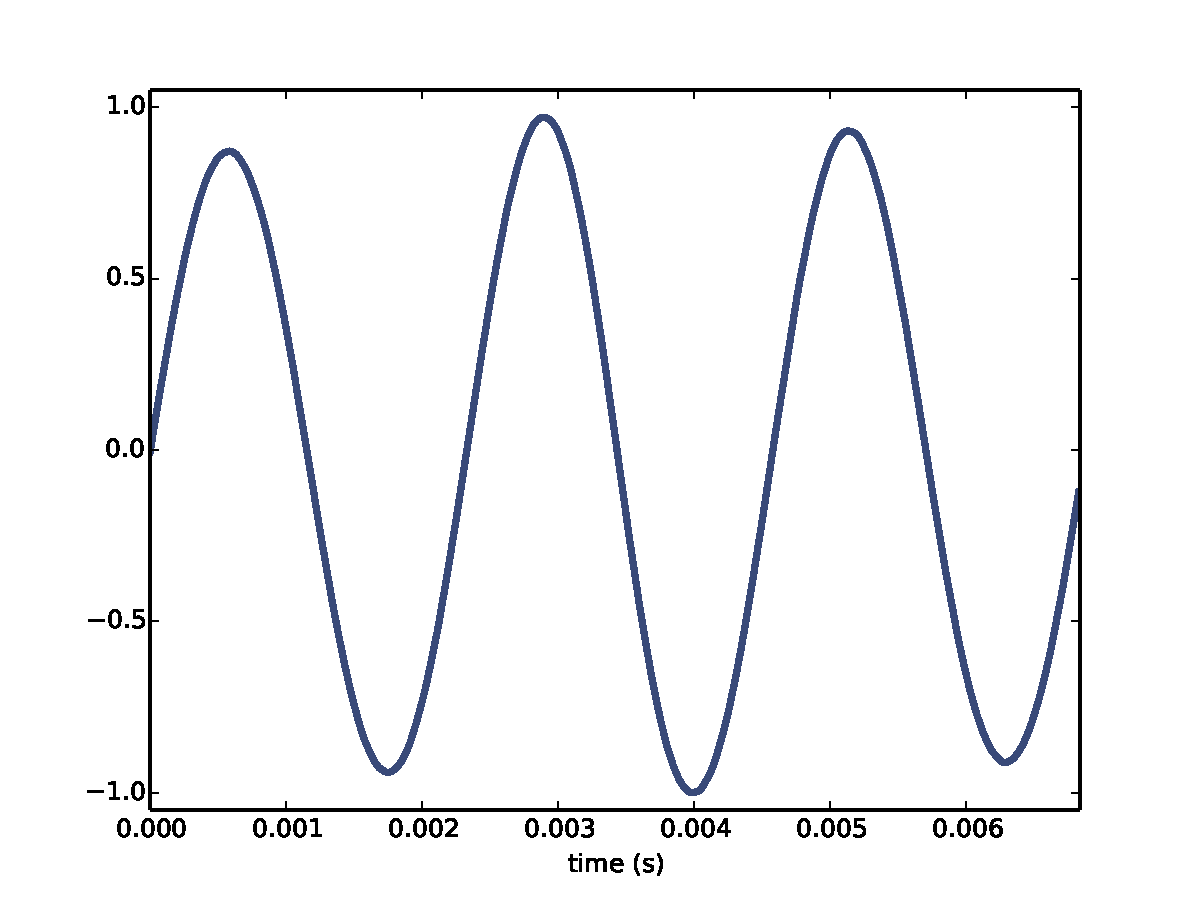
\includegraphics[height=2.5in]{figs/tuning1.pdf}}
\caption{Segment from a recording of a tuning fork.}
\label{fig.tuning1}
\end{figure}

We'll start with {\bf periodic signals}, which are signals that
repeat themselves after some period of time.  For example, if you
strike a tuning fork, it vibrates and generates sound.  If you record
that sound and plot the transduced signal, it looks like
Figure~\ref{fig.tuning1}.\footnote{I got this recording from
  \url{http://www.freesound.org/people/zippi1/sounds/18871/}.}

This signal is similar to a sinusoid, which means it has the same shape as
the trigonometric sine function. 

You can see that this signal is periodic.  I chose the duration
to show three full periods, also known as {\bf cycles}.
The duration of each cycle is about 2.3 ms.

The {\bf frequency} of a signal is the number of cycles
per second, which is the inverse of the period.
The units of frequency are cycles per second, or {\bf Hertz},
abbreviated ``Hz''.

The frequency of this signal is about 439 Hz, slightly lower than 440
Hz, which is the standard tuning pitch for orchestral music.  The
musical name of this note is A, or more specifically, A4.  If you are
not familiar with ``scientific pitch notation'', the numerical suffix
indicates which octave the note is in.  A4 is the A above middle C.
A5 is one octave higher.  See
\url{http://en.wikipedia.org/wiki/Scientific_pitch_notation}.

\begin{figure}
% sounds.py
\centerline{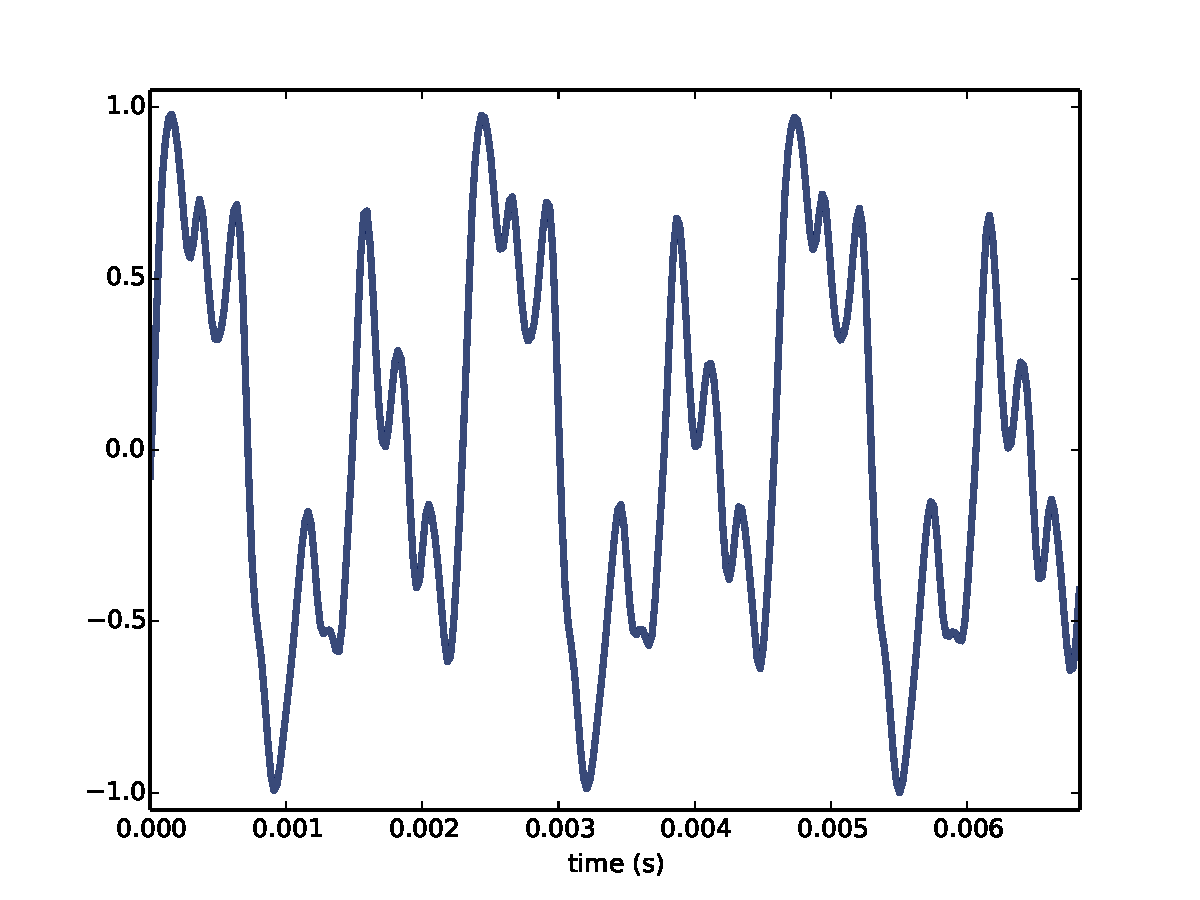
\includegraphics[height=2.5in]{figs/violin1.pdf}}
\caption{Segment from a recording of a violin.}
\label{fig.violin1}
\end{figure}

A tuning fork generates a sinusoid because the vibration of the tines
is a form of simple harmonic motion.  Most musical instruments
produce periodic signals, but the shape of these signals is not
sinusoidal.  For example, Figure~\ref{fig.violin1} shows a segment
from a recording of a violin playing
Boccherini's String Quintet No. 5 in E, 3rd
movement.\footnote{The recording is from
  \url{http://www.freesound.org/people/jcveliz/sounds/92002/}.
I identified the piece using \url{http://www.musipedia.org}.}

% Parson's code: DUUDDUURDR

Again we can see that the signal is periodic, but the shape of the
signal is more complex.  The shape of a periodic signal is called
the {\bf waveform}.  Most musical instruments produce waveforms more
complex than a sinusoid.  The shape of the waveform determines the
musical {\bf timbre}, which is our perception of the quality of the
sound.  People usually perceive complex waveforms as rich, warm and
more interesting than sinusoids.


\section{Spectral decomposition}

\begin{figure}
% sounds.py
\centerline{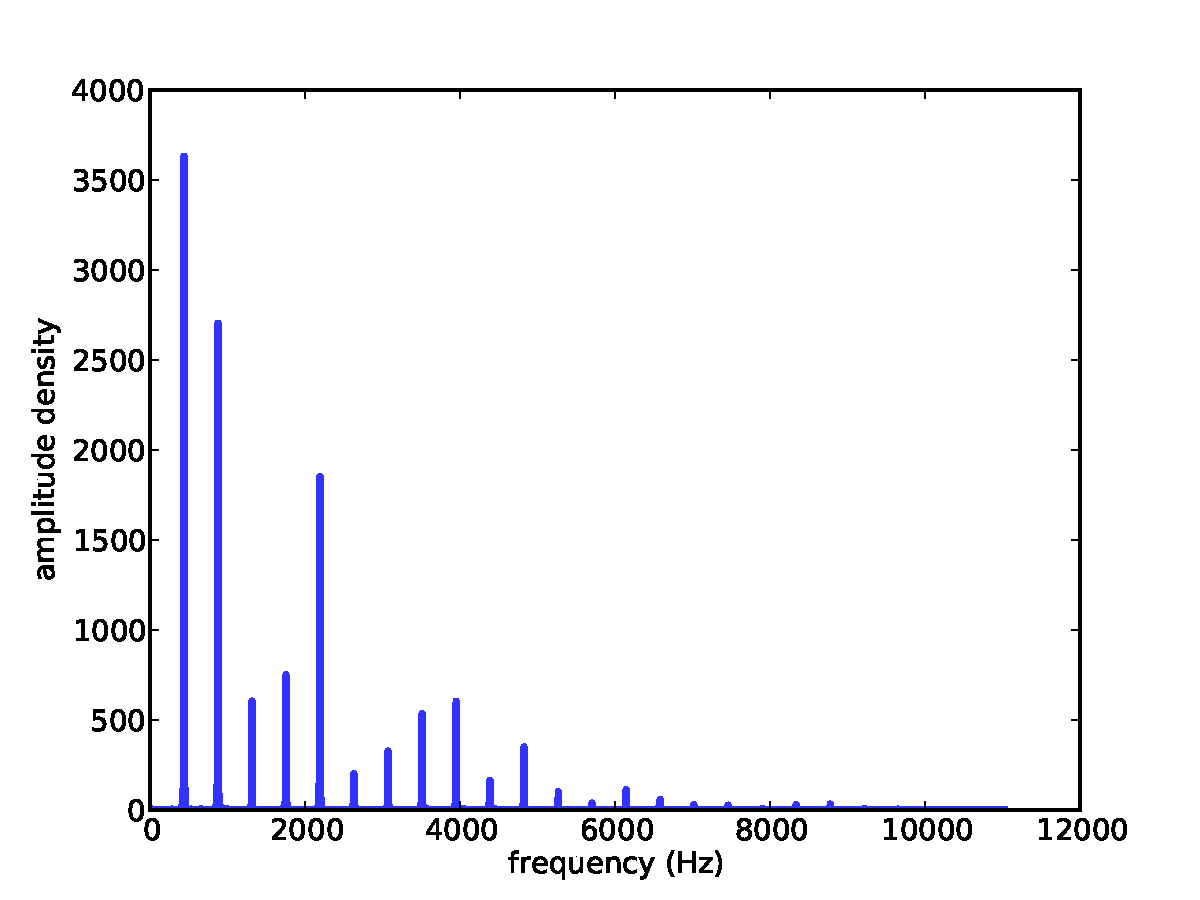
\includegraphics[height=2.5in]{figs/violin2.pdf}}
\caption{Spectrum of a segment from the violin recording.}
\label{fig.violin2}
\end{figure}

The most important topic in this book is {\bf spectral decomposition},
which is the idea that a complex signal can be expressed as the sum of
simpler signals with different frequencies.

And the most important algorithm in this book is the {\bf discrete
  Fourier transform}, or {\bf DFT}, which takes a signal (a quantity
varying in time) and produces its {\bf spectrum}, which is the set of
sinusoids that add up to produce the signal.

For example, Figure~\ref{fig.violin2} shows the spectrum of the violin
recording in Figure~\ref{fig.violin1}.  The x-axis is the range of
frequencies that make up the signal.  The y-axis shows the strength of
each frequency component.

The lowest frequency component is called the {\bf fundamental
  frequency}.  The fundamental frequency of this signal is near 440 Hz
(actually a little lower, or ``flat'').

In this signal the fundamental frequency has the largest amplitude,
so it is also the {\bf dominant frequency}.
Normally the perceived pitch of a sound is determined by the
fundamental frequency, even if it is not dominant. 

The other spikes in the spectrum are at frequencies 880, 1320, 1760, and
2200, which are integer multiples of the fundamental.
These components are called {\bf harmonics} because they are
musically harmonious with the fundamental:

\begin{itemize}

\item 880 is the frequency of
A5, one octave higher than the fundamental.  

\item 1320 is approximately E6, which is a major fifth\footnote{If you
  are not familiar with musical intervals like "major fifth'', see
  \url{https://en.wikipedia.org/wiki/Interval_(music)}.} above A5.

\item 1760 is A6, two octaves above the fundamental. 

\item 2200 is approximately C$\sharp$7, which is a major third
above A6.

\end{itemize}

These harmonics make up the notes of an A major
chord, although not all in the same octave.  Some of them are only
approximate because the notes that make up Western music have been
adjusted for {\bf equal temperament} (see
 \url{http://en.wikipedia.org/wiki/Equal_temperament}).

Given the harmonics and their amplitudes, you can reconstruct the
signal by adding up sinusoids.  
Next we'll see how.


\section{Signals}

I wrote a Python module called {\tt thinkdsp} that contains
classes and functions for working with signals and spectrums.
\footnote{In Latin the plural of ``spectrum'' is ``spectra'', but 
since I am not writing in Latin, I
generally use standard English plurals.}  You can download
it from \url{http://think-dsp.com/thinkdsp.py}.

To represent signals, {\tt thinkdsp} provides a class called
{\tt Signal}, which is the parent class for several signal types,
including {\tt Sinusoid}, which represents both sine and cosine
signals.

{\tt thinkdsp} provides functions to create sine and cosine signals:

\begin{verbatim}
    cos_sig = thinkdsp.CosSignal(freq=440, amp=1.0, offset=0)
    sin_sig = thinkdsp.SinSignal(freq=880, amp=0.5, offset=0)
\end{verbatim}

{\tt freq} is frequency in Hz.  {\tt amp} is amplitude in unspecified
units where 1.0 is generally the largest amplitude we can play.

{\tt offset} is a {\bf phase offset} in radians.
Phase offset determines where in the period the signal starts
(that is, when {\tt t=0}).  For example, a cosine signal with {\tt
  offset=0} starts at $\cos 0$, which is 1.  With {\tt offset=pi/2} it
starts at $\cos \pi/2$, which is 0.
A sine signal with
{\tt offset=0} also starts at 0.  In fact,
a cosine signal with {\tt offset=pi/2} is identical to a sine
signal with {\tt offset=0}.

Signals have an \verb"__add__" method, so you can use the {\tt +}
operator to add them:

\begin{verbatim}
    mix = sin_sig + cos_sig
\end{verbatim}

The result is a {\tt SumSignal}, which represents the sum of two
or more signals.

A Signal is basically a Python representation of a mathematical
function.  Most signals are defined for all values of {\tt t},
from negative infinity to infinity.

You can't do much with a Signal until you evaluate it.  In this
context, ``evaluate'' means taking a sequence of {\tt ts} and
computing the corresponding values of the signal, which I call {\tt
  ys}.  I encapsulate {\tt ts} and {\tt ys} in an object called a
Wave.

A Wave represents a signal evaluated at a sequence of points in
time.  Each point in time is called a {\bf frame} (a term borrowed
from movies and video).  The measurement itself is called a
{\bf sample}, although ``frame'' and ``sample'' are sometimes
used interchangeably.

{\tt Signal} provides \verb"make_wave", which returns a new
Wave object:

\begin{verbatim}
    wave = mix.make_wave(duration=0.5, start=0, framerate=11025)
\end{verbatim}

{\tt duration} is the length of the Wave in seconds.  {\tt start} is
the start time, also in seconds.  {\tt framerate} is the (integer)
number of frames per second, which is also the number of samples
per second.

11,025 frames per second is one of several framerates commonly used in
audio file formats, including Waveform Audio File (WAV) and mp3. 

This example evaluates the signal from {\tt t=0} to {\tt t=0.5} at
5,513 equally-spaced frames (because 5,513 is half of 11,025).
The time between frames, or {\bf timestep}, is {\tt 1/11025} seconds, or
91 $\mu$s.

{\tt Wave} provides a {\tt plot} method that uses {\tt pyplot}.
You can plot the wave like this:

\begin{verbatim}
    wave.plot()
    pyplot.show()
\end{verbatim}

{\tt pyplot} is part of {\tt matplotlib}; it is included in many
Python distributions, or you might have to install it.

\begin{figure}
% example1.py
\centerline{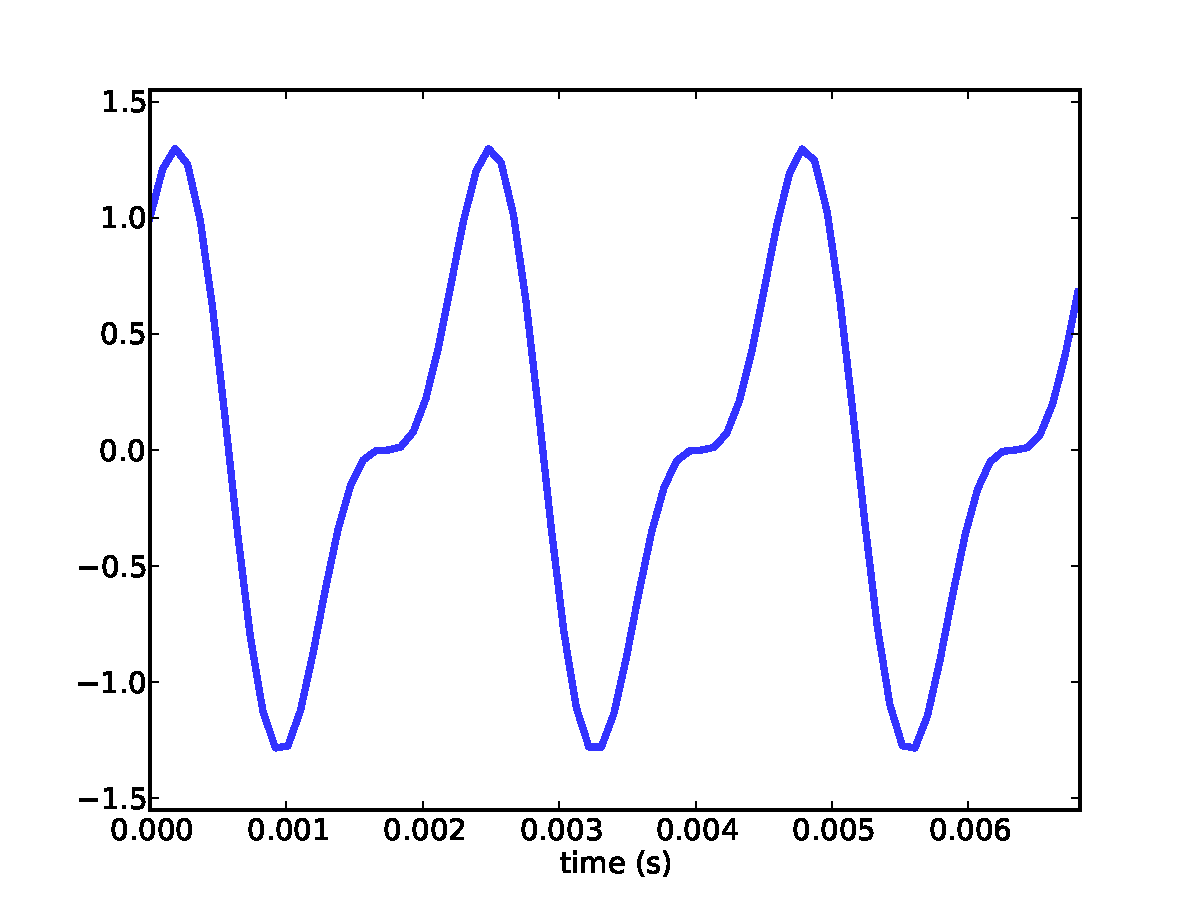
\includegraphics[height=2.5in]{figs/example1.pdf}}
\caption{Segment from a mixture of two sinusoid signals.}
\label{fig.example1}
\end{figure}

At {\tt freq=440} there are 220 periods in 0.5 seconds, so this plot
would look like a solid block of color.  To zoom in on a small number
of periods, we can use {\tt segment}, which copies a segment of a Wave
and returns a new wave:

\begin{verbatim}
    period = mix.period
    segment = wave.segment(start=0, duration=period*3)
\end{verbatim}

{\tt period} is a property of a Signal; it returns the period in second.

{\tt start} and {\tt duration} are in seconds.  This example copies
the first three periods from {\tt mix}.  If we plot {\tt segment}, it
looks like Figure~\ref{fig.example1}.  This signal contains two
frequency components, so it is more complex than the signal from the
tuning fork, but less complex than the violin.


\section{Reading and writing Waves}

{\tt thinkdsp} provides \verb"read_wave", which reads a WAV
file and returns a Wave:

\begin{verbatim}
    violin_wave = thinkdsp.read_wave('violin1.wav')
\end{verbatim}

And {\tt Wave} provides {\tt write}, which writes a WAV file:

\begin{verbatim}
    wave.write(filename='example1.wav')
\end{verbatim}

You can listen to the Wave with any media player that plays WAV
files.  On UNIX systems, I use {\tt aplay}, which is simple, robust,
and included in many Linux distributions.  For Windows you might like
MicroWav, available from
\url{http://bellsouthpwp2.net/b/o/bobad/microwav.htm}.

{\tt thinkdsp} also provides \verb"play_wave", which runs
the media player as a subprocess:

\begin{verbatim}
    thinkdsp.play_wave(filename='example1.wav', player='aplay')
\end{verbatim}

It uses {\tt aplay} by default, but you can provide another player.


\section{Spectrums}
\label{spectrums}

{\tt Wave} provides \verb"make_spectrum", which returns a
{\tt Spectrum}:

\begin{verbatim}
    spectrum = wave.make_spectrum()
\end{verbatim}

And {\tt Spectrum} provides {\tt plot}:

\begin{verbatim}
    spectrum.plot()
    thinkplot.show()
\end{verbatim}

{\tt thinkplot} is a module I wrote to provide wrappers around some of
the functions in {\tt pyplot}.  You can download it from
\url{http://think-dsp.com/thinkplot.py}.  It is also included in the
Git repository for this book (see Section~\ref{code}).

{\tt Spectrum} provides three methods that modify the spectrum:

\begin{itemize}

\item \verb"low_pass" applies a low-pass filter, which means that
  components above a given cutoff frequency are attenuated (that is,
  reduced in magnitude) by a factor.

\item \verb"high_pass" applies a high-pass filter, which means that
  it attenuates components below the cutoff.

\item \verb"band_stop" attenuates components in a the band of
frequencies between two cutoffs.

\end{itemize}

This example attenuates all frequencies above 600 by 99\%:

\begin{verbatim}
   spectrum.low_pass(cutoff=600, factor=0.01)
\end{verbatim}

Finally, you can convert a Spectrum back to a Wave:

\begin{verbatim}
    wave = spectrum.make_wave()
\end{verbatim}

At this point you know how to use many of the classes and functions in
{\tt thinkdsp}, and you are ready to do the exercises at the end of
the chapter.  In Chapter~\ref{harmonics} I explain more
about how these classes are implemented.



\section{Exercises}

Before you begin this exercises, you should download the code
for this book, following the instructions in Section~\ref{code}.

\begin{exercise}
If you have IPython, load {\tt chap01.ipynb}, read through it,
and run the examples.

Go to \url{http://freesound.org} and download a sound sample that
include music, speech, or other sounds that have a well-defined pitch.
Select a segment with duration 0.5 to 2 seconds where the pitch is
constant.  Compute and plot the spectrum of the segment you selected.
What connection can you make between the timbre of the sound and the
harmonic structure you see in the spectrum?

Use \verb"high_pass", \verb"low_pass", and \verb"band_stop" to
filter out some of the harmonics.  Then convert the spectrum back
to a wave and listen to it.  How does the sound relate to the
changes you made in the spectrum?
\end{exercise}


\begin{exercise}
Synthesize a wave by creating a spectrum with arbitrary harmonics,
inverting it, and listening.  What happens as you add frequency
components that are not multiples of the fundamental?
\end{exercise}


\begin{exercise}
This exercise asks you to write a function that simulates the
effect of sound transmission underwater.
This is a more open-ended exercise for ambitious readers.
It uses decibels, which you can read about at
\url{http://en.wikipedia.org/wiki/Decibel}.

First some background information: when sound travels through water,
high frequency components are absorbed more than low frequency
components.  In pure water, the absorption rate, expressed in decibels
per kilometer (dB/km), is proportional to frequency squared.

For example, if the absorption rate for frequency $f$ is 1 dB/km,
we expect the absorption rate for $2f$ to be 4 dB/km.  In other words,
doubling the frequency quadruples the absorption rate.

Over a distance of 10 kilometers, the $f$ component would be attenuated
by 10 dB, which corresponds to a factor of 10 in power, or a factor
of 3.162 in amplitude.  

Over the same distance, the $2f$ component would be attenuated by
40 dB, or a factor or 100 in amplitude.

Write a function that takes a Wave and returns a new Wave that contains
the same frequency components as the original, but where each
component is attenuated according to the absorption rate of water.
Apply this function to the violin recording to see what a violin
would sound like under water.

For more about the physics of sound transmission in water, see
``Underlying physics and mechanisms for the absorption of sound in
seawater'' at
\url{http://resource.npl.co.uk/acoustics/techguides/seaabsorption/physics.html}

\end{exercise}




\chapter{Harmonics}
\label{harmonics}

The code for this chapter is in {\tt aliasing.py}, which is in the
repository for this book (see Section~\ref{code}).


\section{Implementing Signals and Spectrums}

If you have done the exercises, you know how to use the classes and
methods in {\tt thinkdsp}.  Now let's see how they work.

We'll start with {\tt CosSignal} and {SinSignal}:

\begin{verbatim}
def CosSignal(freq=440, amp=1.0, offset=0):
    return Sinusoid(freq, amp, offset, func=numpy.cos)

def SinSignal(freq=440, amp=1.0, offset=0):
    return Sinusoid(freq, amp, offset, func=numpy.sin)
\end{verbatim}

These functions are just wrappers for {\tt Sinusoid}, which
is a kind of Signal:

\begin{verbatim}
class Sinusoid(Signal):
    
    def __init__(self, freq=440, amp=1.0, offset=0, func=numpy.sin):
        Signal.__init__(self)
        self.freq = freq
        self.amp = amp
        self.offset = offset
        self.func = func
\end{verbatim}

The parameters of \verb"__init__" are:

\begin{itemize}

\item {\tt freq}: frequency in cycles per second, or Hz.

\item {\tt amp}: amplitude.  The units of amplitude are arbitrary,
usually chosen so 1.0 corresponds to the maximum input from a
microphone or maximum output to a speaker.

\item {\tt offset}: where in its period the signal starts, at $t=0$.
{\tt offset} is in units of radians, for reasons I explain below.

\item {\tt func}: a Python function used
to evaluate the signal at a particular point in time.  It is
usually either {\tt numpy.sin} or {\tt numpy.cos}, yielding a sine or
cosine signal.

\end{itemize}

Like many \verb"__init__" methods, this one just tucks the
parameters away for future use.

The parent class of {\tt Sinusoid}, {\tt Signal}, provides \verb"make_wave":

\begin{verbatim}
    def make_wave(self, duration=1, start=0, framerate=11025):
        dt = 1.0 / framerate
        ts = numpy.arange(start, duration, dt)
        ys = self.evaluate(ts)
        return Wave(ys, framerate)
\end{verbatim}

{\tt start} and {\tt duration} are the start time and duration
in seconds.  {\tt framerate} is the number of frames (samples)
per second.

{\tt dt} is the time between samples, and {\tt ts} is the sequence
of sample times.

\verb"make_wave" invokes {\tt evaluate}, which has to be provided
by a child class of {\tt Signal}, in this case {\tt Sinusoid}.

{\tt evaluate} takes the sequence of sample times and returns an array of
corresponding quantities:

\begin{verbatim}
    def evaluate(self, ts):
        phases = PI2 * self.freq * ts + self.offset
        ys = self.amp * self.func(phases)
        return ys
\end{verbatim}

{\tt PI2} is a constant set to $2 \ pi$.

{\tt ts} and {\tt ys} are NumPy arrays.  I use NumPy and SciPy
throughout the book.  If you are familiar with these libraries,
that's great, but I will also explain as we go along.

Let's unwind this function one step at time:

\begin{enumerate}

\item {\tt self.freq} is frequency in cycles per second, and each
  element of {\tt ts} a time in seconds, so their product is the
  number of cycles since the start time.

\item {\tt PI2} is a constant that stores $2 \pi$.  Multiplying by
  {\tt PI2} converts from cycles to {\bf phase}.  You can think of
  phase as ``cycles since the start time'' expressed in radians; each
  cycle is $2 \pi$ radians.

\item {\tt self.offset} is the phase, in radians, at the start time.
  It has the effect of shifting the signal left or right in time.

\item If {\tt self.func} is {\tt sin} or {\tt cos}, the result is a
  value between $-1$ and $+1$.

\item Multiplying by {\tt self.amp} yields a signal that ranges from
  {\tt -self.amp} to {\tt +self.amp}.

\end{enumerate}

In math notation, {\tt evaluate} is written like this:
%
\[ A \cos (2 \pi f t + \phi_0) \]
%
where $A$ is amplitude, $f$ is frequency, $t$ is time, and $\phi_0$
is the phase offset.  It may seem like I wrote a lot of code
to evaluate one simple function, but as we'll see, this code
provides a framework for dealing with all kinds of signals, not
just sinusoids.


\section{Computing the spectrum}

Given a Signal, we can compute a Wave.  Given a Wave, we can compute
a Spectrum.  {\tt Wave} provides \verb"make_spectrum", which returns
a new {\tt Spectrum} object.

\begin{verbatim}
    def make_spectrum(self):
        hs = numpy.fft.rfft(self.ys)
        return Spectrum(hs, self.framerate)
\end{verbatim}

\verb"make_spectrum" uses {\tt rfft}, which computes
the discrete Fourier transform using an algorithm called
{\bf Fast Fourier Transform} or FFT.

The result of {\tt rfft} is a sequence of complex numbers, {\tt hs},
which is stored in a Spectrum.

There are two ways to think about
complex numbers:

\begin{itemize}

\item A complex number is the sum of a real part and an imaginary
part, often written $x + iy$, where $i$ is the imaginary unit, $\sqrt{-1}$.
You can think of $x$ and $y$ as Cartesian coordinates.

\item A complex number is also the product of a magnitude
and a complex exponential, $A e^{i \phi}$, where $A$ is the
{\bf magnitude} and $\phi$ is the
{\bf angle} in radians, also called the ``argument.''   You
can think of $A$ and $\phi$ as polar coordinates.

\end{itemize}

Each element of {\tt hs} corresponds to a frequency component.  The
magnitude of each element is proportional to the amplitude of the
corresponding component.  The angle of each element is the phase
offset.

NumPy provides {\tt absolute}, which computes the magnitude of a
complex number, also called the ``absolute value,'' and {\tt angle},
which computes the angle.

Here is the definition of {\tt Spectrum}:

\begin{verbatim}
class Spectrum(object):

    def __init__(self, hs, framerate):
        self.hs = hs
        self.framerate = framerate

        n = len(hs)
        f_max = framerate / 2.0
        self.fs = numpy.linspace(0, f_max, n)

        self.amps = numpy.absolute(self.hs)
\end{verbatim}

Again, {\tt hs} is the result of the FFT and {\tt framerate}
is the number of frames per second.

The elements of {\tt hs} correspond to a sequence of frequencies, {\tt
  fs}, equally spaced from 0 to the maximum frequency, \verb"f_max".
The maximum frequency is {\tt framerate/2}, for reasons we'll see
soon.

Finally, {\tt amps} contains the magnitude of {\tt hs}, which
is proportional to the amplitude of the components.

{\tt Spectrum} also provides {\tt plot}, which plots the magnitude for
each frequency:

\begin{verbatim}
    def plot(self, low=0, high=None):
        thinkplot.plot(self.fs[low:high], self.amps[low:high])
\end{verbatim}

{\tt low} and {\tt high} specify the slice of the Spectrum that
should be plotted.


\section{Other waveforms}

A sinusoid contains only one frequency component, so its DFT
has only one peak.  More complex waveforms, like the
violin recording, yield DFTs with many peaks.  In this section we
investigate the relationship between waveforms and their DFTs.

\begin{figure}
% example2.py
\centerline{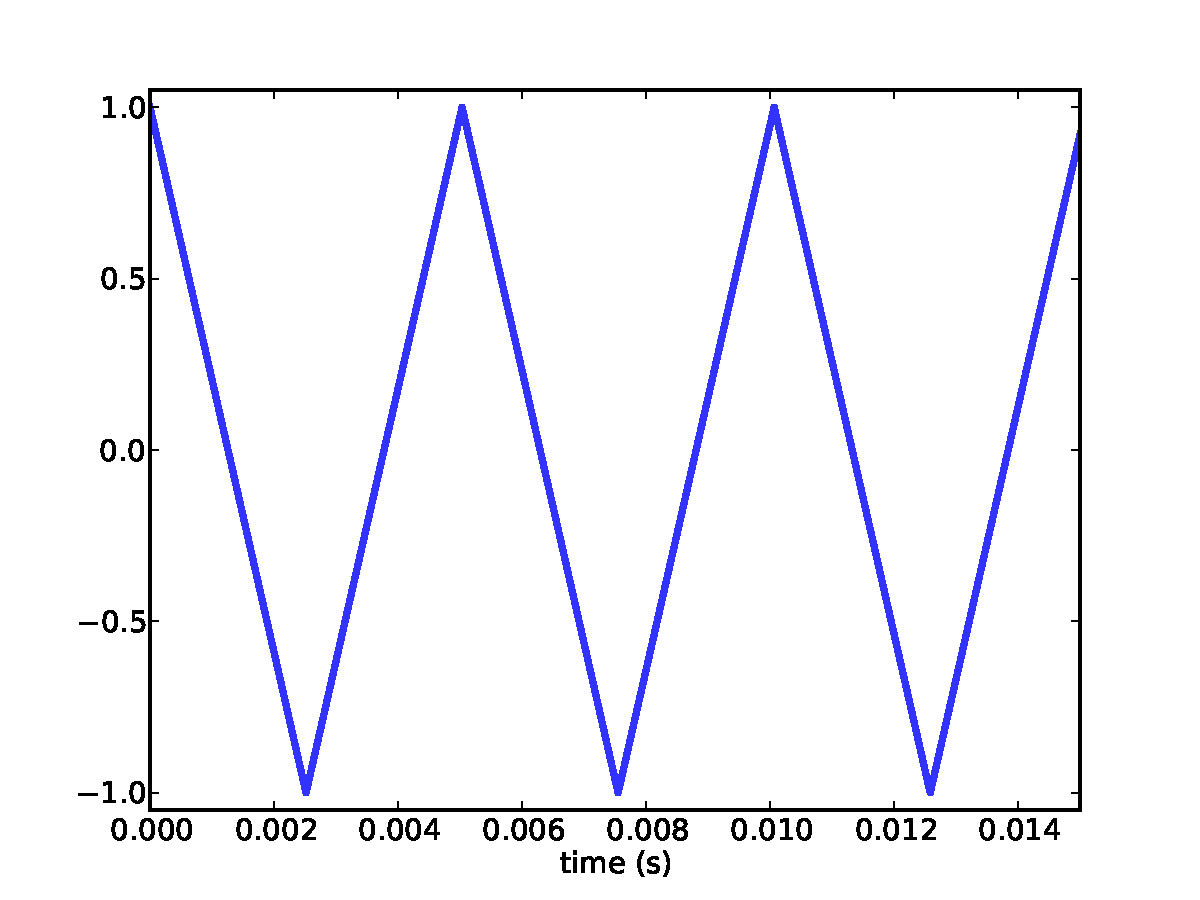
\includegraphics[height=2.5in]{figs/triangle-200-1.pdf}}
\caption{Segment of a triangle signal at 200 Hz.}
\label{fig.triangle.200.1}
\end{figure}

I'll start with a triangle waveform, which is like a straight-line
version of a sinusoid.  Figure~\ref{fig.triangle.200.1} shows a
triangle waveform with frequency 200 Hz.

To generate a triangle wave, you can use {\tt thinkdsp.TriangleSignal}:

\begin{verbatim}
class TriangleSignal(Sinusoid):
    
    def evaluate(self, ts):
        cycles = self.freq * ts + self.offset / PI2
        frac, _ = numpy.modf(cycles)
        ys = numpy.abs(frac - 0.5)
        ys = normalize(unbias(ys), self.amp)
        return ys
\end{verbatim}

{\tt TriangleSignal} inherits \verb"__init__" from {\tt Sinusoid},
so it takes the same arguments: {\tt freq}, {\tt amp}, and {\tt offset}.

The only difference is {\tt evaluate}.  As we saw before,
{\tt ts} is the sequence of sample times where we want to
evaluate the signal.

There are lots of ways to generate a triangle wave.  The details
are not important, but here's how {\tt evaluate} works:

\begin{enumerate}

\item {\tt cycles} is the number of cycles since the start time.
{\tt numpy.modf} splits the number of cycles into the fraction
part, stored in {\tt frac}, and the integer part, which is ignored.
\footnote{Using an underscore as a variable name is a convention that
means, ``I don't intend to use this value.''}

\item {\tt frac} is a sequence that ramps from 0 to 1 with the given
  frequency.  Subtracting 0.5 yields values between -0.5 and 0.5.
  Taking the absolute value yields a waveform that zig-zags between
  0.5 and 0.

\item {\tt unbias} shifts the waveform down so it is centered at 0, then
{\tt normalize} scales it to the given amplitude, {\tt amp}.

\end{enumerate}

Here's the code that generates Figure~\ref{fig.triangle.200.1}:

\begin{verbatim}
    signal = thinkdsp.TriangleSignal(200)
    duration = signal.period * 3
    segment = signal.make_wave(duration, framerate=10000)
    segment.plot()
\end{verbatim}


\section{Harmonics}

\begin{figure}
% example2.py
\centerline{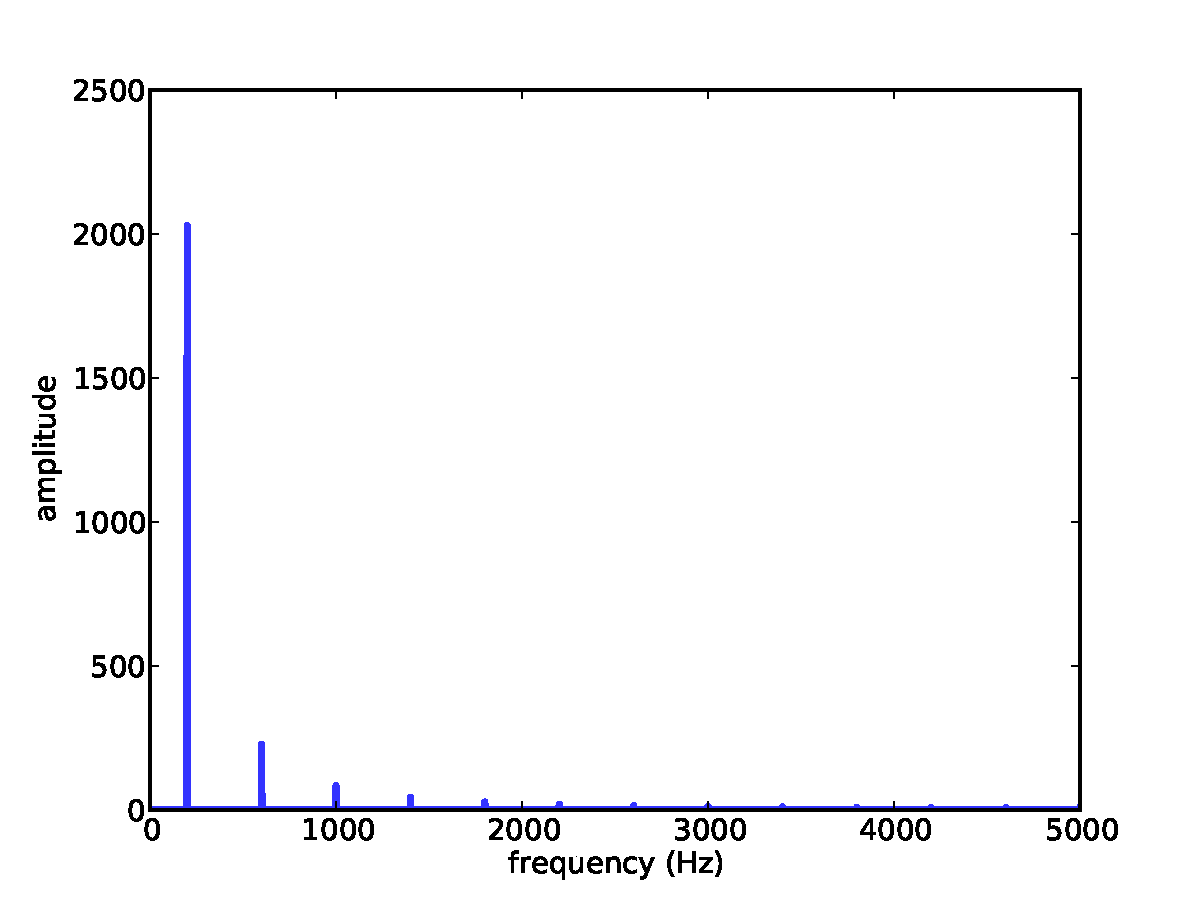
\includegraphics[height=2.5in]{figs/triangle-200-2.pdf}}
\caption{Spectrum of a triangle signal at 200 Hz.}
\label{fig.triangle.200.2}
\end{figure}

Next we can compute the spectrum of this waveform:

\begin{verbatim}
    wave = signal.make_wave(duration=0.5, framerate=10000)
    spectrum = wave.make_spectrum()
    spectrum.plot()
\end{verbatim}

Figure~\ref{fig.triangle.200.2} shows the result.  As expected, the
highest peak is at the fundamental frequency, 200 Hz, and there
are additional peaks at harmonic frequencies, which are integer
multiples of 200.

But one surprise is that there are no peaks at the even multiples:
400, 800, etc.  The harmonics of a triangle wave are all
odd multiples of the fundamental frequency, in this example
600, 1000, 1400, etc.

Another feature of this spectrum is the relationship between the
amplitude and frequency of the harmonics.  The amplitude of the
harmonics drops off in proportion to frequency squared.  For example
the frequency ratio of the first two harmonics (200 and 600 Hz) is 3,
and the amplitude ratio is approximately 9.  The frequency ratio of
the next two harmonics (600 and 1000 Hz) is 1.7, and the amplitude
ratio is approximately $1.7^2 = 2.9$.

\begin{figure}
% example2.py
\centerline{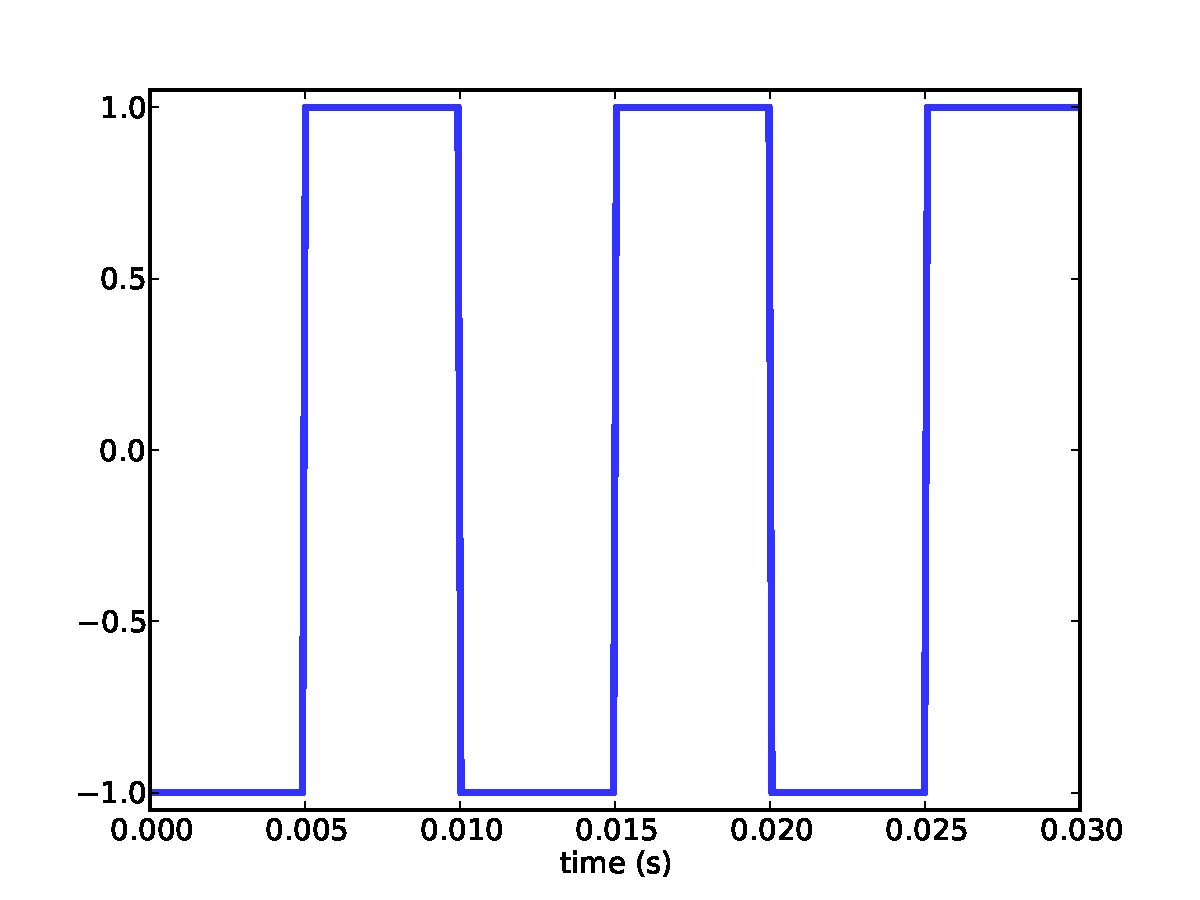
\includegraphics[height=2.5in]{figs/square-100-1.pdf}}
\caption{Segment of a square signal at 100 Hz.}
\label{fig.square.100.1}
\end{figure}

{\tt thinkdsp} also provides {\tt SquareSignal}, which represents
a square signal.  Here's the class definition:

\begin{verbatim}
class SquareSignal(Sinusoid):
    
    def evaluate(self, ts):
        cycles = self.freq * ts + self.offset / PI2
        frac, _ = numpy.modf(cycles)
        ys = self.amp * numpy.sign(unbias(frac))
        return ys
\end{verbatim}

Like {\tt TriangleSignal}, {\tt SquareSignal} inherits 
\verb"__init__" from {\tt Sinusoid}, so it takes the same
parameters.

And the {\tt evaluate} method is similar.  Again, {\tt cycles} is
the number of cycles since the start time, and {\tt frac} is the
fractional part, which ramps from 0 to 1 each period.

{\tt unbias} shifts {\tt frac} so it ramps from -0.5 to 0.5,
then {\tt numpy.sign} maps the negative values to -1 and the
positive values to 1.  Multiplying by {\tt amp} yields a square
wave that jumps between {\tt -amp} and {\tt amp}.

\begin{figure}
% example2.py
\centerline{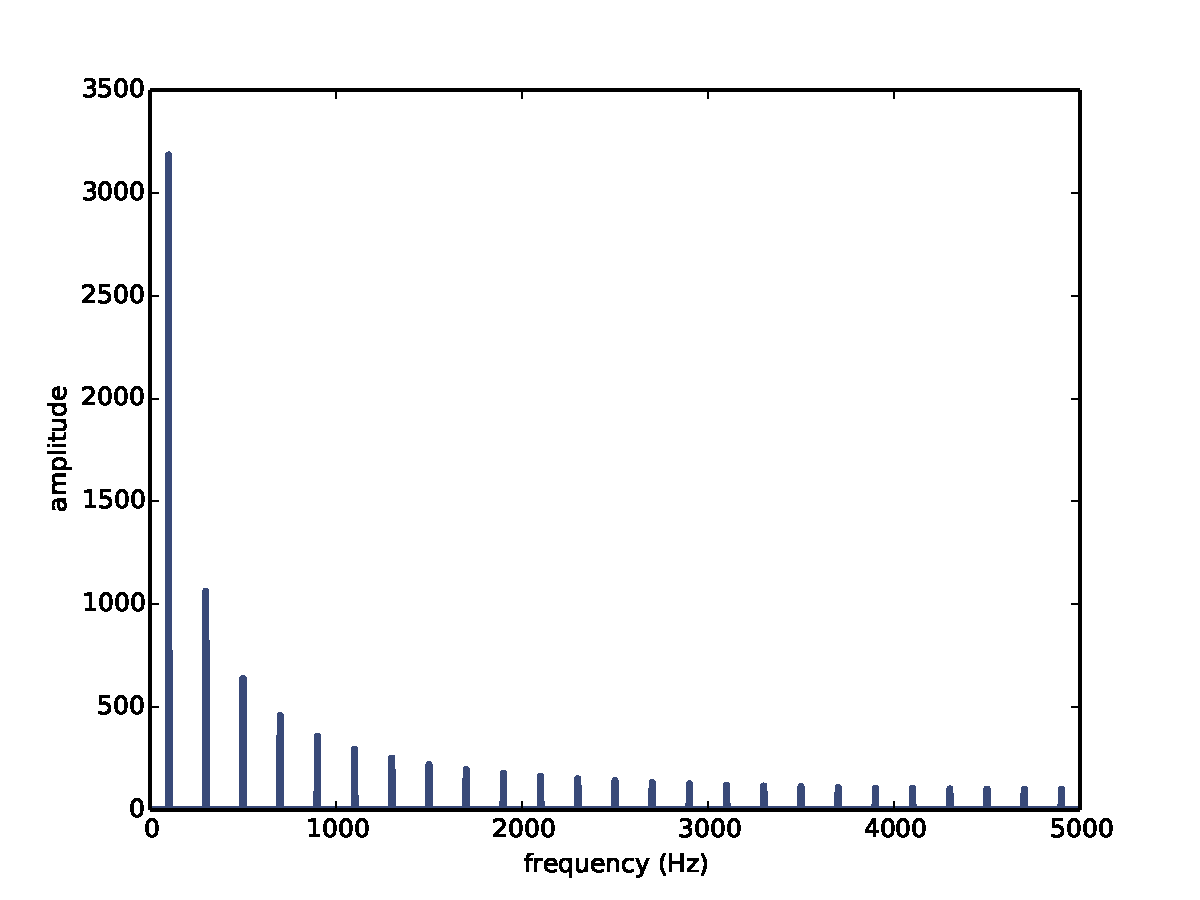
\includegraphics[height=2.5in]{figs/square-100-2.pdf}}
\caption{Spectrum of a square signal at 100 Hz.}
\label{fig.square.100.2}
\end{figure}

Figure~\ref{fig.square.100.1} shows three periods of a square
wave with frequency 100 Hz,
and Figure~\ref{fig.square.100.2} shows its spectrum.

Like a triangle wave, the square wave contains only odd harmonics,
which is why there are peaks at 300, 500, and 700 Hz, etc.
But the amplitude of the harmonics drops off more slowly.
Specifically, amplitude drops in proportion to frequency (not frequency
squared).


\section{Aliasing}
\label{aliasing}

\begin{figure}
% example2.py
\centerline{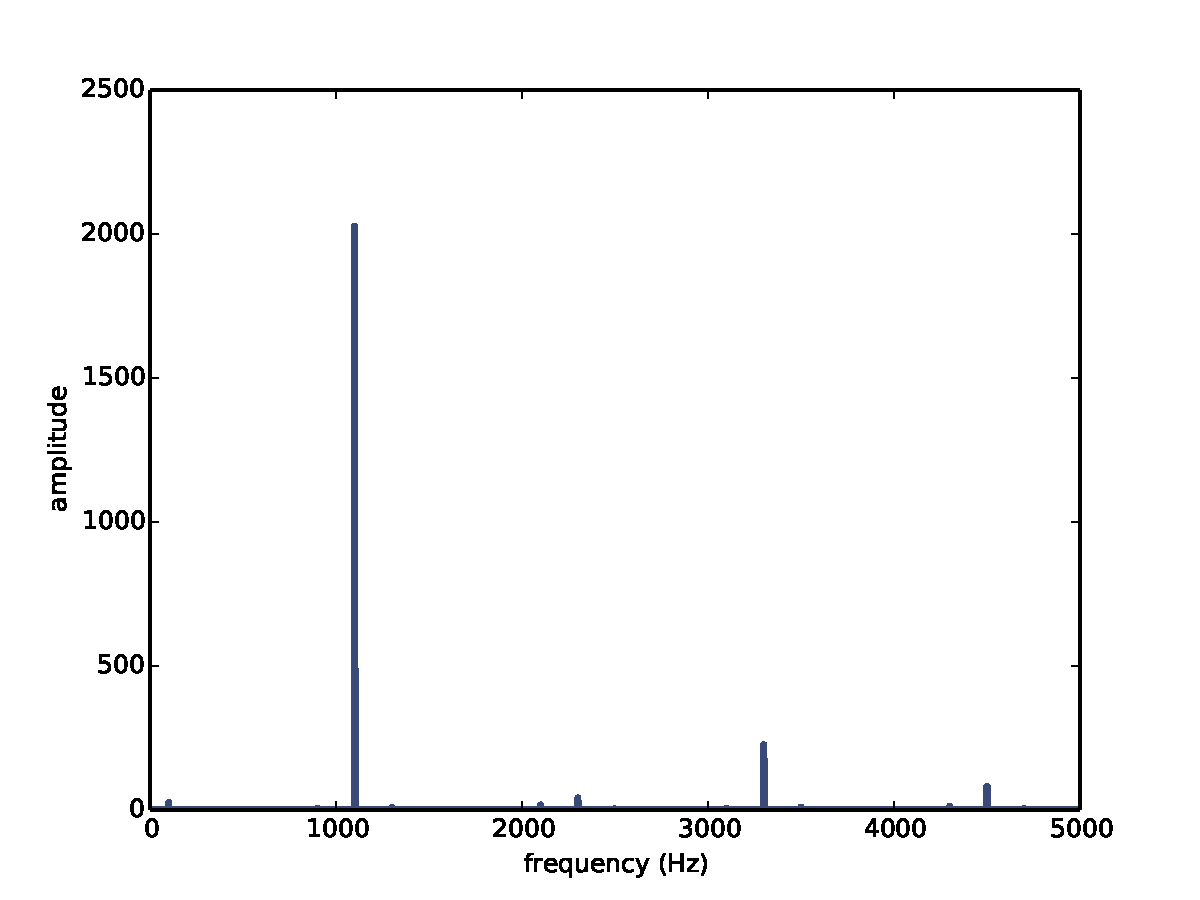
\includegraphics[height=2.5in]{figs/triangle-1100-2.pdf}}
\caption{Spectrum of a triangle signal at 1100 Hz sampled at
10,000 frames per second.}
\label{fig.triangle.1100.2}
\end{figure}

I have a confession.  I chose the examples in the previous section
carefully, to avoid showing you something confusing.  But now it's
time to get confused.

Figure~\ref{fig.triangle.1100.2} shows the spectrum of a triangle wave
at 1100 Hz, sampled at 10,000 frames per second.

As expected, there are peaks at 1100 and 3300 Hz, but the third
peak is at 4500, not 5500 Hz as expected.  There is a small fourth peak
at 2300, not 7700 Hz.  And if you look very closely, the peak that should
be at 9900 is actually at 100 Hz.  What's going on?

The problem is that when you evaluate the signal at
discrete points in time, you lose information about what happens
between samples.  For low frequency components, that's not a
problem, because you have lots of samples per period.

But if you sample a signal at 5000 Hz with 10,000 frames per second,
you only have two samples per period.  That's enough to measure the
frequency (it turns out), but it doesn't tell you much about
the shape of the signal.

If the frequency is higher, like the 5500 Hz component of the
triangle wave, things are worse: you don't even get the
frequency right.

To see why, let's generate cosine signals at 4500 and 5500 Hz,
and sample them at 10,000 frames per second:

\begin{verbatim}
    framerate = 10000

    signal = thinkdsp.CosSignal(4500)
    duration = signal.period*5
    segment = signal.make_wave(duration, framerate=framerate)
    segment.plot()

    signal = thinkdsp.CosSignal(5500)
    segment = signal.make_wave(duration, framerate=framerate)
    segment.plot()
\end{verbatim}

\begin{figure}
% example2.py
\centerline{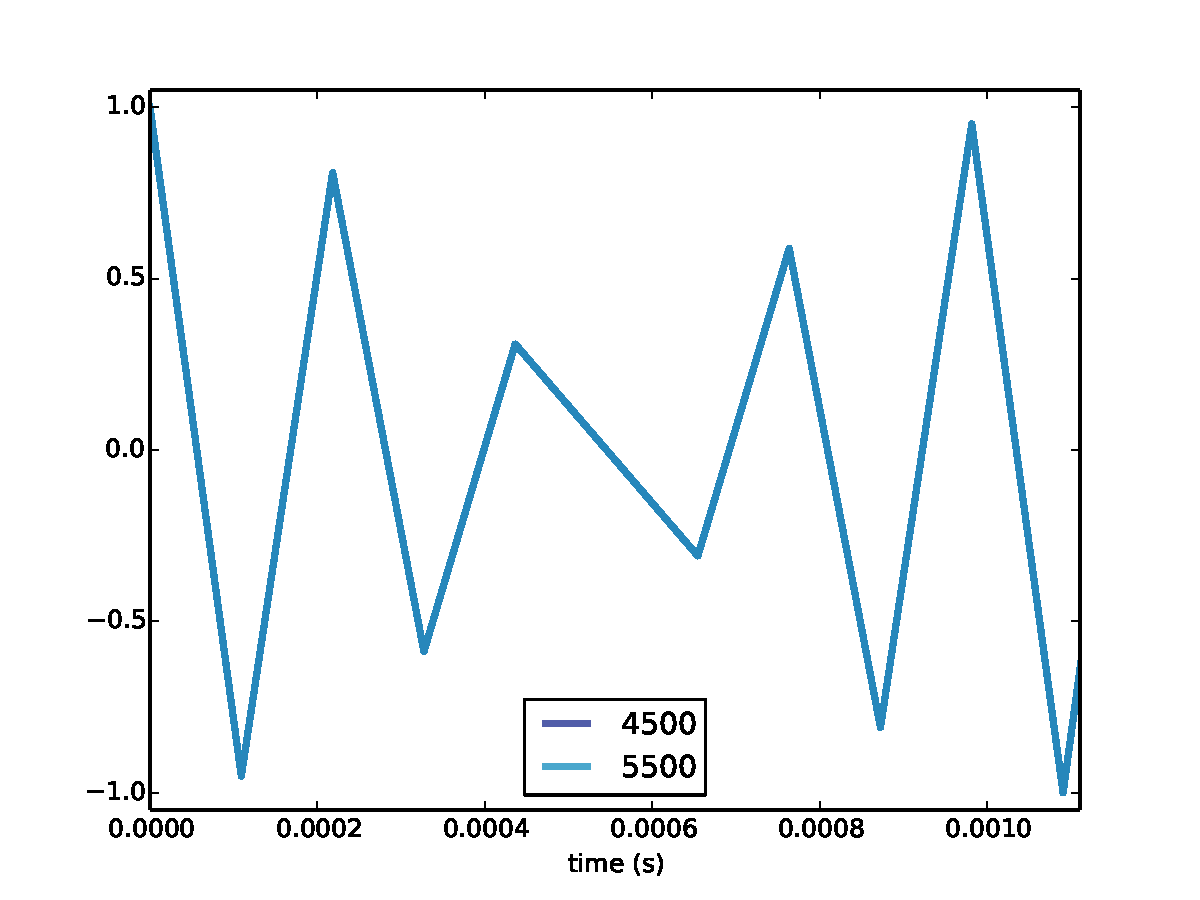
\includegraphics[height=2.5in]{figs/aliasing-3.pdf}}
\caption{Cosine signals at 4500 and 5500 Hz, sampled at 10,000 frames
per second.}
\label{fig.aliasing-3}
\end{figure}

Figure~\ref{fig.aliasing-3} shows the result.  The
sampled waveform doesn't look very much like a sinusoid, but the
bigger problem is that the two waveforms are exactly the same!

When we sample a 5500 Hz signal at 10,000 frames per second, the
result is indistinguishable from a 4500 Hz signal.

For the same reason, a 7700 Hz signal is indistinguishable
from 2300 Hz, and a 9900 Hz is indistinguishable from 100 Hz.

This effect is called {\bf aliasing} because when the high frequency
signal is sampled, it disguises itself as a low frequency signal.

In this example, the highest frequency we can measure is 5000 Hz,
which is half the sampling rate.  Frequencies above 5000 Hz are folded
back below 5000 Hz, which is why this threshold is sometimes called
the ``folding frequency,'' but more often it is called the {\bf
  Nyquist frequency}.  See
\url{http://en.wikipedia.org/wiki/Nyquist_frequency}.

The folding pattern continues if the aliased frequency goes below
zero.  For example, the 5th harmonic of the 1100 Hz triangle wave is
at 12,100 Hz.  Folded at 5000 Hz, it would appear at -2100 Hz, but it
gets folded again at 0 Hz, back to 2100 Hz.  In fact, you can see a
small peak at 2100 Hz in Figure~\ref{fig.square.100.2}, and the next
one at 4300 Hz.


\section{Exercises}

\begin{exercise}
If you use IPython, load {\tt chap02.ipynb} and try out the examples.
You can also view the notebook at \url{http://tinyurl.com/thinkdsp02}.
\end{exercise}

\begin{exercise}
A sawtooth signal has a waveform that ramps up linearly from -1 to 1,
then drops to -1 and repeats. See
\url{http://en.wikipedia.org/wiki/Sawtooth_wave}

Write a class called
{\tt SawtoothSignal} that extends {\tt Signal} and provides
{\tt evaluate} to evaluate a sawtooth signal.

Compute the spectrum of a sawtooth wave.  How does the harmonic
structure compare to triangle and square waves?
\end{exercise}

\begin{exercise}
Sample an 1100 Hz triangle at 10000 frames per second and listen to it.
Can you hear the aliased harmonic?  It might help if you play a sequence of
notes with increasing pitch.
\end{exercise}

\begin{exercise}
Compute the spectrum of an 1100 Hz square wave sampled at 10 kHz, and
compare it to the spectrum of a triangle wave in
Figure~\ref{fig.triangle.1100.2}
\end{exercise}

\begin{exercise}
The triangle and square waves have odd harmonics only; the sawtooth
wave has both even and odd harmonics.  The harmonics of the
square and sawtooth waves drop off in proportion to $1/f$; the
harmonics of the triangle wave drop off like $1/f^2$.  Can you
find a waveform that has even and odd harmonics that drop off
like $1/f$?
\end{exercise}



\chapter{Non-periodic signals}

The code for this chapter is in {\tt chirp.py}, which is in the
repository for this book (see Section~\ref{code}).


\section{Chirp}

The signals we have worked with so far are periodic, which means
that they repeat forever.  It also means that their spectrums do
not vary in time.  In this chapter, we consider non-periodic signals,
which include signals whose frequency components change over time.
In other words, pretty much all sound signals.

We'll start with a {\bf chirp}, which is a signal with variable
frequency.  Here is a class that represents a chirp:

\begin{verbatim}
class Chirp(Signal):
    
    def __init__(self, start=440, end=880, amp=1.0):
        self.start = start
        self.end = end
        self.amp = amp
\end{verbatim}

{\tt start} and {\tt end} are the frequencies, in Hz, at the start
and end of the chirp.  {\tt amp} is amplitude.

In a linear chirp, the frequency increases linearly from {\tt start}
to {\tt end}.  Here is the function that evaluates the signal:

\begin{verbatim}
    def evaluate(self, ts):
        freqs = numpy.linspace(self.start, self.end, len(ts)-1)
        return self._evaluate(ts, freqs)
\end{verbatim}

{\tt ts} is the sequence of points in time where the signal should
be evaluated.  If the length of {\tt ts} is $n$, you can think of
it as a sequence of $n-1$ intervals of time.  To compute the frequency
during each interval, we use {\tt numpy.linspace}.

\verb"_evaluate" is a private method\footnote{Beginning a method name
  with an underscore makes it ``private,'' indicating that it is not
  part of the API that should be used outside the class definition.}
that does the rest of the math:

\begin{verbatim}
    def _evaluate(self, ts, freqs):
        dts = numpy.diff(ts)
        dphis = PI2 * freqs * dts
        phases = numpy.cumsum(dphis)
        ys = self.amp * numpy.cos(phases)
        return ys
\end{verbatim}

{\tt numpy.diff} computes the difference between adjacent elements
of {\tt ts}, returning the length of each interval in seconds.  In
the usual case where the elements of {\tt ts} are equally spaced,
the {\tt dts} are all the same.

The next step is to figure out how much the phase changes during
each interval.  Since we know the frequency and duration of each
interval, the {\em change} in phase during each interval is
{\tt dphis = PI2 * freqs * dts}.  In math notation:
%
\[ \Delta \phi = 2 \pi f(t) \Delta t \]
%
{\tt numpy.cumsum} computes the cumulative sum, which you can think
of as a simple kind of integration.  The result is
a NumPy array where the {\tt i}th element contains the sum of
the first {\tt i} terms from {\tt dphis}; that is, the total
phase at the end of the {\tt i}th interval.  Finally, {\tt numpy.cos}
maps from phase to amplitude.

Here's the code that creates and plays a chirp from 220 to 880 Hz, which
is two octaves from A3 to A5:

\begin{verbatim}
    signal = thinkdsp.Chirp(start=220, end=880)
    wave1 = signal.make_wave(duration=2)

    filename = 'chirp.wav'
    wave1.write(filename)
    thinkdsp.play_wave(filename)
\end{verbatim}

You can run this code in {\tt chap03.ipynb} or view the notebook
at \url{http://tinyurl.com/thinkdsp03}.


\section{Exponential chirp}

When you listen to this chirp, you might notice that the pitch
rises quickly at first and then slows down.
The chirp spans two octaves, but it only takes 2/3 s to span
the first octave, and twice as long to span the second.  

The reason is that our perception of pitch depends on the logarithm of
frequency.  As a result, the {\bf interval} we hear between two notes
depends on the {\em ratio} of their frequencies, not the difference.
``Interval'' is the musical term for the perceived difference between
two pitches.

For example, an octave is an interval where the ratio of two
pitches is 2.  So the interval from 220 to 440 is one octave
and the interval from 440 to 880 is also one octave.  The difference
in frequency is bigger, but the ratio is the same.

As a result, if frequency increases linearly, as in a linear
chirp, the perceived pitch increases logarithmically.

If you want the perceived pitch to increase linearly, the frequency
has to increase exponentially.  A signal with that shape is called
an {\bf exponential chirp}.

Here's the code that makes one:

\begin{verbatim}
class ExpoChirp(Chirp):
    
    def evaluate(self, ts):
        start, end = math.log10(self.start), math.log10(self.end)
        freqs = numpy.logspace(start, end, len(ts)-1)
        return self._evaluate(ts, freqs)
\end{verbatim}

Instead of {\tt numpy.linspace}, this version of evaluate uses
{\tt numpy.logspace}, which creates a series of frequencies
whose logarithms are equally spaced, which means that they increase
exponentially.

That's it; everything else is the same as Chirp.  Here's the code
that makes one:

\begin{verbatim}
    signal = thinkdsp.ExpoChirp(start=220, end=880)
    wave1 = signal.make_wave(duration=2)

    filename = 'expo_chirp.wav'
    wave1.write(filename)
    thinkdsp.play_wave(filename)
\end{verbatim}

Run this code and listen.  If you have a musical ear, this might
sound more like music than the linear chirp.


\section{Leakage}

\begin{figure}
% chirp.py
\centerline{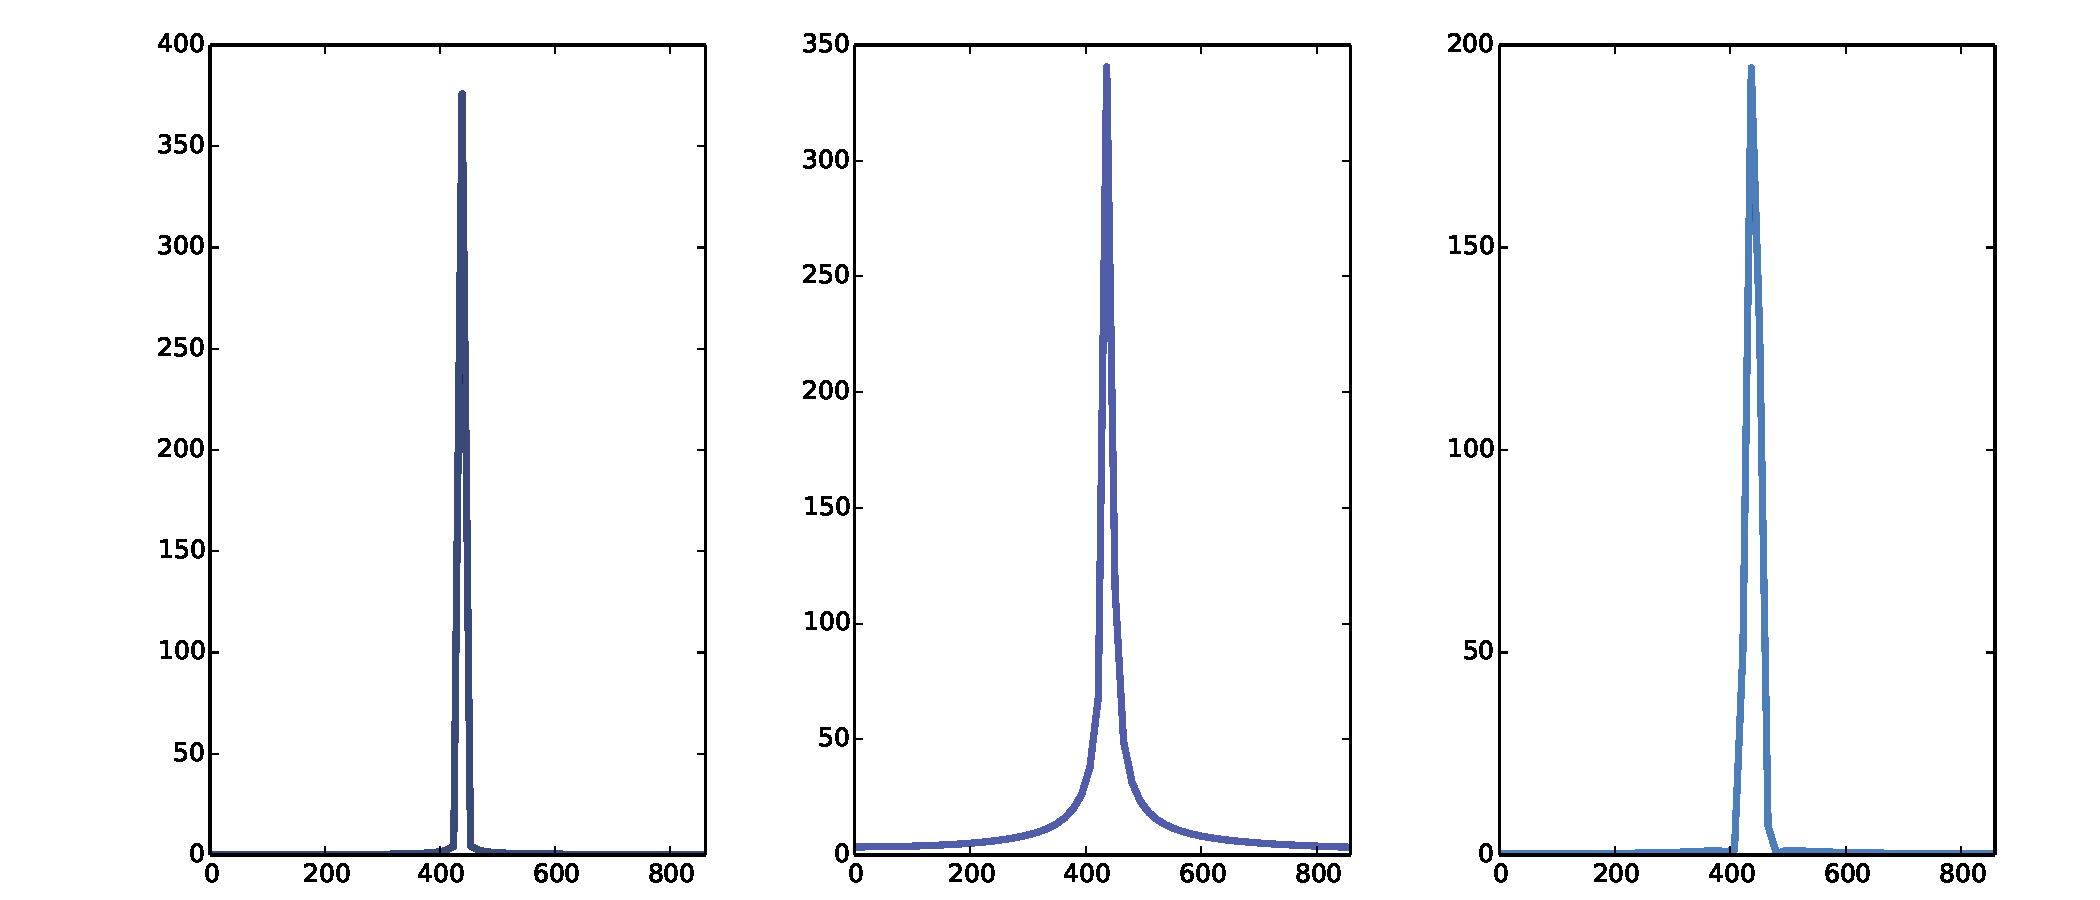
\includegraphics[height=2.5in]{figs/windowing1.pdf}}
\caption{Spectrum of (a) a periodic segment of a sinusoid, (b)
a non-periodic segment, (c) a tapered non-periodic segment.}
\label{fig.windowing1}
\end{figure}

In previous chapters, we used the Fast Fourier Transform (FFT) to
compute the spectrum of a wave.  When we discuss how FFT works in
Chapter~\ref{dft}, we will learn that it is based on the assumption
that the signal is periodic.  In theory, we should not use FFT on
non-periodic signals.  In practice it happens all the time, but there
are a few things you have to be careful about.

One common problem is dealing with discontinuities at the beginning
and end of a segment.  Because FFT assumes that the signal is periodic,
it implicitly connects the end of the segment back to the beginning
to make a loop.  If the end does not connect smoothly to the beginning,
the discontinuity creates additional frequency components in the
segment that are not in the signal.

As an example, let's start with a sine wave that contains only
one frequency component at 440 Hz.

\begin{verbatim}
    signal = thinkdsp.SinSignal(freq=440)
\end{verbatim}

If we select a segment that happens to be an integer multiple of
the period, the end of the segment connects smoothly with the
beginning, and FFT behaves well.

\begin{verbatim}
    duration = signal.period * 30
    wave = signal.make_wave(duration)
    spectrum = wave.make_spectrum()
\end{verbatim}

Figure~\ref{fig.windowing1}a shows the result.  As expected, there is
a single peak at 440 Hz.

But if the duration is not a multiple of the
period, bad things happen.  With {\tt duration = signal.period *
  30.25}, the signal starts at 0 and ends at 1.
Figure~\ref{fig.windowing1}b shows the spectrum of this segment.
Again, the peak is at 440 Hz, but now there are additional components
spread out from 240 to 640 Hz.  This spread is called ``spectral
leakage'', because some of the energy at the fundamental frequency
leaks into other frequencies.

In this example, leakage happens because we are using FFT on a segment
that is not periodic.


\section{Windowing}

\begin{figure}
% chirp.py
\centerline{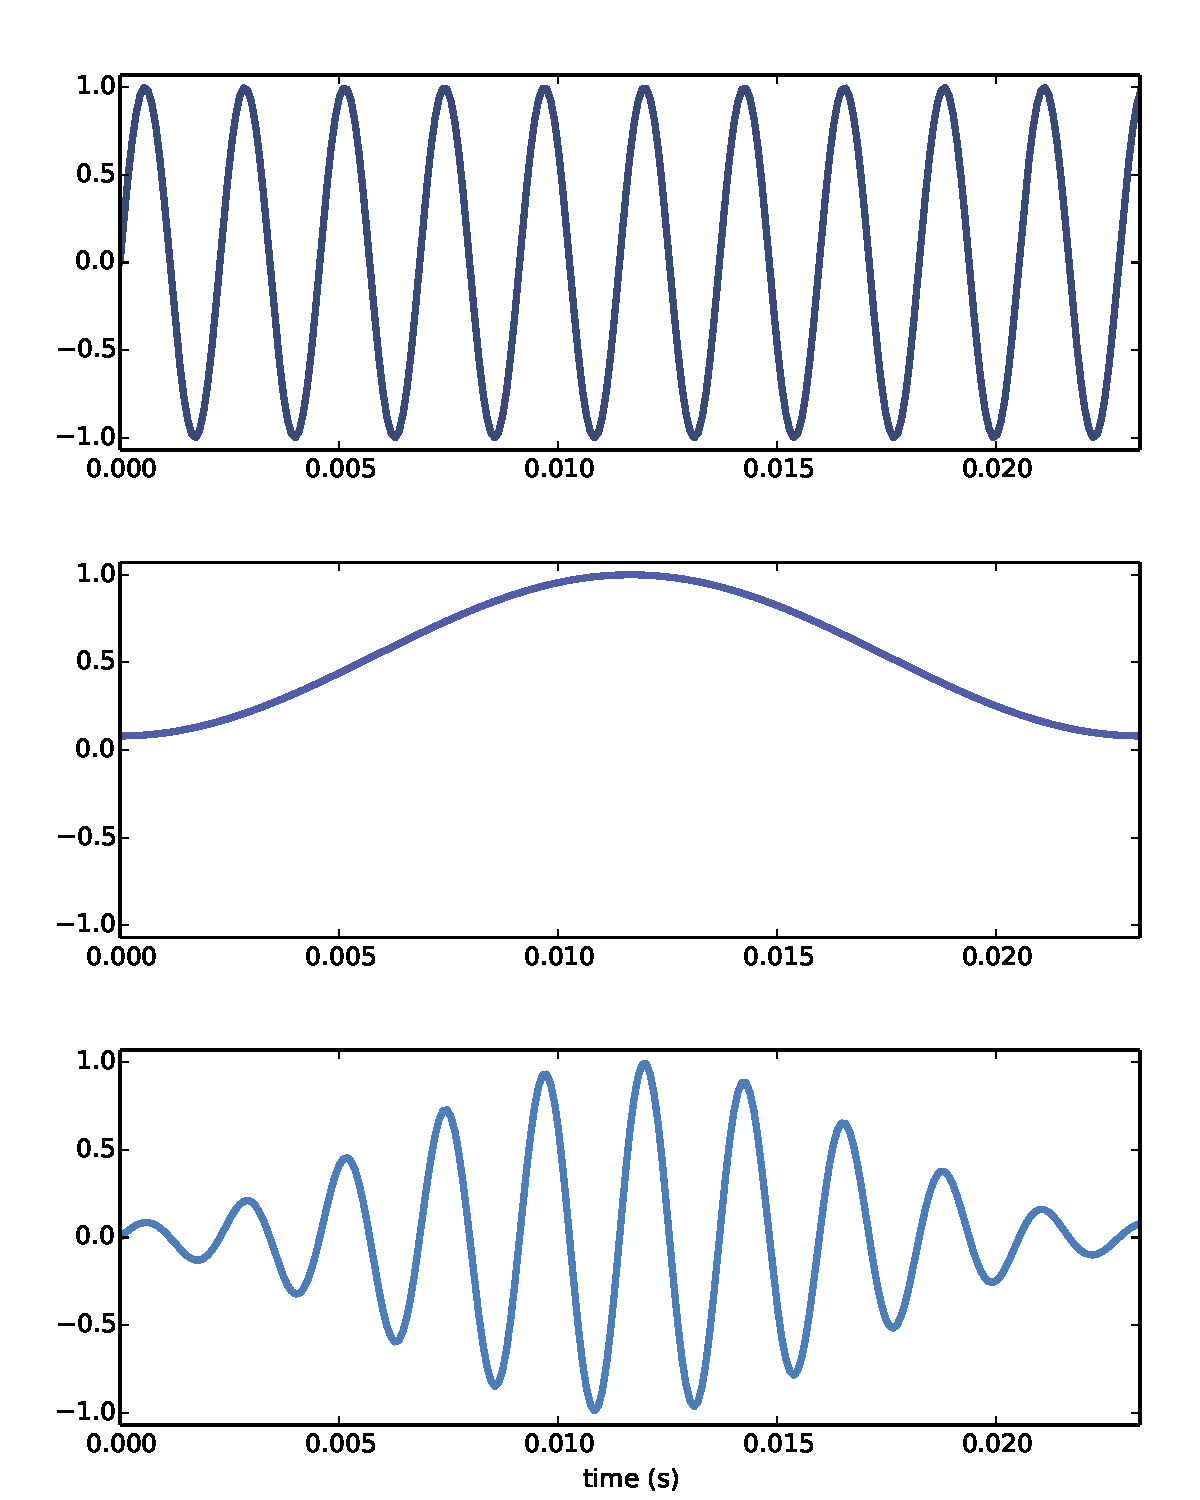
\includegraphics[height=3.5in]{figs/windowing2.pdf}}
\caption{(a) Segment of a sinusoid, (b) Hamming window, (c) product
of the segment and the window.}
\label{fig.windowing2}
\end{figure}

We can reduce leakage by smoothing out the discontinuity between
the beginning and end of the segment, and one way to do that is
{\bf windowing}.

A ``window'' is a function designed to transform a non-periodic
segment into something that can pass for periodic.
Figure~\ref{fig.windowing2}a shows a segment where the end does not
connect smoothly to the beginning.

Figure~\ref{fig.windowing2}b shows a ``Hamming window'', one of the
more common window functions.  No window function is perfect, but some
can be shown to be optimal for different applications, and Hamming
is a commonly-used, all-purpose window.

Figure~\ref{fig.windowing2}c shows the result of multiplying the
window by the original signal.  Where the window is close to 1, the
signal is unchanged.  Where the window is close to 0, the signal is
attenuated.  Because the window tapers at both ends, the end of the
segment connects smoothly to the beginning.

Figure~\ref{fig.windowing1}c shows the spectrum of the tapered signal.
Windowing has reduced leakage substantially, but not completely. 

Here's what the code looks like.  {\tt Wave} provides {\tt hamming},
which applies a Hamming window:

\begin{verbatim}
    def hamming(self):
        self.ys *= numpy.hamming(len(self.ys))
\end{verbatim}

{\tt numpy.hamming} computes the Hamming window with the given number
of elements.  NumPy provides functions to compute other window
functions, including {\tt bartlett}, {\tt blackman}, {\tt hanning},
and {\tt kaiser}.  One of the exercises at the end of this chapter
asks you to experiment with these other windows.


\section{Spectrum of a chirp}

\begin{figure}
% chirp.py
\centerline{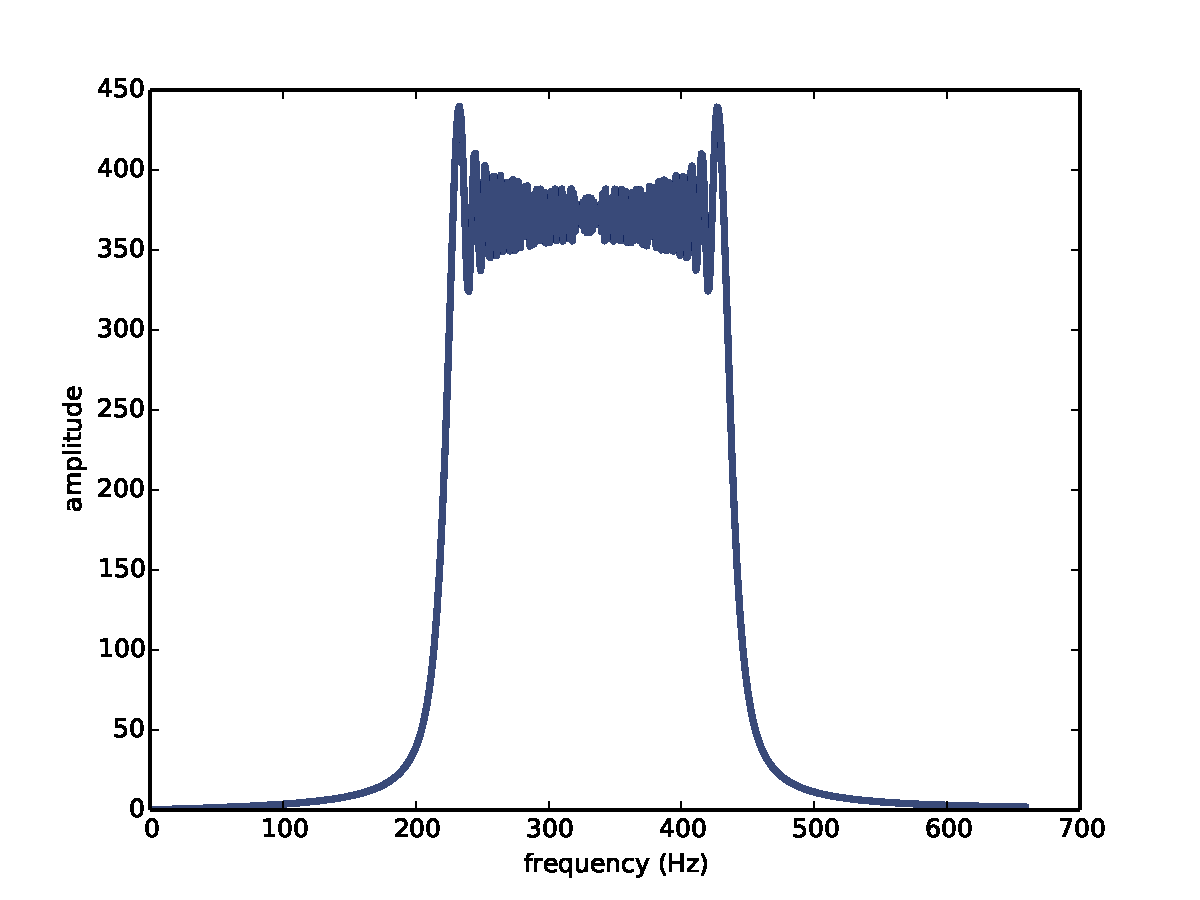
\includegraphics[height=2.5in]{figs/chirp1.pdf}}
\caption{Spectrum of a one-second one-octave chirp.}
\label{fig.chirp1}
\end{figure}

What do you think happens if you compute the spectrum of a chirp?
Here's an example that constructs a one-second one-octave chirp and
its spectrum:

\begin{verbatim}
    signal = thinkdsp.Chirp(start=220, end=440)
    wave = signal.make_wave(duration=1)
    spectrum = wave.make_spectrum()
\end{verbatim}

Figure~\ref{fig.chirp1} shows the result.  The spectrum shows
components at every frequency from 220 to 440 Hz with variations,
caused by leakage, that look a little like the Eye of Sauron
(see \url{http://en.wikipedia.org/wiki/Sauron}).

The spectrum is approximately flat between 220 and 440 Hz, which
indicates that the signal spends equal time at each frequency in this
range.  Based on that observation, you should be able to guess what
the spectrum of an exponential chirp looks like.

The spectrum gives hints about the structure of the signal,
but it loses the relationship between frequency and time.
For example, we cannot tell by looking at this spectrum whether
the frequency went up or down, or both.


\section{Spectrogram}

\begin{figure}
% chirp.py
\centerline{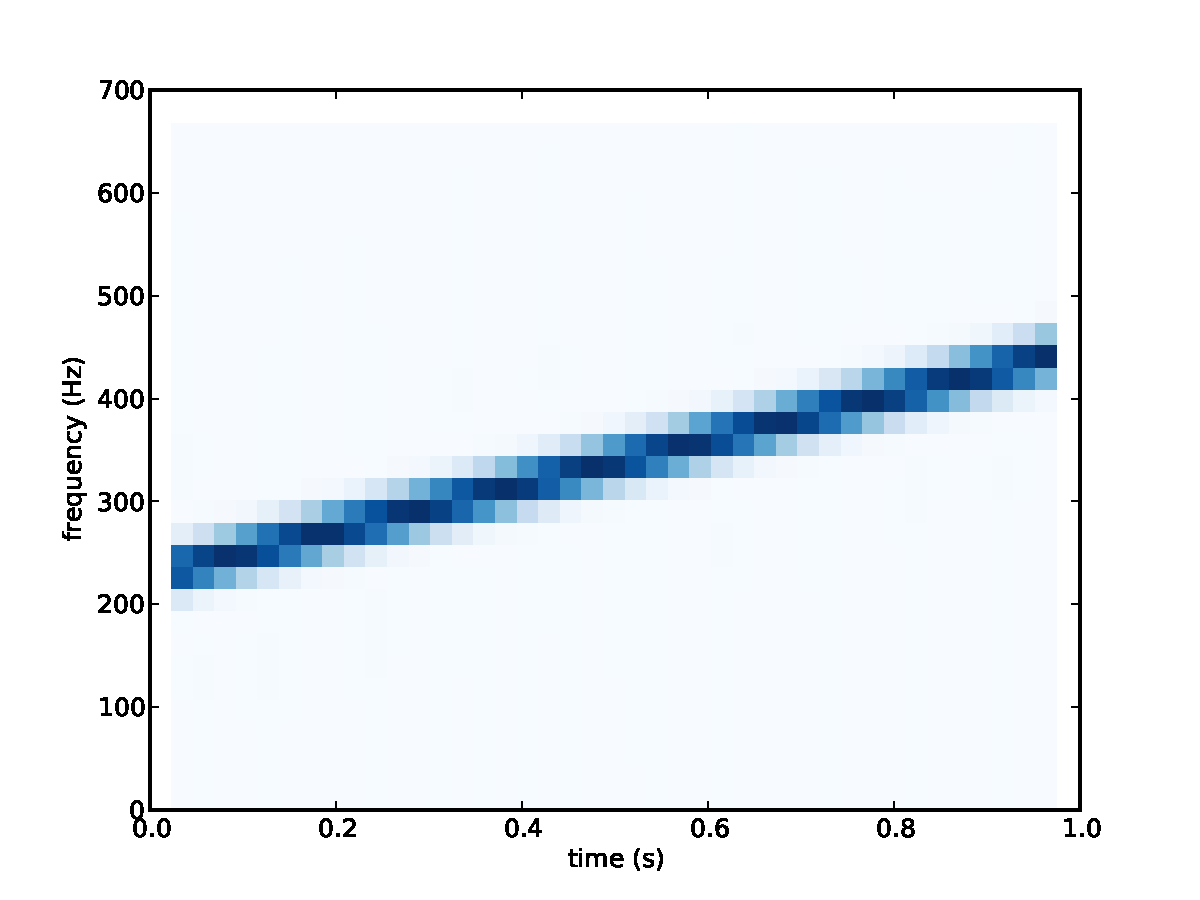
\includegraphics[height=2.5in]{figs/chirp2.pdf}}
\caption{Spectrogram of a one-second one-octave chirp.}
\label{fig.chirp2}
\end{figure}

To recover the relationship between frequency and time, we can break
the chirp into segments and plot the spectrum of each segment.  The
result is called a {\bf short-time Fourier transform} (STFT).

There are several ways to visualize a STFT, but the most common
is a {\bf spectrogram}, which shows time on the x-axis and frequency
on the y-axis.  Each column in the spectrogram shows the spectrum of
a short segment, using color or grayscale to represent amplitude.

{\tt Wave} provides \verb"make_spectrogram", which returns a
{\tt Spectrogram} object:

\begin{verbatim}
    signal = thinkdsp.Chirp(start=220, end=440)
    wave = signal.make_wave(duration=1)
    spectrogram = wave.make_spectrogram(seg_length=512)
    spectrogram.plot(high=32)
\end{verbatim}

\verb"seg_length" is the number of samples in each segment.  I chose
512 because FFT is most efficient when the number of samples is a
power of 2.

Figure~\ref{fig.chirp2} shows the result.  The x-axis shows time from
0 to 1 seconds.  The y-axis shows frequency from 0 to 700 Hz.  I cut
off the top part of the spectrogram; the full range goes to 5012.5 Hz,
which is half of the framerate.

The spectrogram shows clearly that frequency increases linearly
over time.  Similarly, in the spectrogram of an exponential chirp, we
can see the shape of the exponential curve.

However, notice that the peak in each column is blurred across 2--3
cells.  This blurring reflects the limited resolution of the
spectrogram.


\section{The Gabor limit}
\label{gabor}

The {\bf time resolution} of the spectrogram is the duration of the
segments, which corresponds to the width of the cells in the
spectrogram.  Since each segment is 512 frames, and there are 11,025
frames per second, there are 0.046 seconds per segment.

The {\bf frequency resolution} is the frequency range between
elements in the spectrum, which corresponds to the height of the
cells.  With 512 frames, we get 256 frequency components over a range
from 0 to 5012.5 Hz, so the range between components is 21.5 Hz.

More generally, if $n$ is the segment length, the spectrum contains
$n/2$ components.  If the framerate is $r$, the maximum frequency in
the spectrum is $r/2$.  So the time resolution is $n/r$ and the
frequency resolution is
%
\[ \frac{r/2}{n/2} \]
%
which is $r/n$.

Ideally we would like time resolution to be small, so we can see rapid
changes in frequency.  And we would like frequency resolution to be
small so we can see small changes in frequency.  But you can't have
both.  Notice that time resolution, $n/r$, is the inverse of frequency
resolution, $r/n$.  So if one gets smaller, the other gets bigger.

For example, if you double the segment length, you cut frequency
resolution in half (which is good), but you double time resolution
(which is bad).  Even increasing the framerate doesn't help.  You get
more samples, but the range of frequencies increases at
the same time.

This tradeoff is called the ``Gabor limit'' and it is a fundamental
limitation of this kind of time-frequency analysis.


\section{Implementing spectrograms}

\begin{figure}
% chirp.py
\centerline{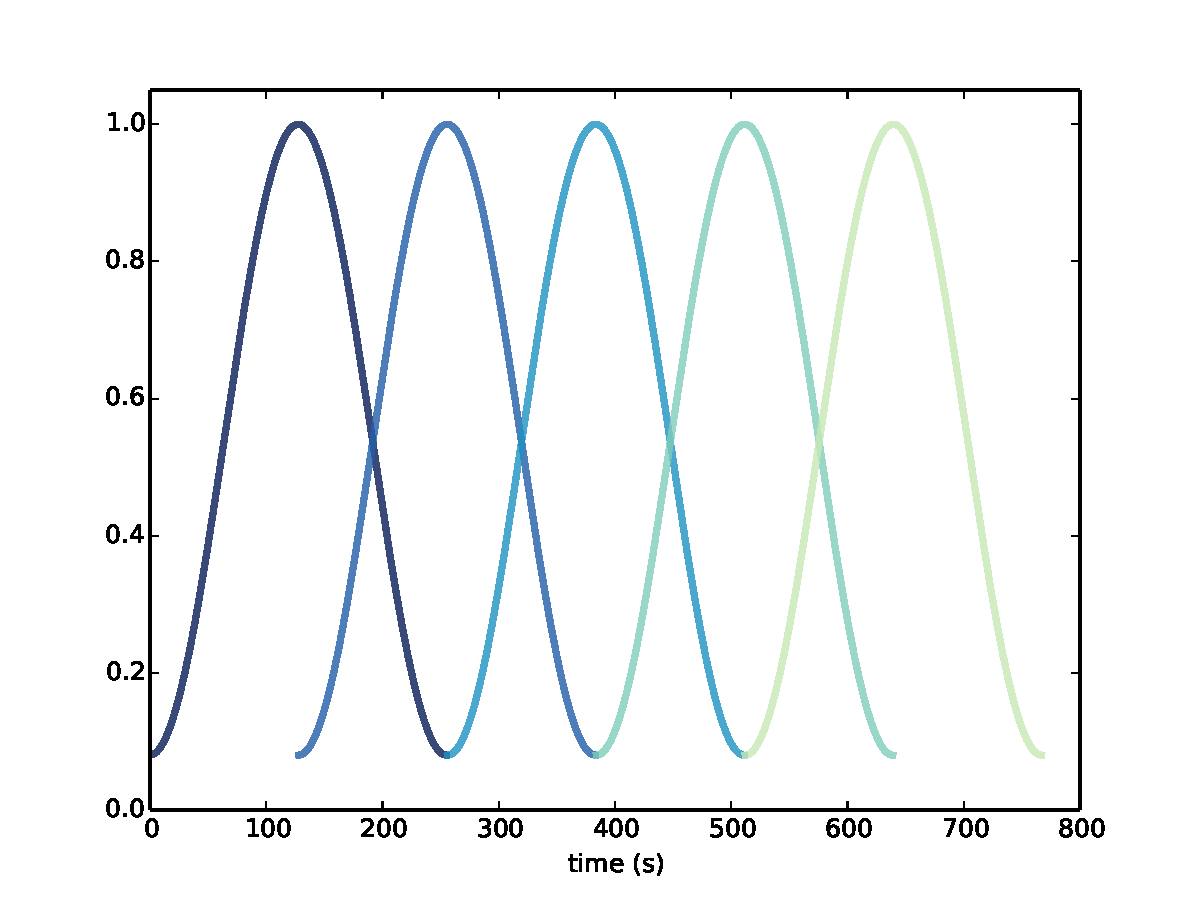
\includegraphics[height=2.5in]{figs/windowing3.pdf}}
\caption{Overlapping Hamming windows.}
\label{fig.windowing3}
\end{figure}

Here is the {\tt Wave} method that computes spectrograms:

\begin{verbatim}
    def make_spectrogram(self, seg_length):
        n = len(self.ys)
        window = numpy.hamming(seg_length)

        start, end, step = 0, seg_length, seg_length / 2
        spec_map = {}

        while end < n:
            ys = self.ys[start:end] * window
            hs = numpy.fft.rfft(ys)

            t = (start + end) / 2.0 / self.framerate
            spec_map[t] = Spectrum(hs, self.framerate)

            start += step
            end += step

        return Spectrogram(spec_map, seg_length)
\end{verbatim}

\verb"seg_length" is the number of samples in each segment.
{\tt n} is the number of samples in the wave.  {\tt window}
is a Hamming window with the same length as the segments.

{\tt start} and {\tt end} are the slice indices that select
the segments from the wave.  {\tt step} is the offset between
segments.  Since {\tt step} is half of \verb"seg_length", the
segments overlap by half.  Figure~\ref{fig.windowing3} shows what
these overlapping windows look like.

Inside the while loop, we select a slice from the wave, multiply
by the window, and compute the FFT.  Then we construct a Spectrum
object and add it to \verb"spec_map" which is a map from the
midpoint of the segment in time to the Spectrum object.

Finally, the method constructs and returns a Spectrogram.  Here
is the definition of Spectrogram:

\begin{verbatim}
class Spectrogram(object):

    def __init__(self, spec_map, seg_length):
        self.spec_map = spec_map
        self.seg_length = seg_length
\end{verbatim}

Like many \verb"__init__" methods, this one just stores the
parameters as attributes.

{\tt Spectrogram} provides {\tt plot}, which generates a
pseudocolor plot:

\begin{verbatim}
    def plot(self, low=0, high=None):
        ts = self.times()
        fs = self.frequencies()[low:high]

        # copy amplitude from each spectrum into a column of the array
        size = len(fs), len(ts)
        array = numpy.zeros(size, dtype=numpy.float)

        # copy each spectrum into a column of the array
        for i, t in enumerate(ts):
            spectrum = self.spec_map[t]
            array[:,i] = spectrum.amps[low:high]

        thinkplot.pcolor(ts, fs, array)
\end{verbatim}

{\tt plot} uses {\tt times}, which the returns the midpoint of each
time segment in a sorted sequence, and {\tt frequencies}, which returns
the frequencies of the components in the spectrums.

{\tt array} is a numpy array that holds the amplitudes from the
spectrums, with one column for each point in time and one row
for each frequency.  The {\tt for} loop iterates through the times
and copies the amplitudes from each spectrum into a column of the array.

Finally {\tt thinkplot.pcolor} is a wrapper around {\tt pyplot.pcolor},
which generates the pseudocolor plot.

And that's how Spectrograms are implemented.


\section{Exercises}

\begin{exercise}
Run and listen to the examples in {\tt chap03.ipynb}, which is
in the repository for this book, and also available at
\url{http://tinyurl.com/thinkdsp03}.

In the leakage example, try replacing the Hamming window with one of
the other windows provided by NumPy, and see what effect they have on
leakage.  See
\url{http://docs.scipy.org/doc/numpy/reference/routines.window.html}
\end{exercise}

\begin{exercise}
Write a class called {\tt SawtoothChirp} that extends {\tt Chirp}
and overrides {\tt evaluate} to generate a sawtooth waveform with
frequency that increases (or decreases) linearly.

Hint: combine the evaluate functions from {\tt Chirp} and {\tt
  SawtoothSignal}.

Draw a sketch of what you think the spectrogram of this signal
looks like, and then plot it.  The effect of aliasing should be
visually apparent, and if you listen carefully, you can hear it.
\end{exercise}


\begin{exercise}
Another way to generate a sawtooth chirp is to add up a harmonic
series of sinusoidal chirps.  Write another version of {\tt
  SawtoothChirp} that uses this method and plot the spectrogram.
\end{exercise}

\begin{exercise}
In musical terminology, a ``glissando'' is a note that slides from one
pitch to another, so it is similar to a chirp.  A trombone player can
play a glissando by extending the trombone slide while blowing
continuously.  As the slide extends, the total length of the tube gets
longer, and the resulting pitch is inversely proportional to length.

Assuming that the player moves the slide at a constant speed, how
does frequency vary with time?  Is a trombone glissando more like
a linear or exponential chirp?

Write a function that simulates a trombone glissando from C3 up to F3
and back down to C3.  C3 is 262 Hz; F3 is 349 Hz.
\end{exercise}


\begin{exercise}
George Gershwin's {\it Rhapsody in Blue} starts with a famous
clarinet glissando.  Find a recording of this piece and plot
a spectrogram of the first few seconds.

% http://archive.org/details/rhapblue11924
\end{exercise}

\begin{exercise}
Make or find a recording of a series of vowel sounds and look at the
spectrogram.  Can you identify different vowels?
\end{exercise}



\chapter{Noise}

In English, ``noise'' means an unwanted or unpleasant sound.  In the
context of digital signal processing, it has two different senses:

\begin{enumerate}

\item As in English, it can mean an unwanted signal of any kind.  If
two signals interfere with each other, each signal would consider
the other to be noise.

\item ``Noise'' also refers to a signal that contains components at
many frequencies, so it lacks the harmonic structure of the periodic
signals we saw in previous chapters.  

\end{enumerate}

The code for this chapter is in {\tt noise.py}, which is in the
repository for this book (see Section~\ref{code}).  You can listen
to the examples in {\tt chap04.ipynb}, which you can view at
\url{http://tinyurl.com/thinkdsp04}.

\section{Uncorrelated noise}

\begin{figure}
% noise.py
\centerline{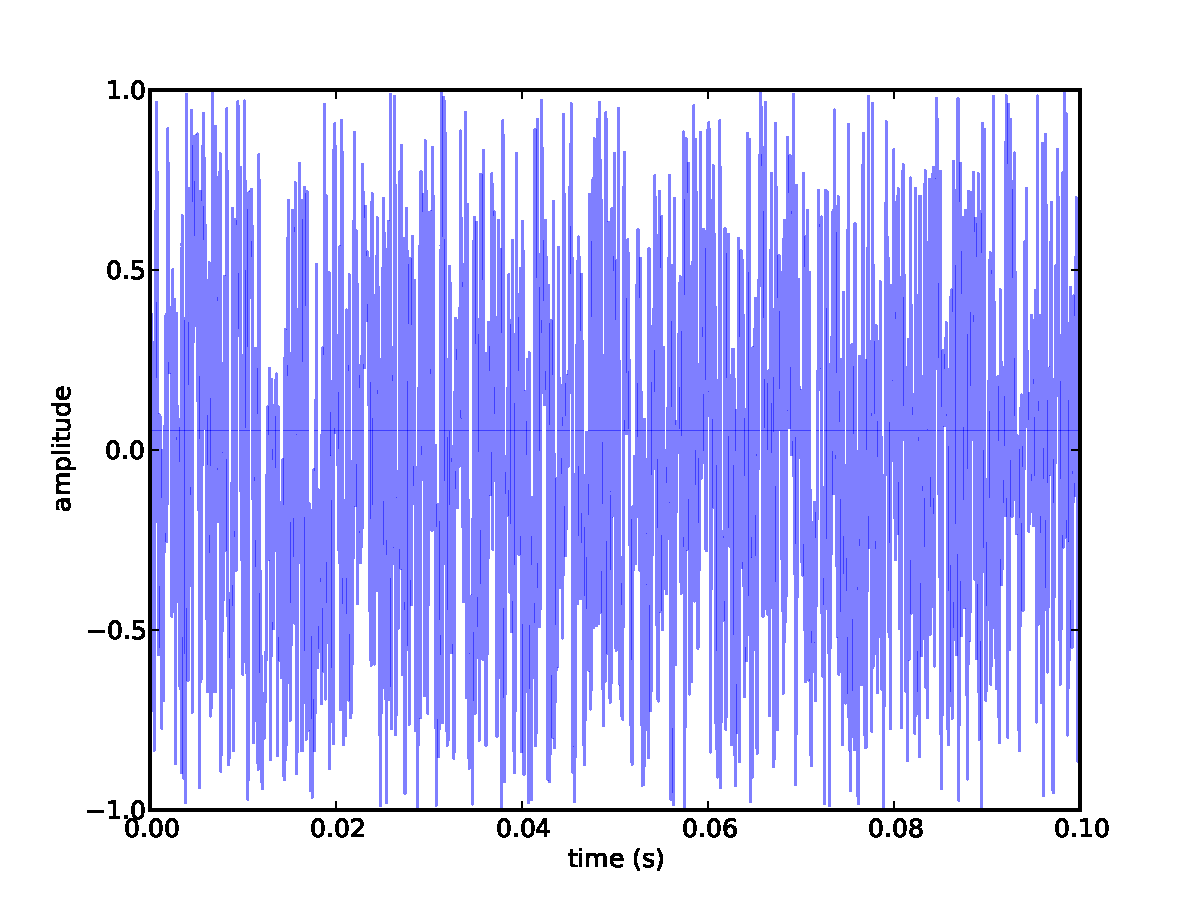
\includegraphics[height=2.5in]{figs/whitenoise0.pdf}}
\caption{Waveform of uncorrelated uniform noise.}
\label{fig.whitenoise0}
\end{figure}

The simplest way to understand noise is to generate it, and the
simplest kind to generate is uncorrelated uniform noise (UU noise).
``Uniform'' means the signal contains random values from a uniform
distribution; that is, every value in the range is equally likely.
``Uncorrelated'' means that the values are independent; that is,
knowing one value provides no information about the others.

This code generates UU noise:

\begin{verbatim}
    duration = 0.5
    framerate = 11025
    n = framerate * duration
    ys = numpy.random.uniform(-1, 1, n)
    wave = thinkdsp.Wave(ys, framerate)
    wave.plot()
\end{verbatim}

The result is a wave with duration 0.5 seconds at 11,025
samples per second.  Each sample is drawn from a uniform distribution
between -1 and 1.

If you play this wave, it sounds like the static you hear if you tune
a radio between channels.  Figure~\ref{fig.whitenoise0} shows what the
waveform looks like.  As expected, it looks pretty random.

\begin{figure}
% noise.py
\centerline{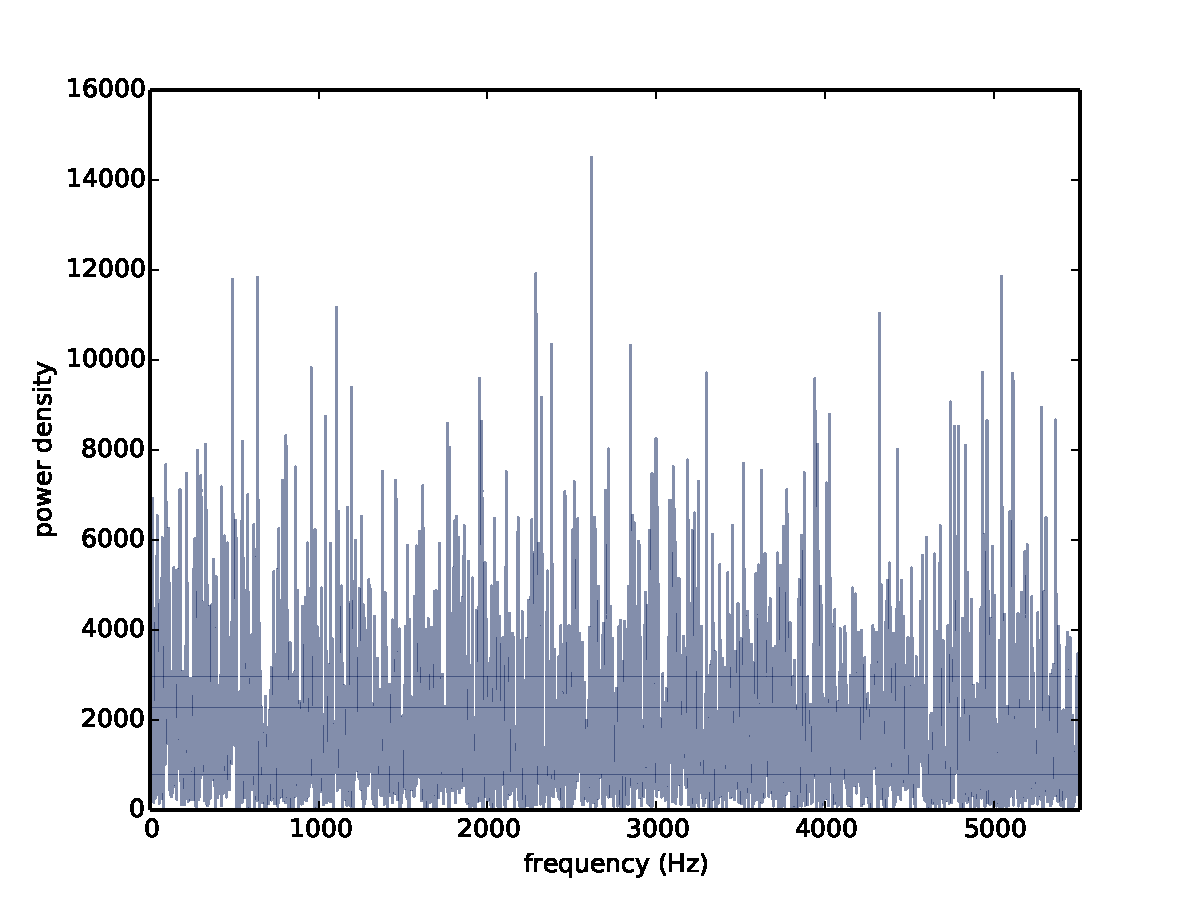
\includegraphics[height=2.5in]{figs/whitenoise1.pdf}}
\caption{Spectrum of uncorrelated uniform noise.}
\label{fig.whitenoise1}
\end{figure}

Now let's take a look at the spectrum:

\begin{verbatim}
    spectrum = wave.make_spectrum()
    spectrum.plot_power()
\end{verbatim}

\verb"Spectrum.plot_power" is similar to \verb"Spectrum.plot",
except that it plots power density instead of amplitude.  Power 
density is the square of amplitude, expressed in units of power per Hz.
(I am switching from amplitude to power in this section because
it is more conventional in the context of noise.)

Figure~\ref{fig.whitenoise1} shows the result.  Like the signal, the
spectrum looks pretty random.  And it is, but we have to be more
precise about the word ``random.''  There are at least three things we
might like to know about a noise signal or its spectrum:

\begin{itemize}

\item Distribution: The distribution of a random signal is the set of
  possible values and their probabilities.  For example, in the
  uniform noise signal, the set of values is the range from -1 to 1,
  and all values have the same probability.  An alternative is
  {\bf Gaussian noise}, where the set of values is the range from negative
  to positive infinity, but values near 0 are the most likely, with
  probability that drops off according to the Gaussian or
  ``bell'' curve.

\item Correlation: Is each value in the signal independent of the
  others, or are there dependencies between them?  In UU noise, the
  values are independent.
  An alternative is {\bf Brownian noise}, where each value is the sum
  of the previous value and a random ``step''.  So if the value of the
  signal is high at a particular point in time, we expect it to stay
  high, and if it is low, we expect
  it to stay low.

\item Relationship between power and frequency: In the spectrum of UU
  noise, the power at all frequencies is drawn from the same
  distribution; that is, there is no relationship between power and
  frequency (or, if you like, the relationship is a constant).  An
  alternative is {\bf pink noise}, where power is inversely related
  to frequency; that is, the power at frequency $f$ is drawn from
  a distribution whose mean is proportional to $1/f$.

\end{itemize}


\section{Integrated spectrum}

For UU noise we can see the relationship between power and frequency
more clearly by looking at the {\bf integrated spectrum}, which
is a function of frequency, $f$, that shows the cumulative total power in
the spectrum up to $f$.

\begin{figure}
% noise.py
\centerline{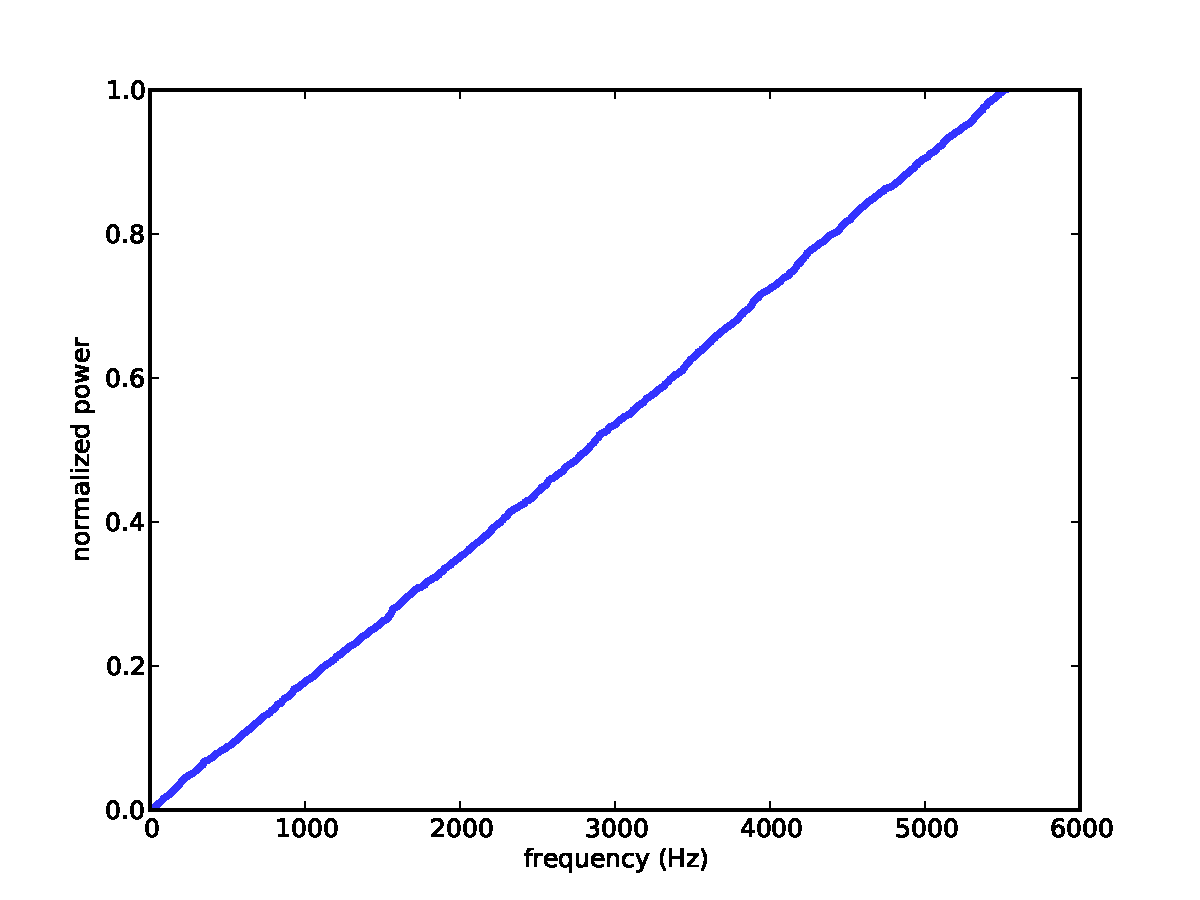
\includegraphics[height=2.5in]{figs/whitenoise2.pdf}}
\caption{Integrated spectrum of uncorrelated uniform noise.}
\label{fig.whitenoise2}
\end{figure}

{\tt Spectrum} provides a method that computes the IntegratedSpectrum:

\begin{verbatim}
    def make_integrated_spectrum(self):
        cs = numpy.cumsum(self.power)
        cs /= cs[-1]
        return IntegratedSpectrum(cs, self.fs)
\end{verbatim}

{\tt self.power} is a NumPy array containing power for each frequency.
{\tt numpy.cumsum} computes the cumulative sum of the powers.
Dividing through by the last element normalizes the integrated
spectrum so it runs from 0 to 1.

The result is an IntegratedSpectrum.  Here is the class definition:

\begin{verbatim}
class IntegratedSpectrum(object):    
    def __init__(self, cs, fs):
        self.cs = cs
        self.fs = fs
\end{verbatim}

Like Spectrum, IntegratedSpectrum provides \verb"plot_power", so
we can compute and plot the integrated spectrum like this:

\begin{verbatim}
    integ = spectrum.make_integrated_spectrum()
    integ.plot_power()
    thinkplot.show(xlabel='frequency (Hz)',
                   ylabel='cumulative power')
\end{verbatim}

The result, shown in Figure~\ref{fig.whitenoise2}, is a straight line,
which indicates that power at all frequencies is constant, on average.
Noise with equal power at all frequencies is called {\bf white noise}
by analogy with light, because an equal mixture of light at all
visible frequencies is white.



\section{Brownian noise}

\begin{figure}
% noise.py
\centerline{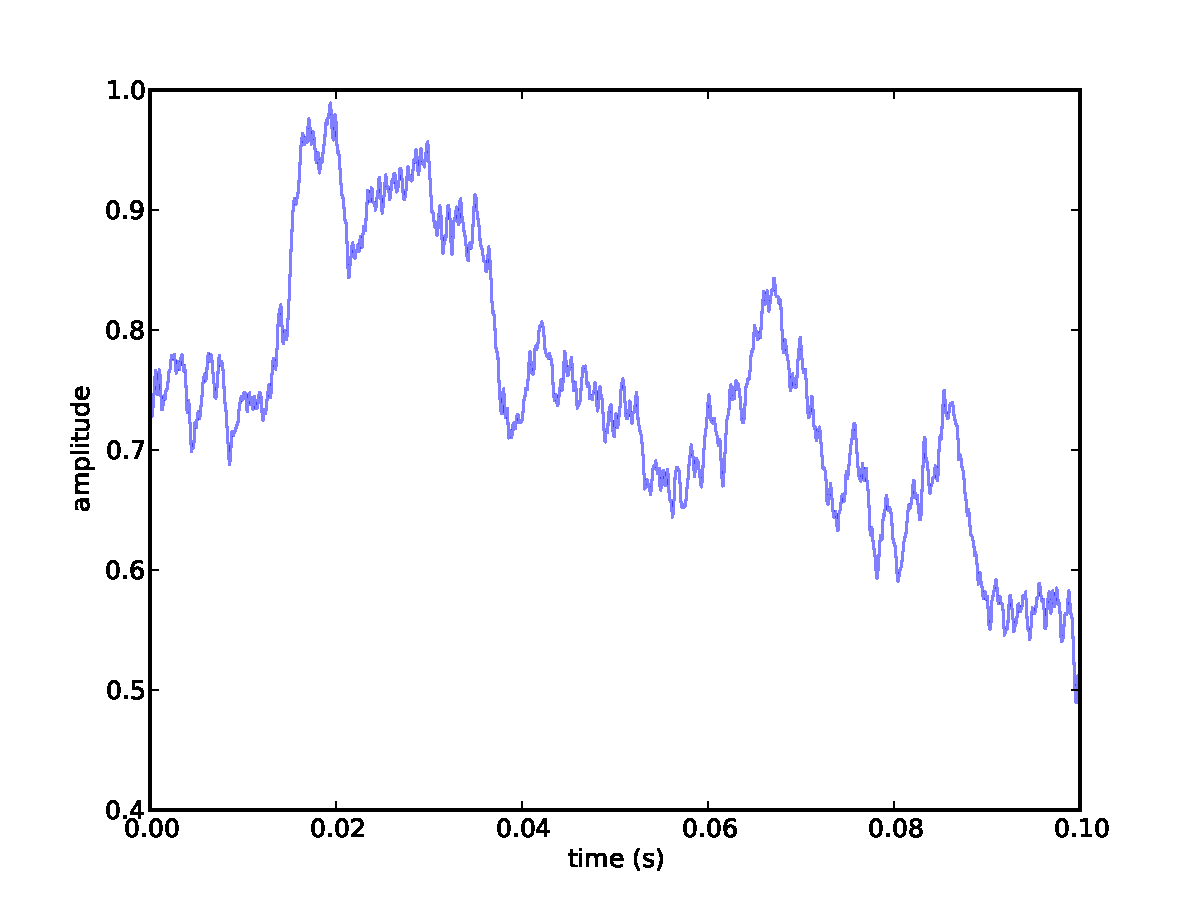
\includegraphics[height=2.5in]{figs/rednoise0.pdf}}
\caption{Waveform of Brownian noise.}
\label{fig.rednoise0}
\end{figure}

UU noise is uncorrelated, which means that each value does not depend
on the others.  An alternative is Brownian noise, in which each value
is the sum of the previous value and a random ``step''.

It is called ``Brownian'' by analogy with Brownian motion, in which a
particle suspended in a fluid moves apparently at random, due to
unseen interactions with the fluid.  Brownian motion is often
described using a {\bf random walk}, which is a mathematical model 
of a path where the distance between steps is characterized by a
random distribution.

In a one-dimensional random walk, the particle moves up or down
by a random amount at each time step.  The location of the particle
at any point in time is the sum of all previous steps.

This observation suggests a way to generate Brownian noise:
generate uncorrelated random steps and then add them up.
Here is a class definition that implements this algorithm:

\begin{verbatim}
class BrownianNoise(_Noise):

    def evaluate(self, ts):
        dys = numpy.random.uniform(-1, 1, len(ts))
        ys = numpy.cumsum(dys)
        ys = normalize(unbias(ys), self.amp)
        return ys
\end{verbatim}

We use {\tt numpy.random.uniform} to generate an uncorrelated signal
and {\tt numpy.cumsum} to compute their cumulative sum.

Since the sum is likely to escape the range from -1 to
1, we have to use {\tt unbias} to shift the mean to 0, and {\tt
  normalize} to get the desired maximum amplitude.

Here's the code that generates a BrownianNoise object and plots the
waveform.

\begin{verbatim}
    signal = thinkdsp.BrownianNoise()
    wave = signal.make_wave(duration=0.5, framerate=11025)
    wave.plot()
\end{verbatim}

Figure~\ref{fig.rednoise0} shows the result.  The waveform
wanders up and down, but there is a clear correlation between
successive values.  When the amplitude is high, it tends to stay
high, and vice versa.

\begin{figure}
% noise.py
\centerline{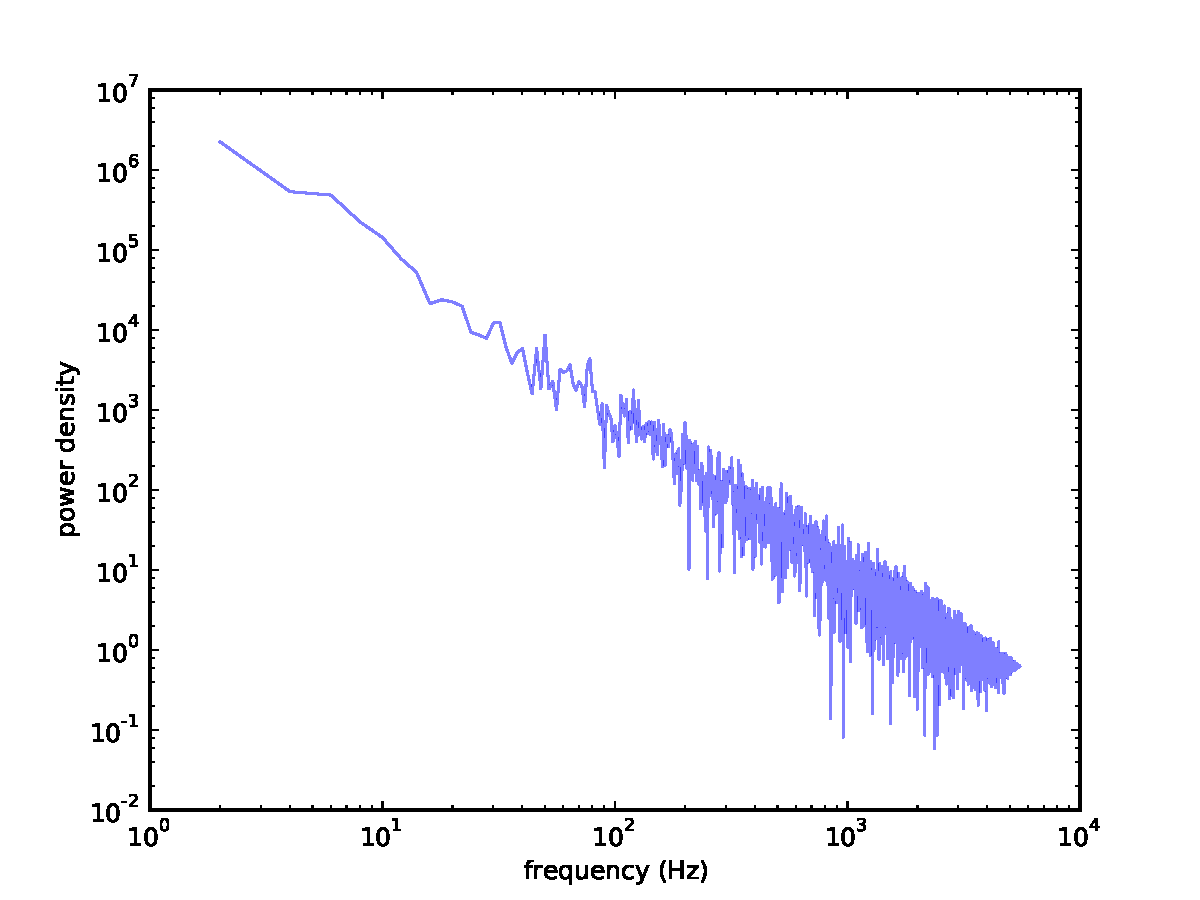
\includegraphics[height=2.5in]{figs/rednoise3.pdf}}
\caption{Spectrum of Brownian noise on a log-log scale.}
\label{fig.rednoise3}
\end{figure}

If you plot the spectrum of Brownian noise, it doesn't look like
much.  Nearly all of the power is at the lowest frequencies; on a
linear scale, the higher frequency components are not visible.

To see the shape of the spectrum, we have to plot power density
and frequency on a log-log scale.  Here's the code:

\begin{verbatim}
    spectrum = wave.make_spectrum()
    spectrum.plot_power(low=1, linewidth=1, alpha=0.5)
    thinkplot.show(xlabel='frequency (Hz)',
                   ylabel='power density',
                   xscale='log',
                   yscale='log')
\end{verbatim}

The slope of this line is approximately -2 (we'll see why in
Chapter~\ref{systems}), so we can write this relationship:
%
\[ \log P = k -2 \log f \]
%
where $P$ is power, $f$ is frequency, and $k$ is the intercept
of the line (which is not relevant for our purposes).
Exponentiating both sides yields:
%
\[ P = K / f^{2} \]
%
where $K$ is $e^k$, but still not relevant.  More important is
that power is proportional to $1/f^2$, which is characteristic
of Brownian noise.

Brownian noise is also called ``red noise,'' for the same reason that
white noise is called ``white.''  If you combine visible light with
the same relationship between frequency and power, most of the power
would be at the low-frequency end of the spectrum, which is red.
Brownian noise is also sometimes called ``brown noise'', but I think
that's confusing, so I won't use it.


\section{Pink Noise}
\label{pink}

\begin{figure}
% noise.py
\centerline{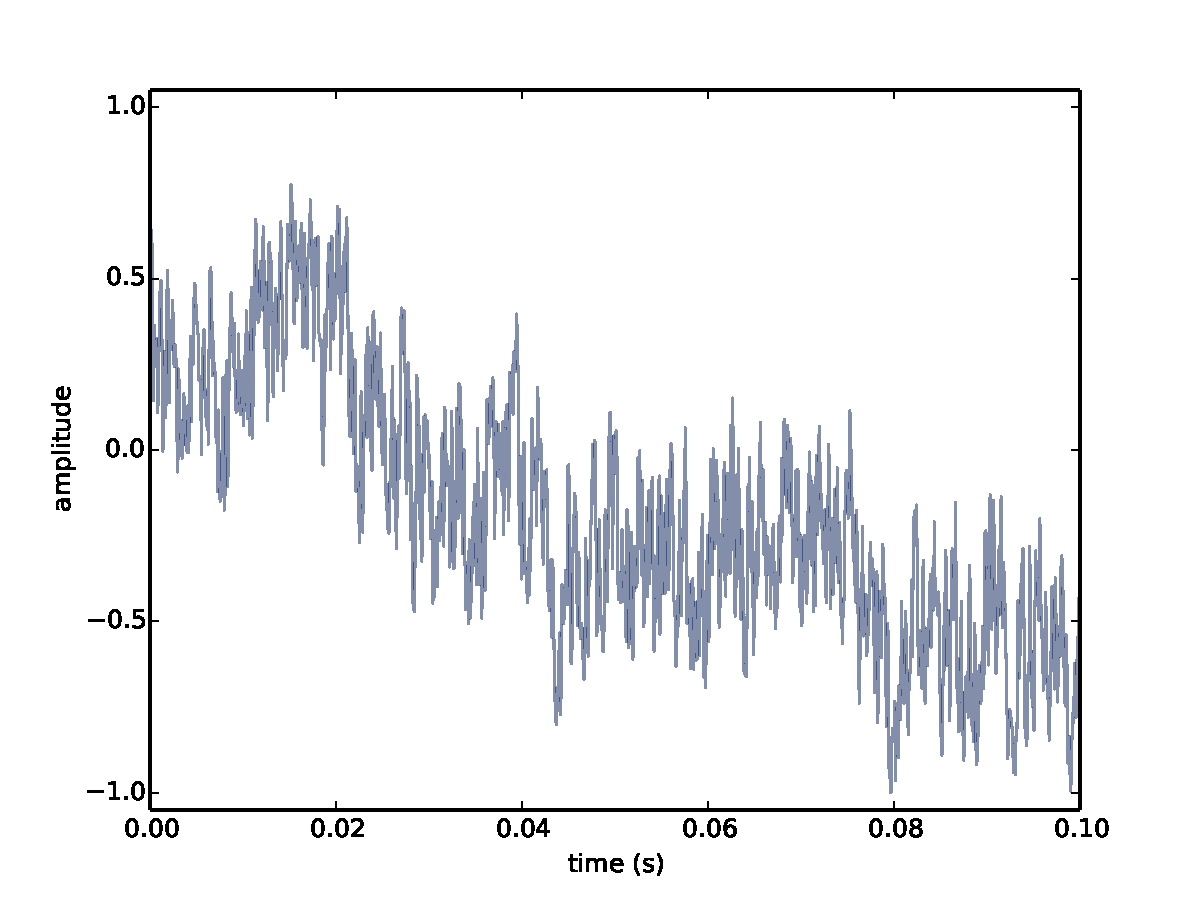
\includegraphics[height=2.5in]{figs/pinknoise0.pdf}}
\caption{Waveform of pink noise with $\beta=1$.}
\label{fig.pinknoise0}
\end{figure}

For red noise, the relationship between frequency
and power is
%
\[ P = K / f^{2} \]
%
There is nothing special about the exponent -2.  More generally,
we can synthesize noise with any exponent, $\beta$.
%
\[ P = K / f^{\beta} \]
%
When $\beta = 0$, power is constant at all frequencies,
so the result is white noise.  When $\beta=2$ the result is red noise.

When $\beta$ is between 0 and 2, the result is between white and
red noise, so it is called ``pink noise''

There are several ways to generate pink noise.  The simplest is to
generate white noise and then apply a low-pass filter with the
desired exponent.  {\tt thinkdsp} provides a class that represents
a pink noise signal:

\begin{verbatim}
class PinkNoise(_Noise):

    def __init__(self, amp=1.0, beta=1.0):
        self.amp = amp
        self.beta = beta
\end{verbatim}

{\tt amp} is the desired amplitude of the signal.
{\tt beta} is the desired exponent.  {\tt PinkNoise} provides
\verb"make_wave", which generates a Wave.

\begin{verbatim}
    def make_wave(self, duration=1, start=0, framerate=11025):
        signal = UncorrelatedUniformNoise()
        wave = signal.make_wave(duration, start, framerate)
        spectrum = wave.make_spectrum()

        spectrum.pink_filter(beta=self.beta)

        wave2 = spectrum.make_wave()
        wave2.unbias()
        wave2.normalize()
        return wave2
\end{verbatim}

{\tt duration} is the length of the wave in seconds.  {\tt start} is
the start time of the wave, which is included so that \verb"make_wave"
has the same interface for all types of noise, but for random noises,
start time is irrelevant.  And {\tt framerate} is the number of
samples per second.

\begin{figure}
% noise.py
\centerline{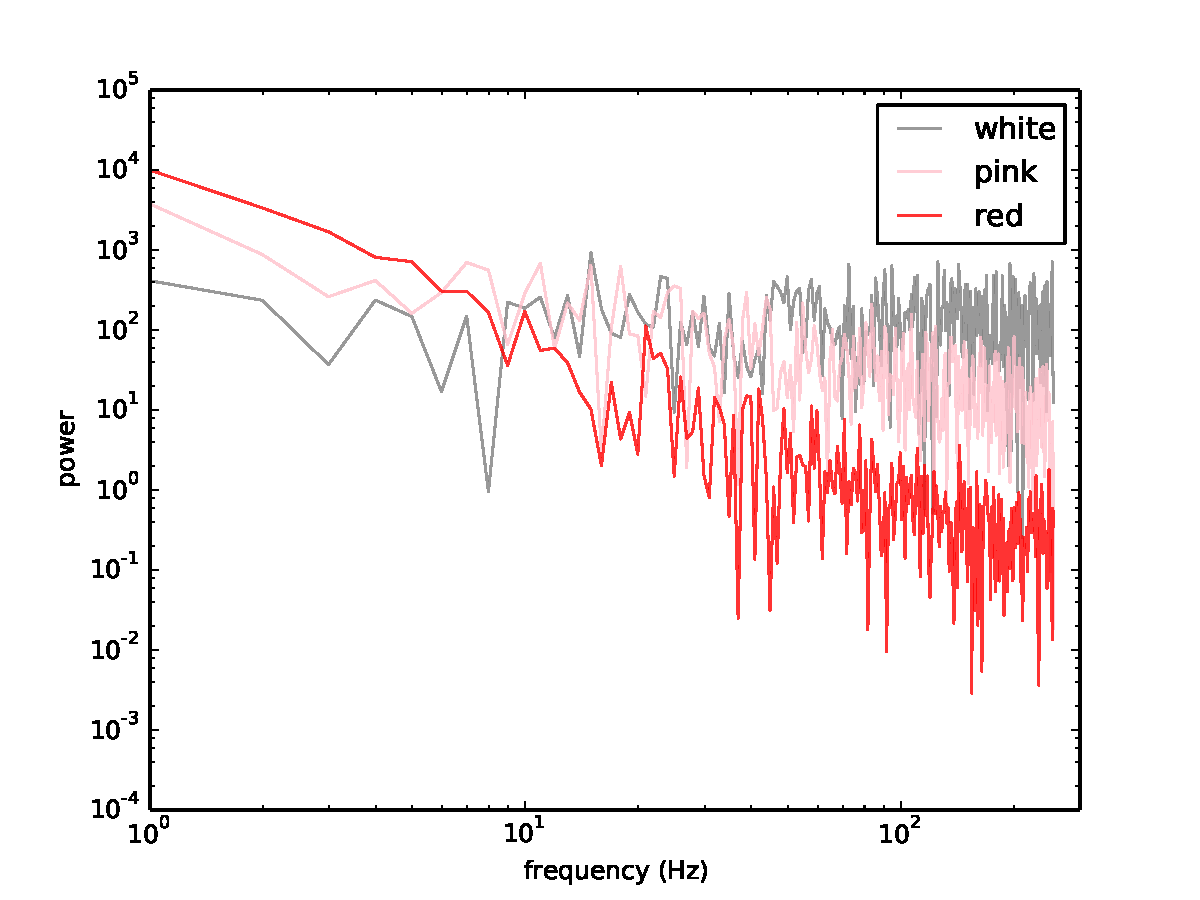
\includegraphics[height=2.5in]{figs/noise-triple.pdf}}
\caption{Spectrum of white, pink, and red noise on a log-log scale.}
\label{fig.noise-triple}
\end{figure}

\verb"make_wave" creates a white noise wave, computes its spectrum,
applies a filter with the desired exponent, and then converts the
filtered spectrum back to a wave.  Then it unbiases and normalizes
the wave.

{\tt Spectrum} provides \verb"pink_filter":

\begin{verbatim}
    def pink_filter(self, beta=1.0):
        denom = self.fs ** (beta/2.0)
        denom[0] = 1
        self.hs /= denom
\end{verbatim}

\verb"pink_filter" divides each element of the spectrum by
$f^{\beta/2}$.  Since power is the square of amplitude, this
operation divides the power at
each component by $f^\beta$.  It treats the component
at $f=0$ as a special case, partly to avoid dividing by 0, but
also because this element represents the bias of the signal,
which we are going to set to 0 anyway. 

Figure~\ref{fig.pinknoise0} shows the resulting waveform.  Like
Brownian noise, it wanders up and down in a way that suggests
correlation between successive values, but at least visually, it looks
more random.  In the next chapter we will come back to this
observation and I will be more precise about what I mean by
``correlation'' and ``more random.''

Finally, Figure~\ref{fig.noise-triple} shows a spectrum for
white, pink, and red noise on the same log-log scale.
The relationship between the exponent, $\beta$, and the slope
of the spectrum is apparent in this figure.


\section{Gaussian noise}

\begin{figure}
% noise.py
\centerline{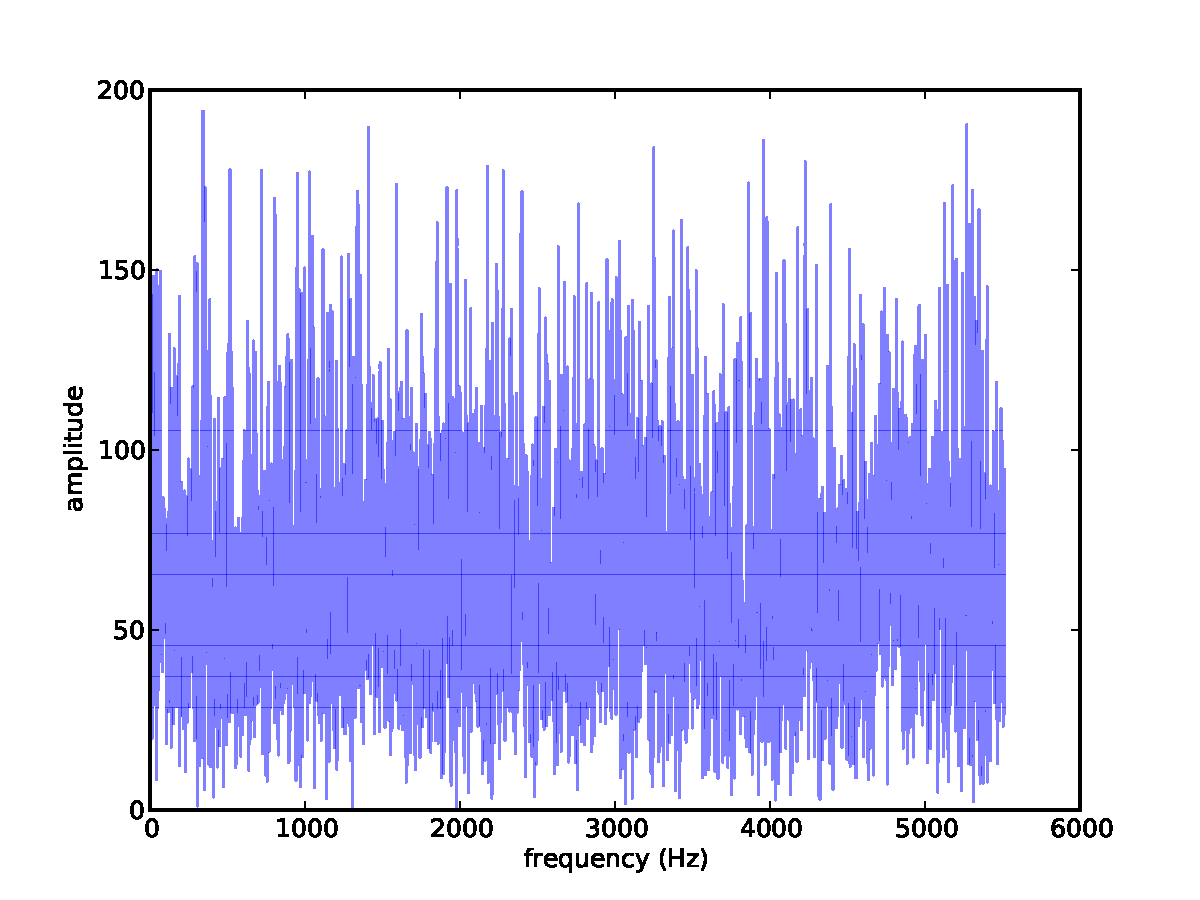
\includegraphics[height=2.5in]{figs/noise1.pdf}}
\caption{Normal probability plot for the real and imaginary parts
of the spectrum of Gaussian noise.}
\label{fig.noise1}
\end{figure}

We started with uncorrelated uniform (UU) noise and showed that,
because its spectrum has equal power at all frequencies, on
average, UU noise is white.

But when people talk about ``white noise'', they don't always
mean UU noise.  In fact, more often they mean uncorrelated
Gaussian (UG) noise.

{\tt thinkdsp} provides an implementation of UG noise:

\begin{verbatim}
class UncorrelatedGaussianNoise(_Noise):

    def evaluate(self, ts):
        ys = numpy.random.normal(0, self.amp, len(ts))
        return ys
\end{verbatim}

{\tt numpy.random.normal} returns a NumPy array of values from a
Gaussian distribution, in this case with mean 0 and standard deviation
{\tt self.amp}.  In theory the range of values is from negative to
positive infinity, but we expect about 99\% of the values to be
between -3 and 3.

UG noise is similar in many ways to UU noise.  The spectrum has
equal power at all frequencies, on average, so UG is also white.
And it has one other interesting property: the spectrum of UG
noise is also UG noise.  More precisely, the real and imaginary
parts of the spectrum are uncorrelated Gaussian values.

To test that claim, we can generate the spectrum of UG noise and
then generate a ``normal probability plot,'' which is a graphical
way to test whether a distribution is Gaussian.

\begin{verbatim}
    signal = thinkdsp.UncorrelatedGaussianNoise()
    wave = signal.make_wave(duration=0.5, framerate=11025)
    spectrum = wave.make_spectrum()

    thinkstats2.NormalProbabilityPlot(spectrum.real)
    thinkstats2.NormalProbabilityPlot(spectrum.imag)
\end{verbatim}

{\tt NormalProbabilityPlot} is provided by {\tt thinkstats2}, which is
included in the repository for this book.  If you are not familiar
with normal probability plots, you can read about them in
{\it Think Stats} at \url{http://thinkstats2.com}.

Figure~\ref{fig.noise1} shows the results.  The gray lines
show a linear model fit to the data; the dark lines show the
data.

A straight line on a normal probability plot indicates
that the data come from a Gaussian distribution.  Except for
some random variation at the extremes, these lines are straight,
which indicates that the spectrum of UG noise is UG noise.

The spectrum of UU noise is also UG noise, at least approximately.  In
fact, by the Central Limit Theorem, the spectrum of almost any
uncorrelated noise is approximately Gaussian, as long as the
distribution has finite mean and standard deviation and the number of
samples is large.


\section{Exercises}

\begin{exercise}
The algorithm in this chapter for generating pink noise is
conceptually simple but computationally expensive.  There are
more efficient alternatives, like the Voss-McCartney algorithm.
Research this method, implement it, compute the spectrum of
the result, and confirm that it has the desired relationship
between power and frequency.
\end{exercise}


\begin{exercise}
``A Soft Murmur'' is a web site that plays a mixture of natural
noise sources, including rain, waves, wind, etc.  At
\url{http://asoftmurmur.com/about/} you can find their list
of recordings, most of which are at \url{http://freesound.org}.

Download a few of these files and compute the spectrum of each
signal.  Does the power spectrum look like white noise, pink noise,
or Brownian noise?  How does the spectrum vary over time?
\end{exercise}


\begin{exercise}
%TODO: make this part of the text?

In a white noise signal, the mixture of frequencies changes over time.
In the long run, we expect the power at all frequencies to be equal,
but in any sample, the power at each frequency is random.

To estimate the long-term average power at each frequency, we can
break a long signal into segments, compute the power spectral
density for each segment, and then compute the average across
the segments.  You can read more about this algorithm at
\url{http://en.wikipedia.org/wiki/Bartlett's_method}.

At \url{http://www.coindesk.com} you can download the daily
price of a BitCoin as a CSV file.  Read this file and compute
the power spectrum of BitCoin prices as a function of time.
Does it resemble white, pink, or Brownian noise?
\end{exercise}



\chapter{Autocorrelation}

In the previous chapter I characterized white noise as ``uncorrelated'',
which means that each value is independent of the others, and Brownian
noise as ``correlated'', because each value depends on the preceding
value.  In this chapter I define these terms more precisely and
present the {\bf autocorrelation function}, which is a useful tool
for signal analysis.

But before we get to autocorrelation, let's start with correlation.

The code for this chapter is in {\tt autocorr.py}, which is in the
repository for this book (see Section~\ref{code}).


\section{Correlation}

In general, correlation between variables means that if you know the
value of one, you have some information about the other.  There are
several ways to quantify correlation, but the most common is the
Pearson product-moment correlation coefficient, usually denoted
$\rho$.  For two variables, $x$ and $y$, that each contain $N$ values:
%
\[ \rho = \frac{ \sum_i (x_i - \mu_x) (y_i - \mu_y)}{N \sigma_x \sigma_y} \]
%
Where $\mu_x$ and $\mu_y$ are the means of $x$ and $y$, and
$\sigma_x$ and $\sigma_y$ are their standard deviations.

Pearson's correlation is always between -1 and +1 (including both).
If $\rho$ is positive, we say that the correlation is positive,
which means that when one variable is high, the other tends to be
high.  If $\rho$ is negative, the correlation is negative, so
when one variable is high, the other is low.

The magnitude of $\rho$ indicates the strength of the correlation.  If
$\rho$ is 1 or -1, the variables are perfectly correlated, which means
that if you know one, you can make a perfect prediction about the
other.

If $\rho$ is near zero, the correlation might be weak, or there might
be a nonlinear relationship that is not captured by this coefficient
of correlation.  Nonlinear relationships are often important in
statistics, but less often relevant for signal processing, so I
won't say more about them here.

In the context of signal processing, we are often working with
unbiased signals, where the mean is 0, and normalized signals, where the
standard deviation is 1.  In that case, the definition of $\rho$
simplifies to:
%
\[ \rho = \frac{1}{N} \sum_i x_i y_i \]
%
If you think of $x$ and $y$ as vectors, you might recognize this
formula as the dot product, normalized by the length of the vectors.
The magnitude of the dot product indicates the degree to which
the vectors are similar.  Unit vectors pointing in the same direction
have dot product 1; if they are orthogonal (perpedicular), they
have dot product 0.

Python provides several ways to compute correlations.  {\tt
  numpy.corrcoef} takes any number of variables and computes a {\bf
  correlation matrix} that includes correlations between each pair of
variables.

\begin{figure}
% autocorr.py
\centerline{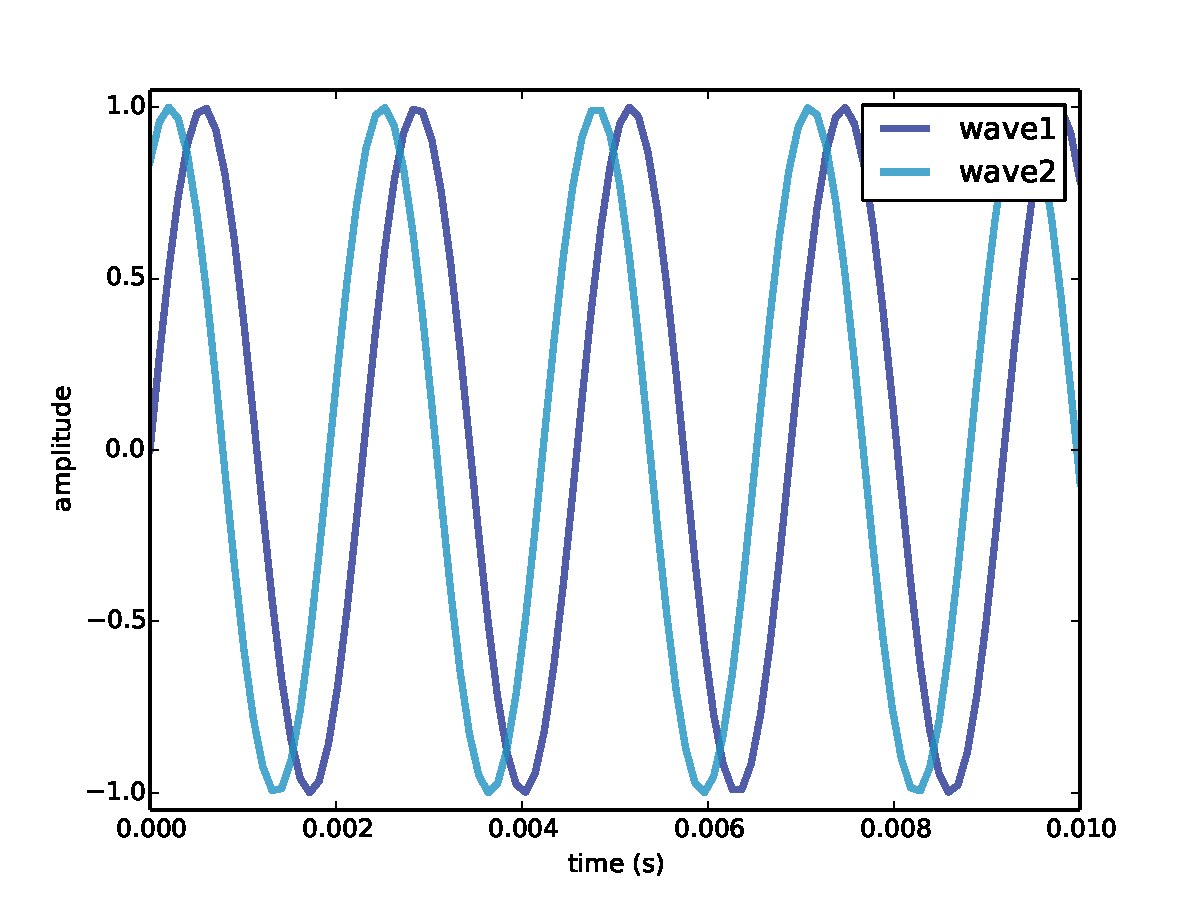
\includegraphics[height=2.5in]{figs/autocorr1.pdf}}
\caption{Two sine waves that differ by a phase offset of 1 radian;
their coefficient of correlation is 0.54.}
\label{fig.autocorr1}
\end{figure}

I'll present an example with only two variables.  First, I define
a function that constructs sine waves with different phase offsets:

\begin{verbatim}
def make_wave(offset):
    signal = thinkdsp.SinSignal(freq=440, offset=offset)
    wave = signal.make_wave(duration=0.5, framerate=10000)
    return wave
\end{verbatim}

Next I instantiate two waves with different offsets:

\begin{verbatim}
    wave1 = make_wave(offset=0)
    wave2 = make_wave(offset=1)
\end{verbatim}

Figure~\ref{fig.autocorr1} shows what the first few periods of these
waves look like.  When one wave is high, the other is usually high, so we
expect them to be correlated.

\begin{verbatim}
>>> corr_matrix = numpy.corrcoef(wave1.ys, wave2.ys, ddof=0)
[[ 1.    0.54]
 [ 0.54  1.  ]]
\end{verbatim}

The option {\tt ddof=0} indicates that {\tt corrcoef} should
divide by $N$ rather than the default, $N-1$.

The result is a correlation matrix:
the first element is the correlation of {\tt wave1}
with itself, which is always 1.  Similarly, the last element
is the correlation of {\tt wave2} with itself.

\begin{figure}
% autocorr.py
\centerline{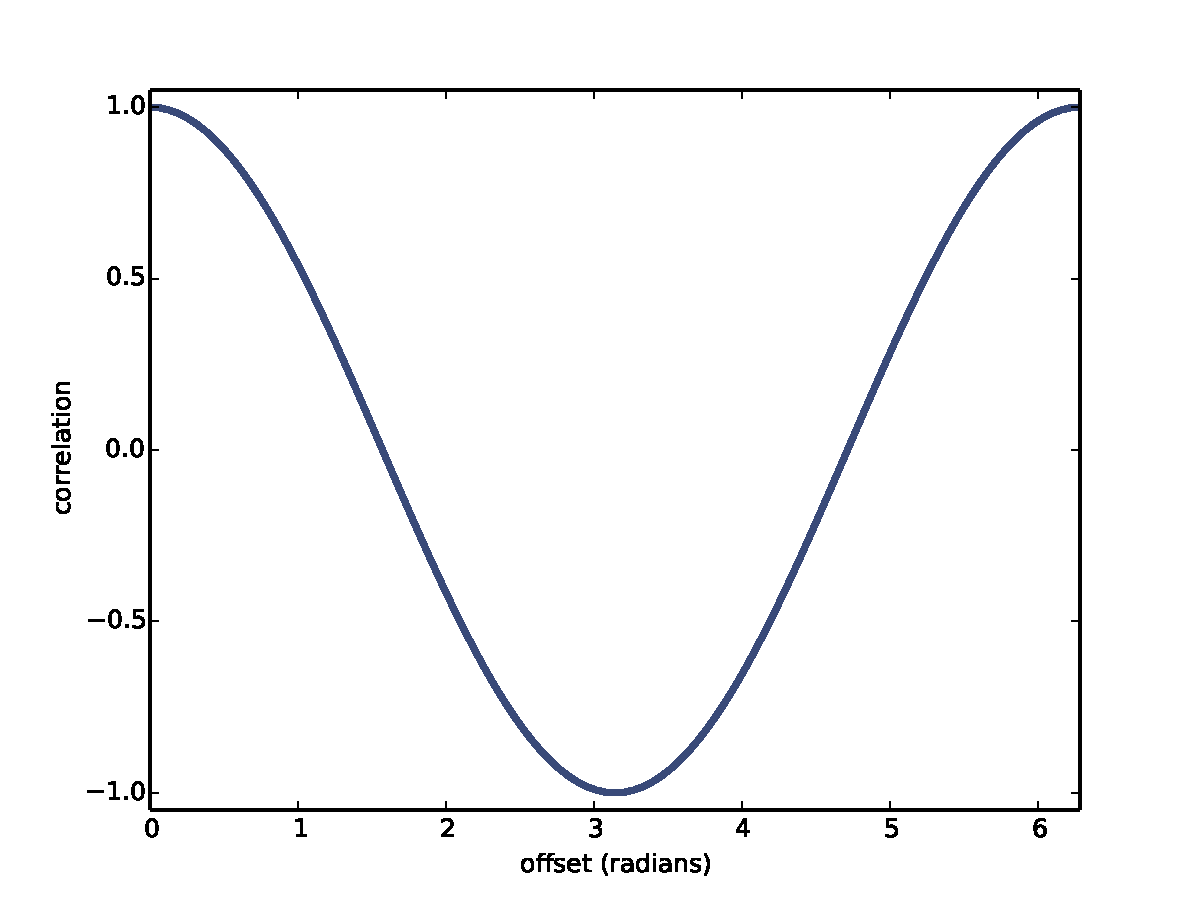
\includegraphics[height=2.5in]{figs/autocorr2.pdf}}
\caption{The correlation of two sine waves as a function of the
phase offset between them.  The result is a cosine.}
\label{fig.autocorr2}
\end{figure}

The off-diagonal elements contain the value we're interested in,
the correlation of {\tt wave1} and {\tt wave2}.  The value 0.54
indicates that the strength of the correlation is moderate.

As the phase offset increases, this correlation decreases until
the waves are 180 degrees out of phase, which yields correlation
-1.  Then it increases until the offset differs by 360 degrees.
At that point we have come full circle and the correlation is 1.

Figure~\ref{fig.autocorr2} shows the relationship between correlation and
phase offset for a sine wave.  The shape of that curve should look
familiar; it is a cosine.  This result makes sense if you remember
that the dot product of unit vectors is $\cos \theta$, where $\theta$
is the angle between the vectors.

{\tt thinkdsp} also provides a simple interface for computing the
correlation between waves:

\begin{verbatim}
>>> wave1.corr(wave2)
0.54
\end{verbatim}


\section{Serial correlation}

Signals often represent measurements of quantities that vary in
time.  For example, the sound signals we've worked with represent
measurements of voltage (or current), which represent the changes
in air pressure we perceive as sound.

Measurements like this almost always have serial correlation, which
is the correlation between each element and the next (or the previous).
To compute serial correlation, we can shift a signal and then compute
the correlation of the shifted version with the original.

\begin{verbatim}
def corrcoef(xs, ys):
    return numpy.corrcoef(xs, ys, ddof=0)[0, 1]

def serial_corr(wave, lag=1):
    n = len(wave)
    y1 = wave.ys[lag:]
    y2 = wave.ys[:n-lag]
    corr = numpy.corrcoef(y1, y2)[0, 1]
    return corr
\end{verbatim}

{\tt corrcoef} is a convenience function that simplifies
the interface to {\tt numpy.corrcoef}.

\verb"serial_corr" takes a Wave object and
{\tt lag}, which is the integer number of places to shift the waves.

We can test this function with the noise signals from the previous
chapter.  We expect UU noise to be uncorrelated, based on the
way it's generated (not to mention the name):

\begin{verbatim}
signal = thinkdsp.UncorrelatedGaussianNoise()
wave = signal.make_wave(duration=0.5, framerate=11025)
serial_corr(wave)
\end{verbatim}

When I ran this example, I got 0.006, which indicates a very
small serial correlation.  You might get a different value when you run
it, but it should be comparably small.

In a Brownian noise signal, each value is the sum of the previous
value and a random ``step,'' so we expect a strong serial
correlation:

\begin{verbatim}
signal = thinkdsp.BrownianNoise()
wave = signal.make_wave(duration=0.5, framerate=11025)
serial_corr(wave)
\end{verbatim}

Sure enough, the result I got is greater than 0.999.

\begin{figure}
% autocorr.py
\centerline{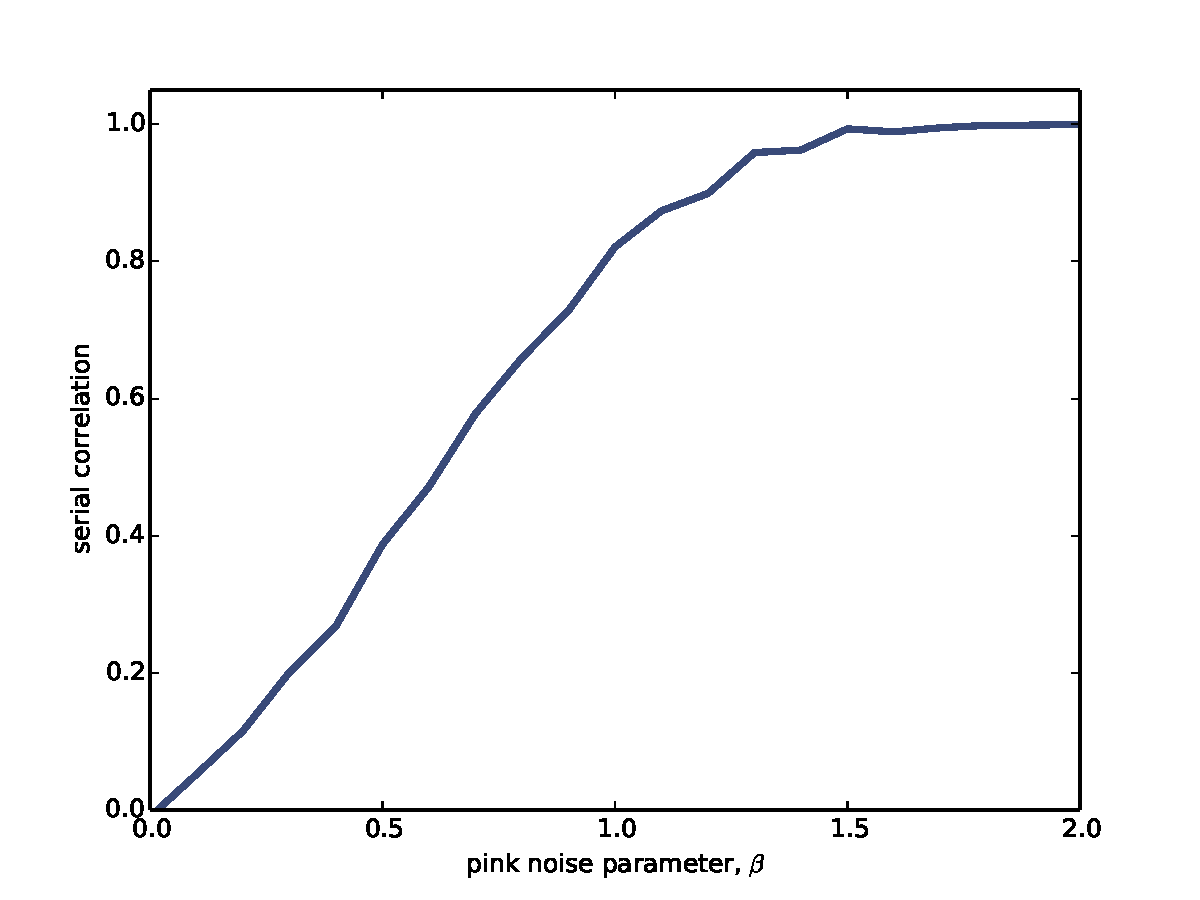
\includegraphics[height=2.5in]{figs/autocorr3.pdf}}
\caption{Serial correlation for pink noise with a range of
parameters.}
\label{fig.autocorr3}
\end{figure}

Since pink noise is in some sense between Brownian noise and UU noise,
we might expect an intermediate correlation:

\begin{verbatim}
signal = thinkdsp.PinkNoise(beta=1)
wave = signal.make_wave(duration=0.5, framerate=11025)
serial_corr(wave)
\end{verbatim}

With parameter $\beta=1$, I got a serial correlation of 0.851.
As we vary the parameter from $\beta=0$, which is uncorrelated
noise, to $\beta=2$, which is Brownian, serial correlation
ranges from 0 to almost 1, as shown in Figure~\ref{fig.autocorr3}.


\section{Autocorrelation}

In the previous section we computed the correlation between each
value and the next, so we shifted the elements of the array by 1.
But if you noticed the {\tt lag} parameter in \verb"serial_corr",
you realize we can compute serial correlations with
different lags.

\begin{figure}
% autocorr.py
\centerline{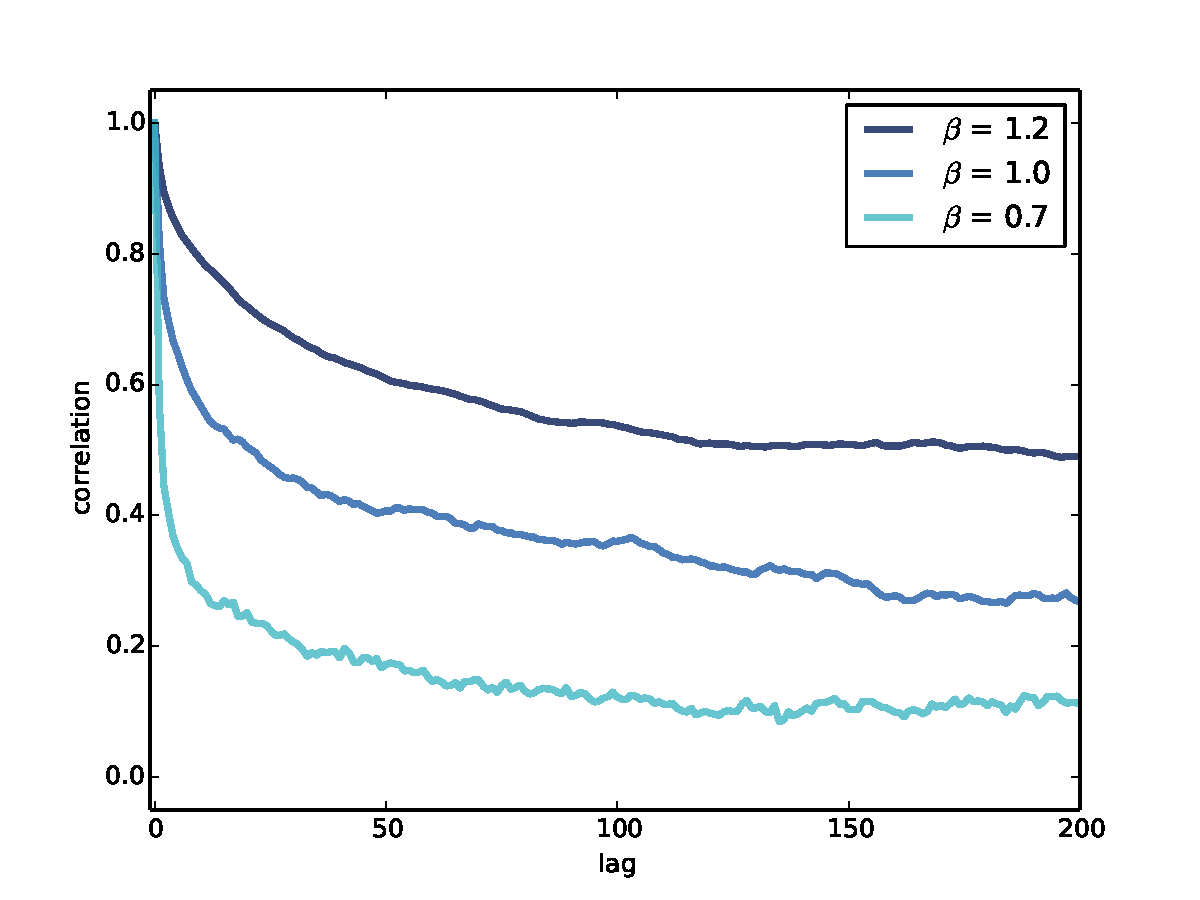
\includegraphics[height=2.5in]{figs/autocorr4.pdf}}
\caption{Autocorrelation functions for pink noise with a range
of parameters.}
\label{fig.autocorr4}
\end{figure}

In fact, we can think of \verb"serial_corr" as a function that
maps from each value of lag to the corresponding correlation, and we
can plot that function by looping through values of {\tt lag}:

\begin{verbatim}
def autocorr(wave):
    lags = range(len(wave.ys)//2)
    corrs = [serial_corr(wave, lag) for lag in lags]
    return lags, corrs
\end{verbatim}

{\tt autocorr} takes a Wave object and returns the autocorrelation
function as a pair of sequences: {\tt lags} is a sequence of
integers from 0 to half the length of the wave; {\tt corrs}
is the sequence of serial correlations for each lag.

Figure~\ref{fig.autocorr4} shows autocorrelation functions for pink
noise with three values of $\beta$.  For low values of $\beta$, the
signal is less correlated, and the autocorrelation function drops off
toward zero relatively quickly.  For larger values, serial correlation
is stronger and drops off more slowly.  Even for long lags, serial
correlation is quite strong; this phenomenon is called {\bf long-range
  dependence}, because it indicates that each value in the signal
depends on many preceding values.

If you plot these autocorrelation functions on a log-x scale, they
are approximately straight lines, which indicates that they are
decreasing exponentially.  An exponential autocorrelation function
is one of the identifying characteristics of pink noise.


\section{Autocorrelation of periodic signals}

The autocorrelation of pink noise has interesting mathematical
properties, but limited applications.  The autocorrelation of
periodic signals is more useful.

\begin{figure}
% autocorr.py
\centerline{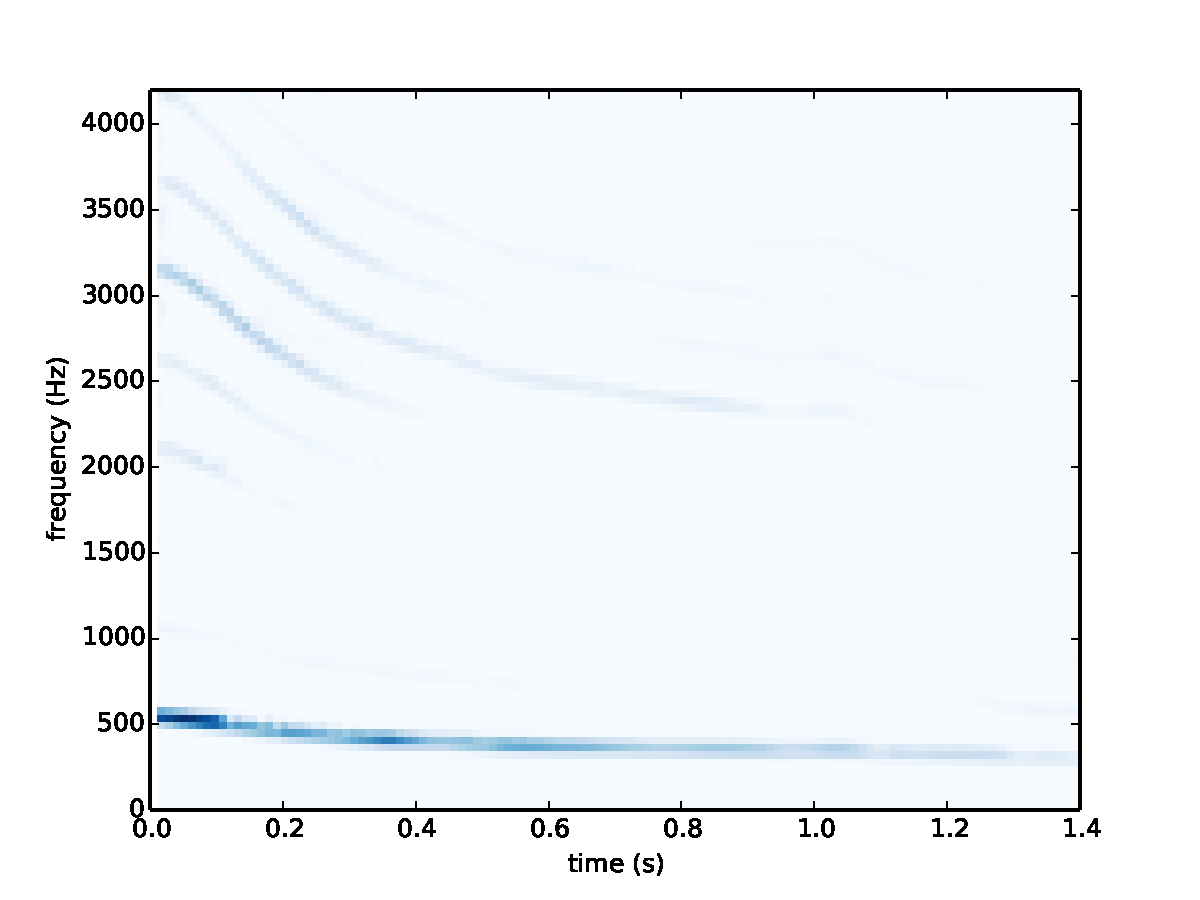
\includegraphics[height=2.5in]{figs/autocorr5.pdf}}
\caption{Spectrogram of a vocal chirp.}
\label{fig.autocorr5}
\end{figure}

As an example, I downloaded from \url{freesound.org} a recording of
someone singing a chirp; the repository for this book includes the
file: \url{28042__bcjordan__voicedownbew.wav}.  And you can use the
IPython notebook for this chapter, {\tt chap05.ipynb}, to play it.

Figure~\ref{fig.autocorr5} shows the spectrogram of this wave.
The fundamental frequency and some of the harmonics show up clearly.
The chirp starts near 500 Hz and drops down to about 300 Hz, roughly
from C5 to E4.

\begin{figure}
% autocorr.py
\centerline{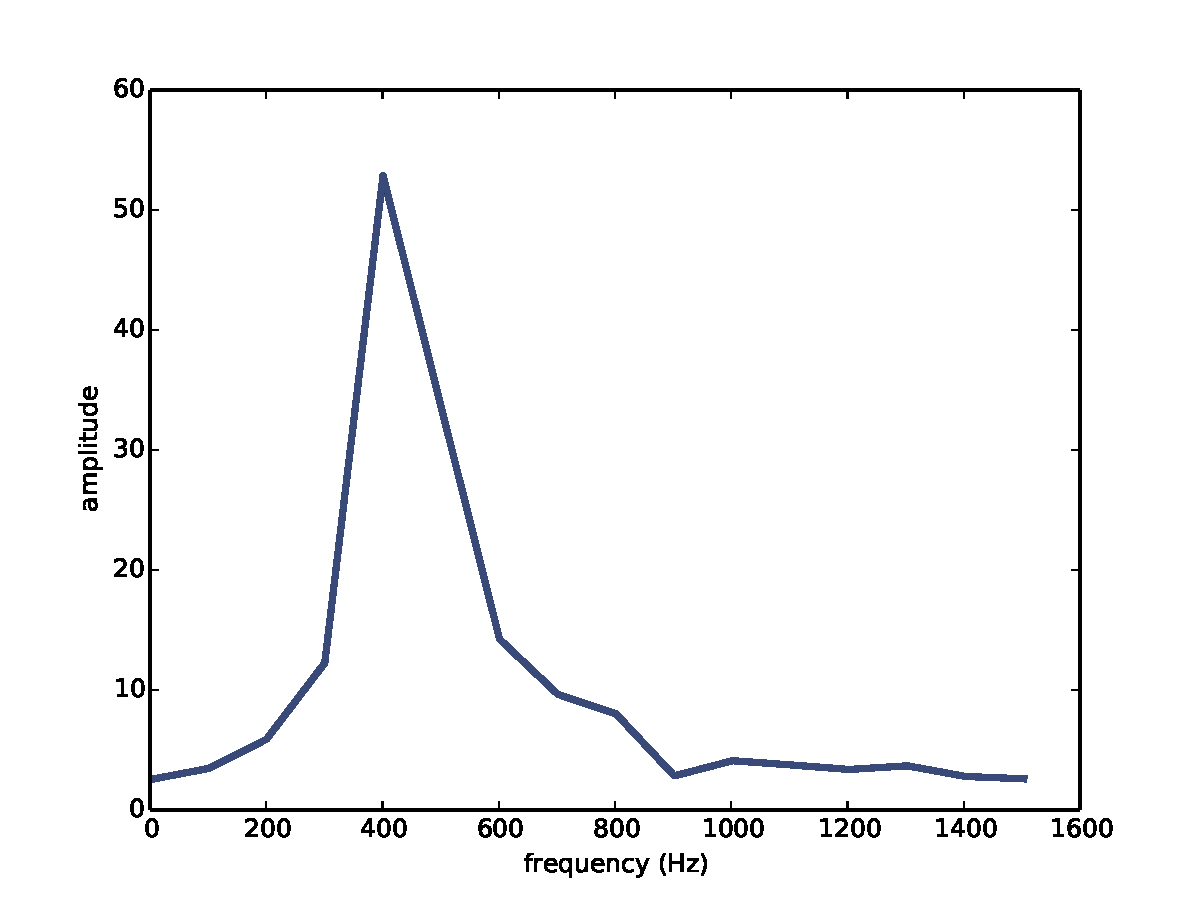
\includegraphics[height=2.5in]{figs/autocorr6.pdf}}
\caption{}
\label{fig.autocorr6}
\end{figure}

To estimate pitch at a particular point in time, we can take
a short segment from the wave and plot its spectrum:

\begin{verbatim}
    duration = 0.01
    segment = wave.segment(start=0.2, duration=duration)
    spectrum = segment.make_spectrum()
    spectrum.plot(high=15)
\end{verbatim}

This segment starts at 0.2 seconds and lasts 0.01 seconds.
Figure~\ref{fig.autocorr6} shows its spectrum.  There is a clear peak near
400 Hz, but it is hard to identify the pitch precisely.  The length of
the segment is 441 samples at a framerate of 44100 Hz, so the
frequency resolution is 100 Hz (see Section~\ref{gabor}).

If we take a longer segment, we get better frequency resolution, but
since the pitch is changing over time, we would see ``motion blur'';
that is, the peak would be spread between the start and end pitch
of the segment.

We can estimate pitch more precisely using autocorrelation.
If a signal is periodic, we expect the autocorrelation to spike
when the lag equals the period.

\begin{figure}
% autocorr.py
\centerline{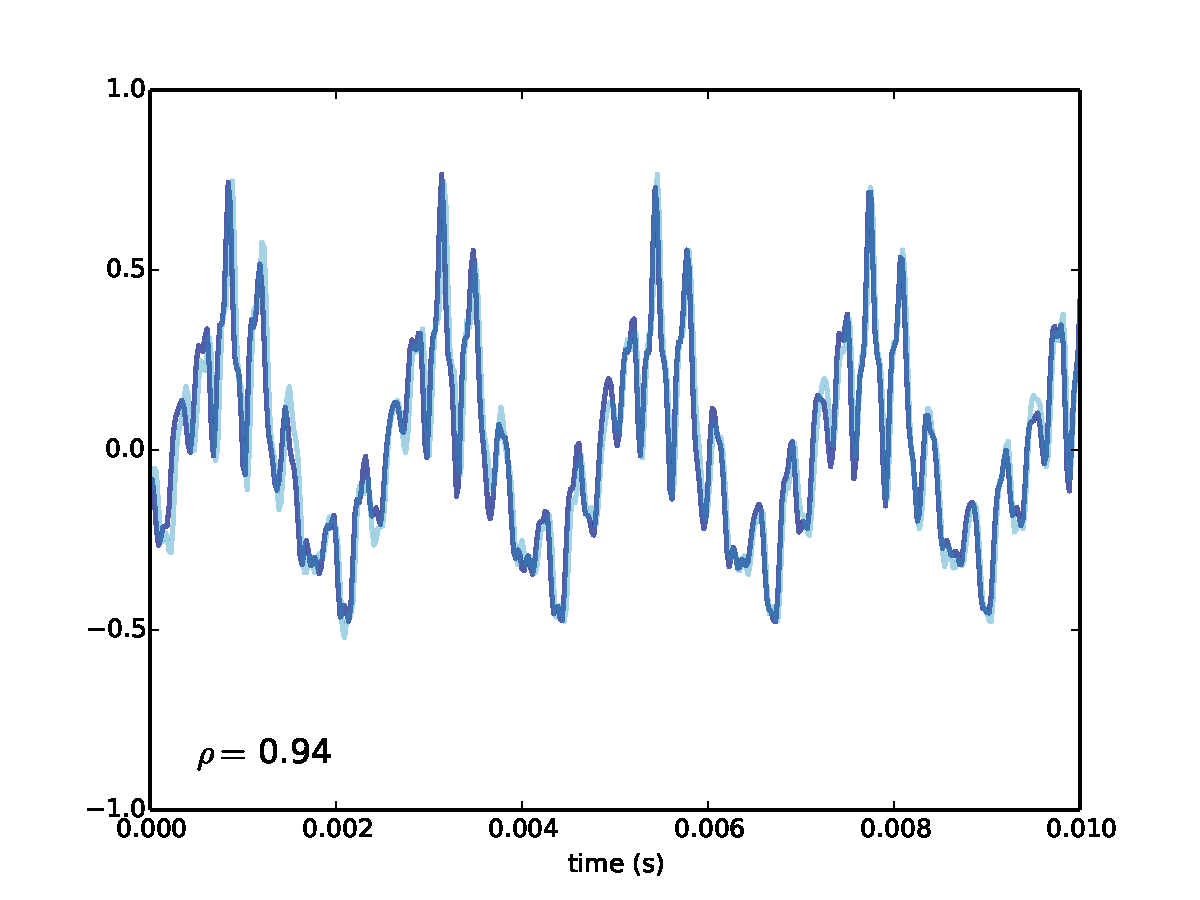
\includegraphics[height=2.5in]{figs/autocorr7.pdf}}
\caption{Two segments from a chirp, one starting 0.0023 seconds
after the other.}
\label{fig.autocorr7}
\end{figure}

To show why that works, I'll plot two segments from the same
recording.

\begin{verbatim}
def plot_shifted(wave, shift=0.0023, start=0.2):
    thinkplot.preplot(2)
    segment1 = wave.segment(start=start, duration=0.01)
    segment1.plot(linewidth=2, alpha=0.8)

    segment2 = wave.segment(start=start-shift, duration=0.01)
    segment2.plot(linewidth=2, alpha=0.4)

    thinkplot.config(xlabel='time (s)', ylim=[-1, 1])
\end{verbatim} 

One segment starts at 0.2 seconds; the other starts 0.0023 seconds
later.  Figure~\ref{fig.autocorr7} shows the result.  The segments
are similar, and their correlation is 0.94.  This result suggests
that the period is near 0.0023 seconds, which corresponds to a frequency
of 435 Hz.

\begin{figure}
% autocorr.py
\centerline{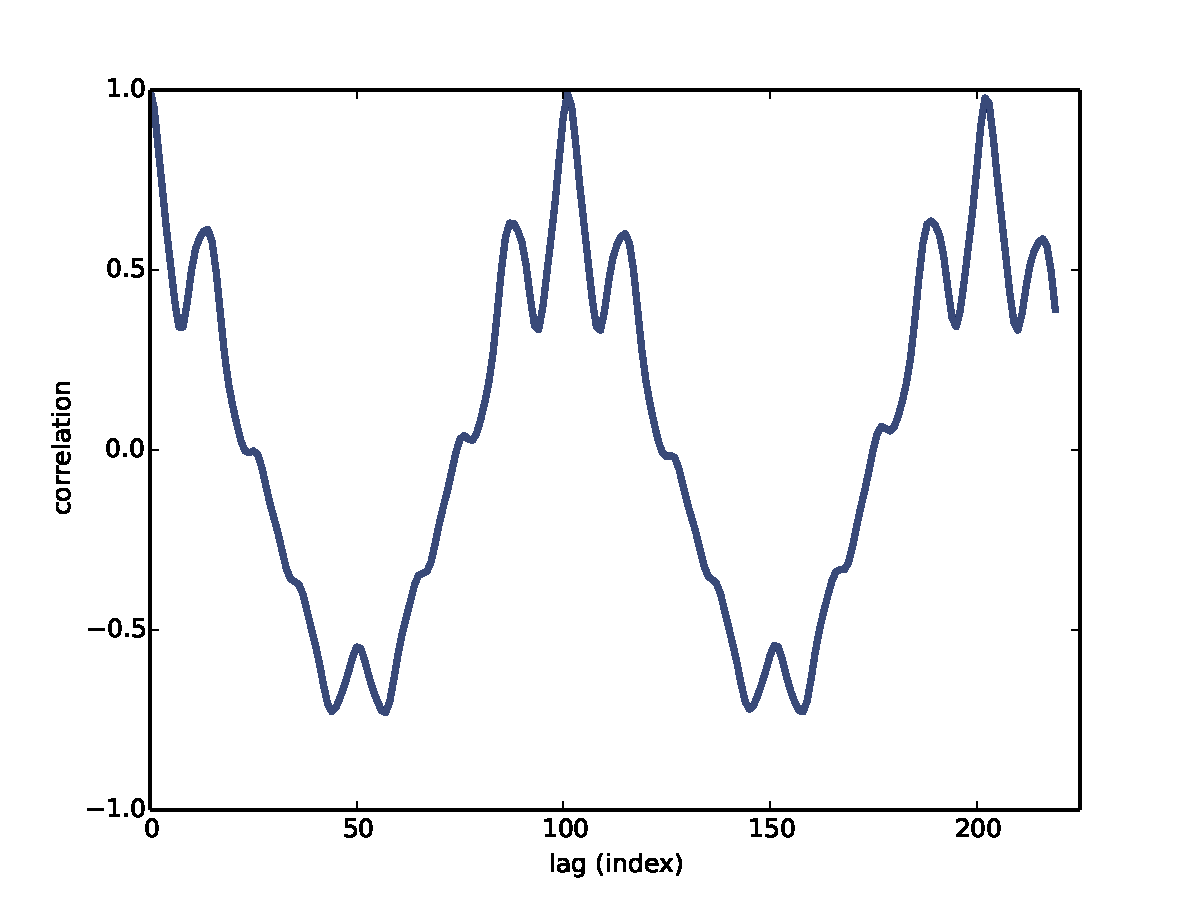
\includegraphics[height=2.5in]{figs/autocorr8.pdf}}
\caption{Autocorrelation function for a segment from a chirp.}
\label{fig.autocorr8}
\end{figure}

In this example, I estimated the period by trial and error.  To automate
this process, we can use the autocorrelation function.

\begin{verbatim}
    lags, corrs = autocorr(segment)
    thinkplot.plot(lags, corrs)
\end{verbatim}

Figure~\ref{fig.autocorr8} shows the autocorrelation function for
the segment starting at $t=0.2$ seconds.  The first peak occurs at
{\tt lag=101}.  Then we can compute the frequency that corresponds
to that period:

\begin{verbatim}
    period = lag / segment.framerate
    frequency = 1 / period
\end{verbatim}

The estimated fundamental frequency is 437 Hz.  To evaluate the
precision of the estimate, we can run the same computation with
lags 100 and 102, which correspond to frequencies 432 and 441 Hz.
So the frequency precision using autocorrelation is less than 10 Hz,
compared with 100 Hz using the spectrum.


\section{Using NumPy}
\label{correlate}

\begin{figure}
% autocorr.py
\centerline{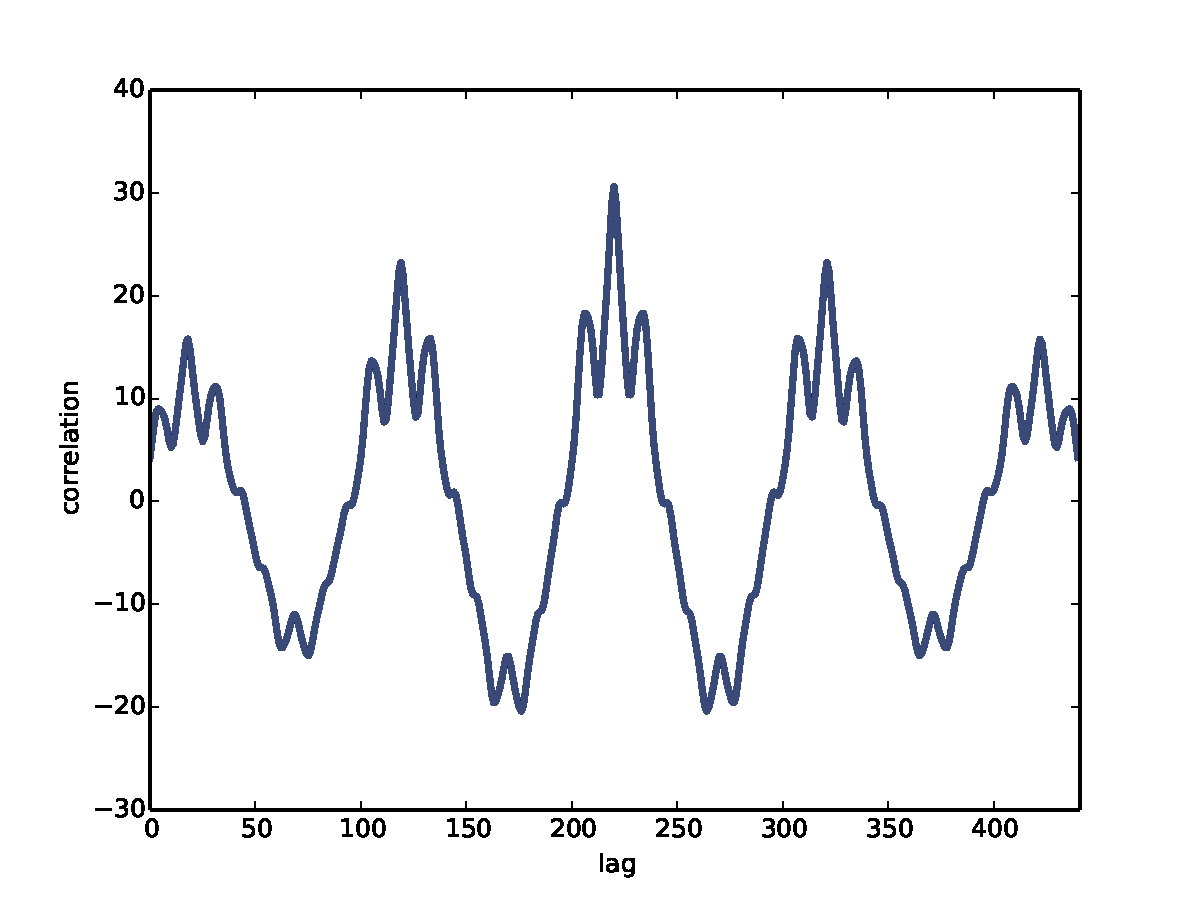
\includegraphics[height=2.5in]{figs/autocorr9.pdf}}
\caption{Autocorrelation function computed with {\tt numpy.correlate}.}
\label{fig.autocorr9}
\end{figure}

NumPy provides a function, {\tt correlate}, that computes
the correlation of two functions or the autocorrelation of one
function.  We can use it to compute the autocorrelation of
the segment from the previous section:

\begin{verbatim}
corrs2 = numpy.correlate(segment.ys, segment.ys, mode='same')
\end{verbatim}

The option {\tt mode} tells {\tt correlate} what range
of {\tt lag} it should use.  With the value {\tt 'same'}, the
range is from $-N/2$ to $N/2$, where $N$ is the length of the
wave array.

Figure~\ref{fig.autocorr9} shows the result.  It is symmetric because
the two signals are identical, so a negative lag on one has the same
effect as a positive lag on the other.  To compare with the results
from {\tt autocorr}, we can select the second half:

\begin{verbatim}
    N = len(corrs2)
    half = corrs2[N//2:]
\end{verbatim}

If you compare Figure~\ref{fig.autocorr9} to Figure~\ref{fig.autocorr8},
you'll notice that the correlations computed by {\tt numpy.correlate}
get smaller as the lags increase.  As the lag get bigger, the amount of
overlap between the two signals gets smaller, so the magnitude of
the correlations decreases.

We can correct that by dividing through by the lengths:

\begin{verbatim}
    lengths = range(N, N//2, -1)
    half /= lengths
\end{verbatim}

Finally, we can normalize the results so the correlation with
{\tt lag=0} is 1.

\begin{verbatim}
    half /= half[0]
\end{verbatim}

With these adjustments, the results computed by {\tt autocorr} and
{\tt numpy.correlate} are nearly the same, but they still differ by
1-2\%.  The reason not important, but if you are curious: {\tt autocorr}
normalizes the correlations independently for each lag; for
{\tt numpy.correlate}, we normalized them all at the end.

More importantly, now you know what autocorrelation is, how to
use it to estimate the fundamental period of a signal, and two
ways to compute it.


\section{Exercises}

\begin{exercise}
If you did the exercises in the previous chapter, you downloaded
the historical price of BitCoins and estimated the power spectrum
of the price changes.  Using the same data, compute the autocorrelation
of BitCoin prices.  Does the autocorrelation function decay
exponentially?  Is there evidence of periodic behavior?
\end{exercise}

\begin{exercise}
% TODO: finish this exercise
Estimate the pitch of a segment from the saxophone recording.
\end{exercise}



\chapter{Discrete cosine transform}
\label{dct}

The code for this chapter is available from
\url{http://think-dsp.com/dct.py}.

The topic of this chapter is the {\bf Discrete Cosine
  Transform} (DCT), which is used in MP3 and related formats for
compressing music, JPEG and similar formats for images, and the MPEG
family of formats for video.

DCT is similar in many ways to the discrete Fourier transform (DFT),
which we have been using for spectral analysis.
Once we learn how DCT works, it will be easier to explain DFT.

Here are the steps we'll follow to get there:

\begin{enumerate}

\item We'll start with the synthesis problem: given a set of frequency
  components and their amplitudes, how can we construct a waveform?

\item Next we'll rewrite the synthesis problem using NumPy arrays.
  This move is good for performance, and also provides insight
  for the next step.

\item We'll look at the analysis problem: given a signal and a
  set of frequencies, how can we find the amplitude of each frequency
  component?  We'll start with a solution that is conceptually simple
  but slow.

\item Finally, we'll use some principles from linear algebra to find a
  more efficient algorithm.  If you already know linear algebra,
  that's great, but I will explain what you need as we go.

\end{enumerate}

Let's get started.


\section{Synthesis}
\label{synth1}

Suppose I give you a list of amplitudes and a list of frequencies,
and ask you to construct a signal that is the sum of these frequency
components.  Using objects in the {\tt thinkdsp} module, there is
a simple way to perform this operation, which is called {\bf synthesis}:

\begin{verbatim}
def synthesize1(amps, freqs, ts):
    components = [thinkdsp.CosSignal(freq, amp)
                  for amp, freq in zip(amps, freqs)]
    signal = thinkdsp.SumSignal(*components)

    ys = signal.evaluate(ts)
    return ys
\end{verbatim}

{\tt amps} is a list of amplitudes, {\tt freqs} is the list
of frequencies, and {\tt ts} is the sequence
of times where the signal should be evaluated.

{\tt components} is a list of {\tt CosSignal} objects, one for
each amplitude-frequency pair.  {\tt SumSignal} represents the
sum of these frequency components.

Finally, {\tt evaluate} computes the value of the signal at each
time in {\tt ts}.

We can test this function like this:

\begin{verbatim}
    amps = numpy.array([0.6, 0.25, 0.1, 0.05])
    freqs = [100, 200, 300, 400]
    framerate = 11025

    ts = numpy.linspace(0, 1, framerate)
    ys = synthesize1(amps, freqs, ts)
    wave = thinkdsp.Wave(ys, framerate)
    wave.play()
\end{verbatim}

This example makes a signal that contains a fundamental frequency at
100 Hz and three harmonics (100 Hz is a sharp G2).  It renders the
signal for one second at 11,025 frames per second and plays the
resulting wave.

Conceptually, synthesis is pretty simple.  But in this form it doesn't
help much with {\bf analysis}, which is the inverse problem: given the
wave how do we identify the frequency components and their amplitudes?


\section{Synthesis with arrays}
\label{synthesis}

\begin{figure}
% LaTeX source for ``Think DSP: Digital Signal Processing for Programmers''
% Copyright 2013  Allen B. Downey.

% License: Creative Commons Attribution-NonCommercial 3.0 Unported License.
% http://creativecommons.org/licenses/by-nc/3.0/
%

\[ 
\begin{matrix}
& {\large \mathtt{M}} &
 \begin{bmatrix} 
0.6 \\
0.25 \\
0.1 \\
0.05 \\
\end{bmatrix}
= \mathtt{amps}
\\
\\
\begin{matrix} 
&.& \\
&.& \\
&t_n& \\
&.& \\
&.& \\
\end{matrix}
&
\begin{bmatrix} 
. & . & . & . \\
. & . & . & . \\
a & b & c & d \\
. & . & . & . \\
. & . & . & . \\
\end{bmatrix} 
&
\begin{bmatrix} 
&.& \\
&.& \\
&e& \\
&.& \\
&.& \\
\end{bmatrix} = \mathtt{ys}
\\
\\
&
\begin{matrix}
. & f_k & . & . \\
\end{matrix}
&
\\
\end{matrix}
\]


 

\caption{Synthesis with arrays.}
\label{fig.synthesis}
\end{figure}

Here's another way to write {\tt synthesize}:

\begin{verbatim}
def synthesize2(amps, freqs, ts):
    args = numpy.outer(ts, freqs)
    M = numpy.cos(PI2 * args)
    ys = numpy.dot(M, amps)
    return ys
\end{verbatim}

This function looks very different, but it does the same thing.
Let's see how it works:

\begin{enumerate}

\item {\tt numpy.outer} computes the outer product of {\tt ts} and
  {\tt freqs}.  The result is an array with one row for each element
  of {\tt ts} and one column for each element of {\tt freqs}.  Each
  element in the array is the product of a frequency and a time, $f
  t$.

\item We multiply {\tt args} by $2 \pi$ and apply {\tt cos}, so each
  element of the result is $\cos (2 \pi f t)$.  Since the {\tt ts} run
  down the columns, each column contains a cosine signal at a
  particular frequency, evaluated at a sequence of times.

\item {\tt numpy.dot} computes a dot product.  In terms of linear
  algebra, we are multiplying a matrix, {\tt M}, by a vector, {\tt
    amps}.  Figure~\ref{fig.synthesis} is a diagram of this
  multiplication.  {\tt numpy.dot} multiplies each row of {\tt M} by
  {\tt amps}, element-wise, and then adds up the products.

\end{enumerate}

Figure~\ref{fig.synthesis} shows the structure of this computation.
Each row of the matrix, {\tt M}, corresponds to a time 
from 0.0 to 1.0 s; $t_k$ is the time of the $k$th row.
Each column corresponds to a frequency from
100 to 400 Hz; $f_j$ is the frequency of the $j$th column.

I labeled the $k$th row with the letters $a$ through $d$; as an
example, the value of $a$ is $\cos [2 \pi (220) t_k]$.

The result of the dot product, {\tt ys}, is a vector with one element
for each row of {\tt M}.  The $k$th element, labeled $e$, is the sum
of products:
%
\[ e = 0.6 a + 0.25 b + 0.1 c + 0.05 d \]
%
And likewise with the other elements of {\tt ys}.  So each element
of {\tt y} is the sum of four frequency components, evaluated at
a point in time, and multiplied by the corresponding amplitudes.
And that's exactly what we wanted.  We can use the code from
the previous section to
check that the two versions of {\tt synthesize} produce the same results.

\begin{verbatim}
    amps = numpy.array([0.6, 0.25, 0.1, 0.05])
    freqs = [100, 200, 300, 400]
    framerate = 11025
    ts = numpy.linspace(0, 1, framerate)
    ys1 = synthesize1(amps, freqs, ts)
    ys2 = synthesize2(amps, freqs, ts)
    print max(abs(ys1 - ys2))
\end{verbatim}

The biggest difference between {\tt ys1} and {\tt y2} is about {\tt
  1e-13}, which is what we expect due to floating-point errors.

One note on linear algebra vocabulary: I am using ``matrix'' to refer
to a two-dimensional array, and ``vector'' for a one-dimensional array
or sequence.  To be pedantic, it would be more correct to think
of matrices and vectors as abstract mathematical concepts, and NumPy
arrays as one way (and not the only way) to represent them.

One advantage of linear algebra is that it provides concise notation
for operations on matrices and vectors.  For example, we could write
{\tt synthesize} like this:
%
\begin{eqnarray*}
M &=& \cos (2 \pi t \otimes f) \\
y &=& M a
\end{eqnarray*}
%
where $a$ is a vector of amplitudes,
$t$ is a vector of times, $f$ is a vector of frequencies, and
$\otimes$ is the symbol for the outer product of two vectors.


\section{Analysis}
\label{analysis}

Now we are ready to solve the analysis problem.  Suppose I give you
a wave and tell you that it is the sum of cosines with a given set
of frequencies.  How would you find the amplitude for each frequency
component?  In other words, given {\tt ys}, {\tt ts} and {\tt freqs},
can you recover {\tt amps}?

In terms of linear algebra, the first step is the same as for
synthesis: we compute $M = \cos (2 \pi t \otimes f)$.  Then we want
to find $a$ so that $y = M a$; in other words, we want to solve a
linear system.  NumPy provides {\tt linalg.solve}, which does
exactly that.

Here's what the code looks like:

\begin{verbatim}
def analyze1(ys, freqs, ts):
    args = numpy.outer(ts, freqs)
    M = numpy.cos(PI2 * args)
    amps = numpy.linalg.solve(M, ys)
    return amps
\end{verbatim}

The first two lines use {\tt ts} and {\tt freqs} to build the
matrix, {\tt M}.  Then {\tt numpy.linalg.solve} computes {\tt amps}.

But there's a hitch.  In general we can only solve a system of linear
equations if the matrix is square; that is, the number of equations
(rows) is the same as the number of unknowns (columns).

In this example, we have only 4 frequencies, but we evaluated the
signal at 11,025 times.  So we have many more equations than unknowns.

But in general if {\tt ys}
contains more than 4 elements, it is unlikely that we can analyze it
using only 4 frequencies.

But in this case, we know that the {\tt ys} were actually generated by
adding only 4 frequency components, so we can use any 4 values from
the wave array to recover {\tt amps}.

For simplicity, I'll use the first 4 samples from
the signal.
Using the values of {\tt ys}, {\tt freqs} and {\tt ts} from
the previous section, we can run {\tt analyze1} like this:

\begin{verbatim}
    n = len(freqs)
    amps2 = analyze1(ys[:n], freqs, ts[:n])
\end{verbatim}

And sure enough, we get

\begin{verbatim}
amps2 = [ 0.6   0.25  0.1   0.05 ]
\end{verbatim}

So this algorithm works, but it is slow.  Solving a linear
system of equations takes time proportional to $n^3$, where $n$ is
the number of columns in $M$.  We can do better.


\section{Orthogonal matrixes}

One way to solve linear systems is by inverting matrixes.  The
inverse of a matrix $M$ is written $M^{-1}$, and it has the property
that $M^{-1}M = I$.  $I$ is the identity matrix, which has
the value 1 on all diagonal elements and 0 everywhere else.

So, to solve the equation $y = Ma$, we can multiply both sides by
$M^{-1}$, which yields:
%
\[ M^{-1}y = M^{-1} M a \]
%
On the right side, we can replace $M^{-1}M$ with $I$:
%
\[ M^{-1}y = I a \]
%
If we multiply $I$ by any vector $a$, the result is $a$, so  
%
\[ M^{-1}y = a \]
%
This implies that if we can compute $M^{-1}$ efficiently, we can find
$a$ with a simple matrix multiplication (using {\tt numpy.dot}).  That
takes time proportional to $n^2$, which is better than $n^3$.

In general inverting a matrix is slow, but some special cases are
faster.  In particular, if $M$ is {\bf orthogonal}, the inverse of $M$
is just the transpose of $M$, written $M^T$.  In NumPy
transposing an array is a constant-time operation.  It
doesn't actually move the elements of the array; instead, it creates a
``view'' that changes the way the elements are accessed.

Again, a matrix is orthogonal
if its transpose is also
its inverse; that is, $M^T = M^{-1}$.  That implies that $M^TM = I$,
which means we can check whether a matrix is orthogonal by computing
$M^TM$.

So let's see what the matrix looks like in {\tt synthesize2}.  In 
the previous example, $M$ has 11,025 rows, so it might be a good idea
to work with a smaller example:

\begin{verbatim}
def test1():
    amps = numpy.array([0.6, 0.25, 0.1, 0.05])
    N = 4.0
    time_unit = 0.001
    ts = numpy.arange(N) / N * time_unit
    max_freq = N / time_unit / 2
    freqs = numpy.arange(N) / N * max_freq
    ys = synthesize2(amps, freqs, ts)
\end{verbatim}

{\tt amps} is the same vector of amplitudes we saw before.
Since we have 4 frequency components, we'll sample the signal
at 4 points in time.  That way, $M$ is square.

{\tt ts} is a vector of equally spaced sample times in the range from
0 to 1 time unit.  I chose the time unit to be 1 millisecond, but it
is an arbitrary choice, and we will see in a minute that it drops out
of the computation anyway.

Since the frame rate is $N$ samples per time unit, the Nyquist
frequency is \verb"N / time_unit / 2", which is 2000 Hz in this
example.  So {\tt freqs} is a vector of equally spaced frequencies
between 0 and 2000 Hz.

With these values of {\tt ts} and {\tt freqs}, the matrix, $M$, is:

\begin{verbatim}
[[ 1.     1.     1.     1.   ]
 [ 1.     0.707  0.    -0.707]
 [ 1.     0.    -1.    -0.   ]
 [ 1.    -0.707 -0.     0.707]]
\end{verbatim}

You might recognize 0.707 as an approximation of $\sqrt{2}/2$,
which is $\cos \pi/4$.  You also might notice that this matrix
is {\bf symmetric}, which means that the element at $(j, k)$ always
equals the element at $(k, j)$.  This implies that $M$ is its own
transpose; that is $M^T = M$.

But sadly, $M$ is not orthogonal.  If we compute $M^TM$, we get:

\begin{verbatim}
[[ 4.  1. -0.  1.]
 [ 1.  2.  1. -0.]
 [-0.  1.  2.  1.]
 [ 1. -0.  1.  2.]]
\end{verbatim}

And that's not the identity matrix.


\section{DCT-IV}

But if we choose {\tt ts} and {\tt freqs} carefully,
we can make $M$ orthogonal.  There are several ways to do it, which
is why there are several versions of the discrete cosine transform (DCT).

One simple option is to shift {\tt ts} and {\tt freqs} by a half unit.
This version is called DCT-IV, where ``IV'' is a roman numeral
indicating that this is the fourth of eight versions of the DCT.

Here's an updated version of {\tt test1}:

\begin{verbatim}
def test2():
    amps = numpy.array([0.6, 0.25, 0.1, 0.05])
    N = 4.0
    ts = (0.5 + numpy.arange(N)) / N
    freqs = (0.5 + numpy.arange(N)) / 2
    ys = synthesize2(amps, freqs, ts)
\end{verbatim}

If you compare this to the previous version, you'll notice
two changes.  First, I added 0.5 to {\tt ts} and {\tt freqs}.
Second, I cancelled out \verb"time_units", which simplifies
the expression for {\tt freqs}.

With these values, $M$ is

\begin{verbatim}
[[ 0.981  0.831  0.556  0.195]
 [ 0.831 -0.195 -0.981 -0.556]
 [ 0.556 -0.981  0.195  0.831]
 [ 0.195 -0.556  0.831 -0.981]]
\end{verbatim}

And $M^TM$ is

\begin{verbatim}
[[ 2.  0.  0.  0.]
 [ 0.  2. -0.  0.]
 [ 0. -0.  2. -0.]
 [ 0.  0. -0.  2.]]
\end{verbatim}

Some of the off-diagonal elements are displayed as -0, which means
that the floating-point representation is a small negative number.  So
this matrix is very close to $2I$, which means $M$ is almost
orthogonal; it's just off by a factor of 2.  And for our purposes,
that's good enough.

Because $M$ is symmetric and (almost) orthogonal, the inverse of $M$
is just $M/2$.  Now we can write a more efficient version of {\tt
  analyze}:

\begin{verbatim}
def analyze2(ys, freqs, ts):
    args = numpy.outer(ts, freqs)
    M = numpy.cos(PI2 * args)
    amps = numpy.dot(M, ys) / 2
    return amps
\end{verbatim}

Instead of using {\tt numpy.linalg.solve}, we just multiply
by $M/2$.

Putting it all together, we can write an implementation of
DCT-IV:

\begin{verbatim}
def dct_iv(ys):
    N = len(ys)
    ts = (0.5 + numpy.arange(N)) / N
    freqs = (0.5 + numpy.arange(N)) / 2
    args = numpy.outer(ts, freqs)
    M = numpy.cos(PI2 * args)
    amps = numpy.dot(M, ys) / 2
    return amps
\end{verbatim}

Again, {\tt ys} is the wave array.  We don't have to pass
{\tt ts} and {\tt freqs} as parameters; \verb"dct_iv" can
figure them out based on {\tt N}, the length of {\tt ys}.

We can test \verb"dct_iv" like this

\begin{verbatim}
    amps = numpy.array([0.6, 0.25, 0.1, 0.05])
    N = 4.0
    ts = (0.5 + numpy.arange(N)) / N
    freqs = (0.5 + numpy.arange(N)) / 2
    ys = synthesize2(amps, freqs, ts)

    amps2 = dct_iv(ys)
    print max(abs(amps - amps2))
\end{verbatim}

Starting with {\tt amps}, we synthesize a wave array, then use
\verb"dct_iv" to see if we can recover the amplitudes.  The biggest
difference between {\tt amps} and {\tt amps2} is about {\tt 1e-16},
which is what we expect with 64-bit floating point arithmetic.


\section{Inverse DCT}

Finally, notice that {\tt analyze2} and {\tt synthesize2} are almost
identical.  The only difference is that {\tt analyze2} divides the
result by 2.  We can use this insight to compute the inverse DCT:

\begin{verbatim}
def inverse_dct_iv(amps):
    return dct_iv(amps) * 2
\end{verbatim}

\verb"inverse_dct_iv" takes the vector of amplitudes and returns
the wave array, {\tt ys}.  We can confirm that it works by starting
with {\tt amps}, applying \verb"inverse_dct_iv" and \verb"dct_iv",
and testing that we get back what we started with.

\begin{verbatim}
    amps = [0.6, 0.25, 0.1, 0.05]
    ys = inverse_dct_iv(amps)
    amps2 = dct_iv(ys)
    print max(abs(amps - amps2))
\end{verbatim}

Again, the biggest difference is about {\tt 1e-16}.


\section{Summary}

This chapter explores the relationship between the synthesis problem
and the analysis problem.  By writing the synthesis problem in the
form of matrix operations, we derive an efficient algorithm for computing
the DCT.

This algorithm is based on a matrix, $M$, that is orthogonal and
symmetric, so it has the unusual property that the inverse of $M$ is
$M$ (within a factor of two, anyway).  As a result, the function we
wrote to compute DCT-IV also computes the inverse DCT.

For the analysis problem, we started with a solution that
takes time proportional to $n^3$ and improved it to take time
proportional to $n^2$.  It turns out that there is another optimization
that gets the run time down to $n \log n$.  We'll see how that works
in Chapter~\ref{???}.



\section{Exercises}

\begin{exercise}
Test the algorithmic complexity of {\tt analyze1}, {\tt analyze2}
and {\tt scipy.fftpack.dct}.
\end{exercise}

\begin{exercise}
One of the major applications of the DCT is compression for both
sound and images.  For example, MP3 uses a compression algorithm
based on the DCT.  In it's simplest form, DCT-based compression
works like this:

\begin{enumerate}

\item Break a long signal into segments.

\item Compute the DCT of each segment.

\item Identify frequency components with amplitudes so low they are
  inaudible, and remove them.  Store only the frequencies and
  amplitudes that remain.

\item To play back the signal, load the frequencies and amplitudes
  for each segment and apply the inverse DCT.

\end{enumerate}

Implement a version of this algorithm and apply it to a recording
of music or speech.  How many components can you eliminate before
the difference is perceptible?

\end{exercise}



\chapter{Discrete Fourier Transform}
\label{dft}

We've been using the discrete Fourier transform (DFT) since
Chapter~\ref{sounds}, but I haven't explained how it works.  Now is
the time.

If you understand the discrete cosine transform (DCT), you will
understand the DFT.  The only difference is that instead of using the
cosine function, we'll use the complex exponential function.  I'll
start by explaining complex exponentials, then I'll follow the
same progression you saw in Chapter~\ref{dct}:

\begin{enumerate}

\item I'll start with the synthesis
  problem: given a set of frequency components and their amplitudes,
  how can we construct a signal?  The synthesis problem is 
  equivalent to the inverse DFT.

\item Then I'll rewrite the synthesis problem in the form of matrix
  multiplication using NumPy arrays.

\item Next we'll solve the analysis problem, which is equivalent to
  the DFT: given a signal, how to we find the amplitude and phase
  offset of its frequency components?

\item Finally, we'll use linear algebra to find a more efficient way
  to compute the DFT.

\end{enumerate}

The code for this chapter is in {\tt dft.py}, which is in the
repository for this book (see Section~\ref{code}).


\section{Complex exponentials}

One of the more interesting moves in mathematics is the generalization
of an operation from one type to another.  For example, factorial
is a function that operates on integers; the natural definition for
factorial of $n$ is the product of all integers from 1 to $n$.

If you are of a certain inclination, you might wonder how to compute
the factorial of a non-integer like 3.5.  Since the natural definition
doesn't apply, you might look for other ways to compute the factorial
function, ways that would work with non-integers.

In 1730, Leonhard Euler found one, a generalization of the factorial
function that we know as the gamma function (see
\url{http://en.wikipedia.org/wiki/Gamma_function}).

Euler also found one of the most useful generalizations in applied
mathematics, the complex exponential function.

The natural definition of exponentiation is repeated multiplication.
For example, $\phi^3 = \phi \cdot \phi \cdot \phi$.  But this
definition doesn't apply to non-integers, including complex numbers.

But exponentiation can also be expressed as a power series:
%
\[ e^\phi = 1 + \phi + \phi^2/2! + \phi^3/3! + ... \]
%
This definition works with imaginary numbers and, by a simple
extension, with complex numbers.  It turns out that:
%
\[ e^{i\phi} = \cos \phi + i \sin \phi \]
%
You can see the derivation at
\url{http://en.wikipedia.org/wiki/Euler's_formula}.  This formula
implies that $e^{i\phi}$ is a complex number with magnitude 1; if you
think of it as a point in the complex plane, it is always on the unit
circle.  And if you think of it as a vector, the angle in radians
between the vector and the positive x-axis is the argument, $\phi$.

In the case where the argument is a complex number, we have:
%
\[ e^{a + i\phi} = e^a e^{i\phi} = A e^{i\phi} \]
%
where $A$ is a real number that indicates amplitude and
$e^{i\phi}$ is a complex number with magnitude 1.

NumPy provides a version of {\tt exp} that works with
complex numbers:

\begin{verbatim}
>>> i = complex(0, 1)
>>> phi = 1.5
>>> z = numpy.exp(i * phi)
>>> z
(0.0707+0.997j)
\end{verbatim}

{\tt complex} is a built-in function that takes the real and
imaginary parts of a complex number and returns a Python
complex object.

When the argument to {\tt numpy.exp} is imaginary or complex, the
result is a complex number; specifically, a {\tt numpy.complex128},
which is represented by two 64-bit floating-point numbers.  The result
is {\tt 0.0707+0.997j}.  Note that Python uses {\tt j} to represent
the imaginary unit, rather than {\tt i}.

Complex numbers have attributes {\tt real} and {\tt imag}:

\begin{verbatim}
>>> z.real
0.0707
>>> z.imag
0.997
\end{verbatim}

To get the magnitude, you can use the built-in function {\tt abs}
or {\tt numpy.absolute}:

\begin{verbatim}
>>> abs(z)
1.0
>>> numpy.absolute(z)
1.0
\end{verbatim}

To get the angle, you can use {\tt numpy.angle}:

\begin{verbatim}
>>> numpy.angle(z)
1.5
\end{verbatim}

This example confirms that $e^{i \phi}$ is a complex number with
magnitude 1 and angle $\phi$ radians.


\section{Complex signals}

If $\phi(t)$ is a function of time, $e^{i \phi(t)}$ is also a function
of time.  Specifically,
%
\[ e^{i \phi(t)} = \cos \phi(t) + i \sin \phi(t) \]
%
This function describes a quantity that varies in time, so it is
a signal.  Specifically, it is a {\bf complex exponential signal}.

In the special case where the frequency of the signal is constant,
so $\phi(t) = 2 \pi f t$, the result is a {\bf complex
  sinusoid}:
%
\[ e^{i 2 \pi f t} = \cos 2 \pi f t + i \sin 2 \pi f t \]
%
Or more generally, the signal might start at a phase offset
$\phi_0$, yielding
%
\[ e^{i (2 \pi f t + \phi_0)}\]
%
{\tt thinkdsp} provides an implementation of this signal,
{\tt ComplexSignal}:

\begin{verbatim}
class ComplexSinusoid(Sinusoid):
 
   def evaluate(self, ts):
        i = complex(0, 1)
        phases = PI2 * self.freq * ts + self.offset
        ys = self.amp * numpy.exp(i * phases)
        return ys
\end{verbatim}

{\tt ComplexSinusoid} inherits \verb"__init__" from
{\tt Sinusoid}.  It provides a version of {\tt evaluate}
that is almost identical to {\tt Sinusoid.evaluate}; the
difference is that it uses {\tt numpy.exp} instead of
{\tt numpy.sin} or {\tt numpy.cos}.

The result is a NumPy array of complex numbers:

\begin{verbatim}
>>> signal = thinkdsp.ComplexSinusoid(freq=1, amp=0.6, offset=1)
>>> wave = signal.make_wave(duration=1, framerate=4)
>>> print(wave.ys)
[ 0.324+0.505j -0.505+0.324j -0.324-0.505j  0.505-0.324j]
\end{verbatim}

The frequency of this signal is 1 cycle per second; the amplitude
is 0.6 (in unspecified units); and the phase offset is 1 radian.

This example evaluates the signal at 4 places equally spaced between
0 and 1 second.


\section{The synthesis problem}

We can create more complicated signals by adding up complex
sinusoids with different frequencies.  And that brings us
to the synthesis problem: given the frequency and amplitude of
each component, how do we evaluate the signal?

The simplest solution is to instantiate {\tt ComplexSignal}
objects and add them up.

\begin{verbatim}
def synthesize1(amps, freqs, ts):
    components = [thinkdsp.ComplexSinusoid(freq, amp)
                  for amp, freq in zip(amps, freqs)]
    signal = thinkdsp.SumSignal(*components)
    ys = signal.evaluate(ts)
    return ys
\end{verbatim}

This solution is almost identical to {\tt synthesize1} in
Section~\ref{synth1}; the only difference is that I replaced
{\tt CosSignal} with {\tt ComplexSinusoid}.

Here's an example:

\begin{verbatim}
>>> amps = numpy.array([0.6, 0.25, 0.1, 0.05])
>>> freqs = [100, 200, 300, 400]
>>> framerate = 11025
>>> ts = numpy.linspace(0, 1, framerate)
>>> ys = synthesize1(amps, freqs, ts)
>>> print(ys)
[ 1.000 +0.000e+00j  0.995 +9.093e-02j  0.979 +1.803e-01j ...,
  0.979 -1.803e-01j  0.995 -9.093e-02j  1.000 -5.081e-15j]
\end{verbatim}

At the lowest level, a complex signal is a sequence of complex
numbers.  But how should we interpret it?  We have some intuition for
real signals: they represent quantities that vary in time; for
example, a sound signal represents changes in air pressure.
But nothing we measure in the real world yields complex numbers.

\begin{figure}
% dft.py
\centerline{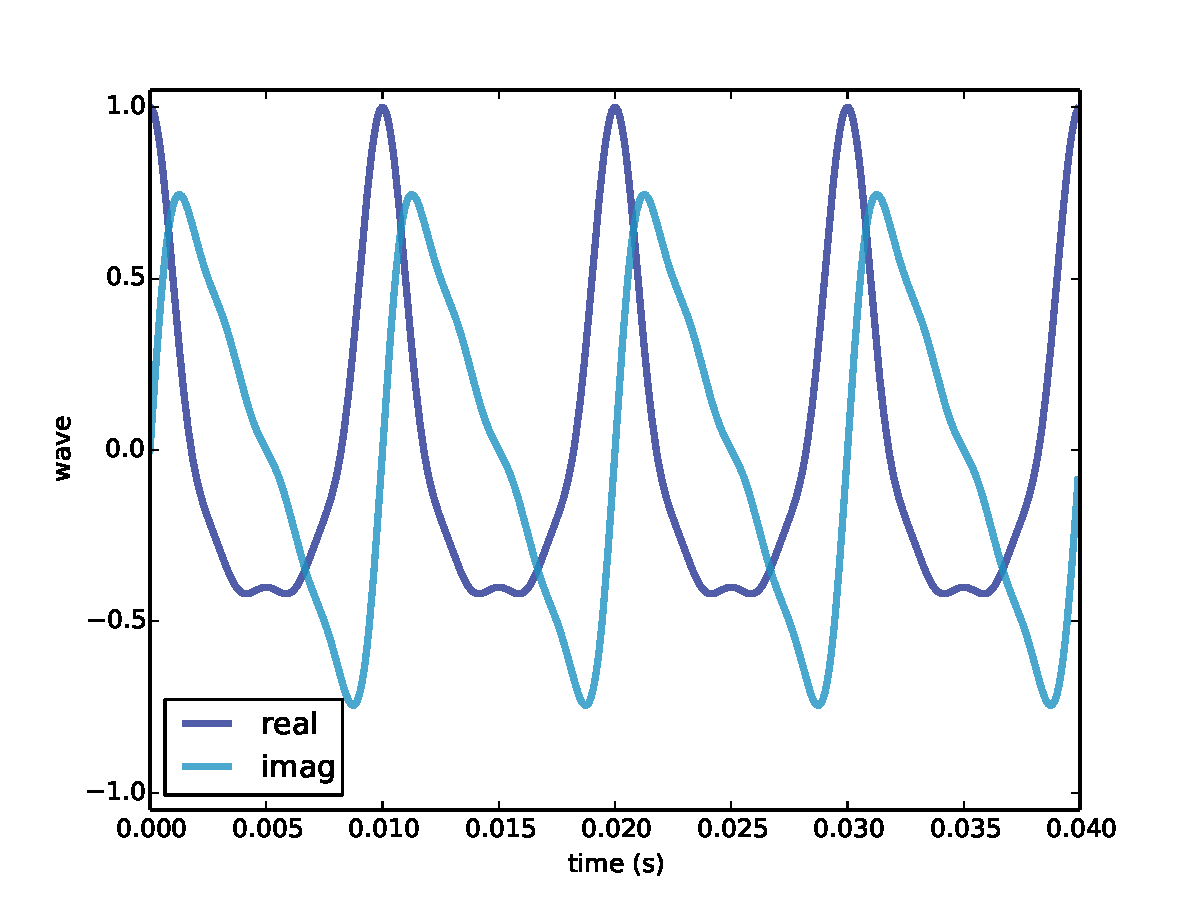
\includegraphics[height=2.5in]{figs/dft1.pdf}}
\caption{Real and imaginary parts of a mixture of complex sinusoids.}
\label{fig.dft1}
\end{figure}

So what is a complex signal?  I don't have a good answer to this
question.  The best I can offer is two bad, or maybe unsatisfying,
answers:

\begin{enumerate}

\item A complex signal is a mathematical abstraction that is
useful for computation and analysis, but it does not correspond
directly with anything in the real world.

\item You can think of a complex signal as a sequence of complex
numbers that contains two signals as its real and imaginary parts.

\end{enumerate}

Taking the second point of view, we can split the previous
signal into its real and imaginary parts:

\begin{verbatim}
    n = framerate / 25
    thinkplot.plot(ts[:n], ys[:n].real, label='real')
    thinkplot.plot(ts[:n], ys[:n].imag, label='imag')
\end{verbatim}

Figure~\ref{fig.dft1} shows a segment of the result.  The
real part is a sum of cosines; the imaginary part is
the sum of sines.  Although the waveforms look different, they
contain the same frequency components in the same proportions.
To our ears, they sound the same; in general, we don't hear
phase offsets.


\section{Synthesis with matrices}

As we saw in Section~\ref{synthesis}, we can also express the synthesis
problem in terms of matrix multiplication: 

\begin{verbatim}
PI2 = 2 * math.pi
i = complex(0, 1)

def synthesize2(amps, freqs, ts):
    args = numpy.outer(ts, freqs)
    M = numpy.exp(i * PI2 * args)
    ys = numpy.dot(M, amps)
    return ys
\end{verbatim}

Again, {\tt amps} is a NumPy array that contains a sequence
of amplitudes.

{\tt freqs} is a sequence containing the frequencies of the
components.  {\tt ts} contains the times where we will evaluate
the signal.

{\tt args} contains the outer product of {\tt ts} and {\tt freqs},
with the {\tt ts} running down the rows and the {\tt freqs}
running across the columns.

Each column of matrix {\tt M} contains a complex sinusoid with
a particular frequency, evaluated at a sequence of {\tt ts}.

When we multiply {\tt M} by the amplitudes, the result is a
vectors whose
elements correspond to the {\tt ts}; each element is the sum of
several complex sinusoids, evaluated at a particular time.

Here's the example from the previous section again:

\begin{verbatim}
>>> ys = synthesize2(amps, freqs, ts)
>>> print(ys)
[ 1.000 +0.000e+00j  0.995 +9.093e-02j  0.979 +1.803e-01j ...,
  0.979 -1.803e-01j  0.995 -9.093e-02j  1.000 -5.081e-15j]
\end{verbatim}

The result is the same.

In this example the amplitudes are real, but they could also be
complex.  What effect does a complex amplitude have on the result?
Remember that we can think of a complex number in two ways: either the
sum of a real and imaginary part, $x + i y$, or the product of a real
amplitude and a complex exponential, $A e^{i \phi_0}$.  Using the
second interpretation, we can see what happens when we multiply
a complex amplitude by a complex sinusoid.  For each frequency, $f$,
we have:
%
\[ A e^{i \phi_0} \cdot e^{i 2 \pi f t} = A e^{i 2 \pi f t + \phi_0} \]
%
In other words, the angle of the complex amplitude becomes
the phase offset of the complex sinusoid.

\begin{figure}
% dft.py
\centerline{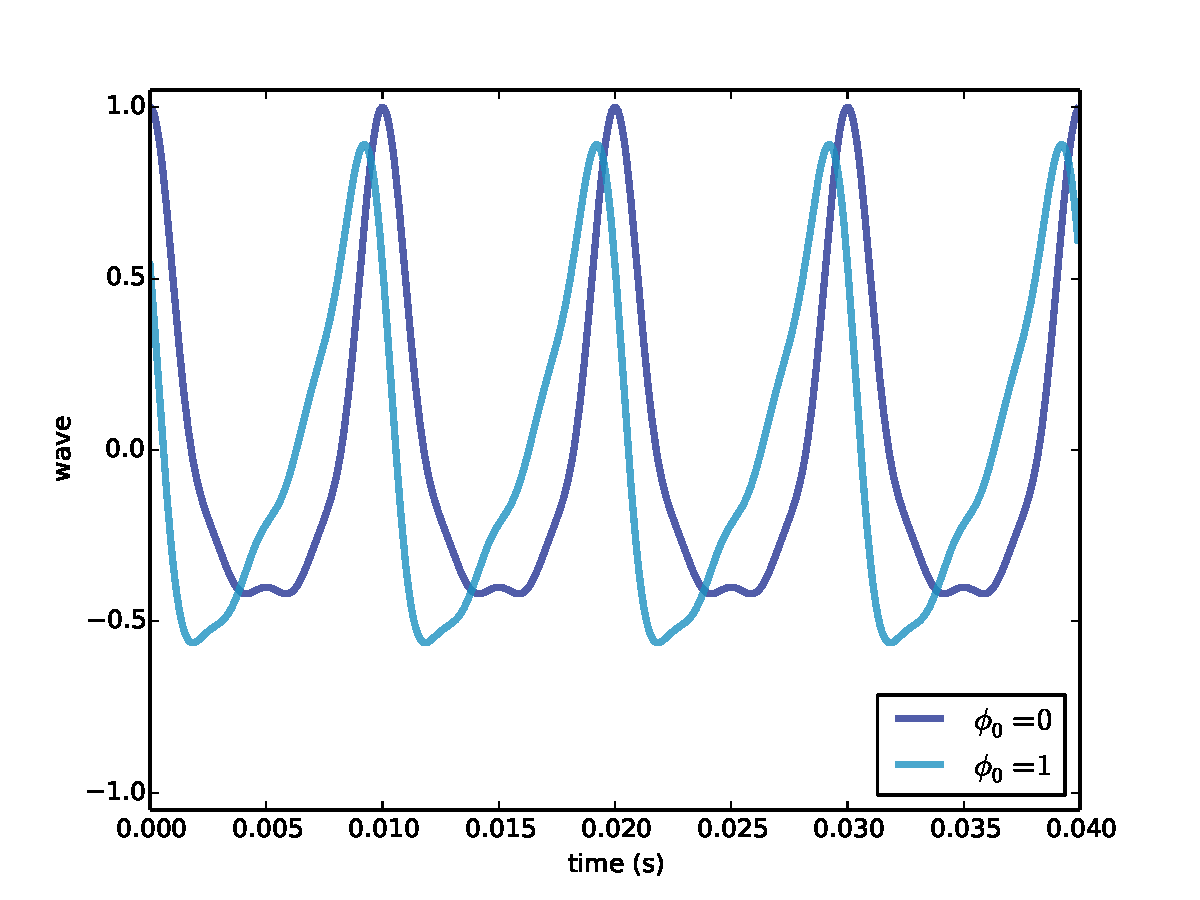
\includegraphics[height=2.5in]{figs/dft2.pdf}}
\caption{Real part of two complex signals that differ by a phase
offset.}
\label{fig.dft2}
\end{figure}

We can test that claim by running the previous example with
$\phi_0 = 1$ for all frequency components:

\begin{verbatim}
    amps2 = amps * numpy.exp(1j)
    ys2 = synthesize2(amps2, freqs, ts)

    thinkplot.plot(ts[:n], ys.real[:n], label=r'$\phi_0 = 0$')
    thinkplot.plot(ts[:n], ys2.real[:n], label=r'$\phi_0 = 1$')
\end{verbatim}

Figure~\ref{fig.dft2} shows the result.  The phase offset
$\phi_0 = 1$ shifts the wave to the left by about one sixth of
a cycle; it also changes the waveform, because the same phase
offset applied to different frequencies changes how the frequency
components line up with each other.

Now that we have the more general solution to the synthesis problem,
one that handles complex amplitudes, we are ready for the analysis
problem.



\section{The analysis problem}

The analysis problem is the inverse of the synthesis problem: given a
sequence of samples from a signal, $y$, and knowing the
frequencies that make up the signal, can we compute the
complex amplitudes of the components, $a$?

As we saw in Section~\ref{analysis}, we can solve this problem by forming
the synthesis matrix, $M$, and solving the system of linear
equations, $M a = y$ for $a$.

\begin{verbatim}
def analyze1(ys, freqs, ts):
    args = numpy.outer(ts, freqs)
    M = numpy.exp(i * PI2 * args)
    amps = numpy.linalg.solve(M, ys)
    return amps
\end{verbatim}

{\tt analyze1} takes a (possibly complex) wave array, {\tt ys}, a
sequence of real frequencies, {\tt freqs}, and a sequence of real
times, {\tt ts}.  It returns a sequence of complex amplitudes, {\tt
  amps}.

Continuing the previous example, we can confirm that {\tt analyze1}
can recover the amplitudes we started with.  For the linear system
solver to work, {\tt M} has to be square, so we need {\tt ys}, {\tt
  freqs} and {\tt ts} to have the same length.  I'll insure that by
slicing {\tt ys} and {\tt ts} down to the length of {\tt freqs}:

\begin{verbatim}
>>> n = len(freqs)
>>> amps2 = analyze1(ys[:n], freqs, ts[:n])
>>> print(amps2)
[ 0.60 +4.6e-13j  0.25 -1.4e-12j  0.10 +1.4e-12j  0.05 -4.6e-13j]
\end{verbatim}

Each component of {\tt amps} has a small imaginary part due to
floating-point errors, but the results are approximately correct.


\section{Efficient analysis}

Unfortunately, solving a linear system of equations is slow.  For the
DCT, we were able to speed things up by choosing {\tt freqs} and {\tt
  ts} so that {\tt M} is orthogonal.  That way, the inverse of {\tt M}
is the transpose of {\tt M}, and we can compute both DCT and inverse
DCT by matrix multiplication.

We'll do the same thing for the DFT, with one small change.
Since {\tt M} is complex, we need it to be {\bf unitary}, rather
than orthogonal, which means that the inverse of {\tt M} is
the conjugate transpose of {\tt M}, which we can compute by
transposing the matrix and negating the imaginary part of each
element.  See \url{http://en.wikipedia.org/wiki/Unitary_matrix}. 

The NumPy methods {\tt conj} and {\tt transpose} do what we
want.  Here's the code that computes {\tt M} for $N=4$ components:

\begin{verbatim}
N = 4
ts = numpy.arange(N) / N
freqs = numpy.arange(N)
args = numpy.outer(ts, freqs)
M = numpy.exp(i * PI2 * args)
print(M)
\end{verbatim}

If $M$ is unitary, $M*M = I$, where $M*$ is the conjugate transpose
of $M$, and $I$ is the identity matrix.  We can test whether $M$
is unitary like this:

\begin{verbatim}
MstarM = M.conj().transpose().dot(M)
print(MstarM)
\end{verbatim}

The result, within the tolerance of floating-point error, is
$4 I$, so $M$ is unitary except for an extra factor of $N$,
similar to the extra factor of 2 we found with the DCT.

So we can use this result to write a faster version of
{\tt analyze1}:

\begin{verbatim}
def analyze2(ys, freqs, ts):
    args = numpy.outer(ts, freqs)
    M = numpy.exp(i * PI2 * args)
    amps = M.conj().transpose().dot(ys) / N
    return amps
\end{verbatim}

And test it with appropriate values of {\tt freqs} and {\tt ts}:

\begin{verbatim}
>>> N = 4
>>> amps = numpy.array([0.6, 0.25, 0.1, 0.05])
>>> freqs = numpy.arange(N)
>>> ts = numpy.arange(N) / N
>>> ys = synthesize2(amps, freqs, ts)

>>> amps2 = analyze2(ys, freqs, ts)
>>> print(amps2)
[ 0.60 +2.1e-17j  0.25 +1.3e-17j  0.10 -3.9e-17j  0.05 -8.3e-17j]
\end{verbatim}

Again, the result is correct within the tolerance of floating-point
arithmetic.

\section{DFT}

As a function, {\tt analyze2} would be hard to use because it
only works if {\tt freqs} and {\tt ts} are chosen correctly.  So
the usual definition of {\tt dft} takes {\tt ys} and computes
{\tt freqs} and {\tt ts} accordingly:

\begin{verbatim}
def dft(ys):
    N = len(ys)
    ts = numpy.arange(N) / N
    freqs = numpy.arange(N)
    args = numpy.outer(ts, freqs)
    M = numpy.exp(i * PI2 * args)
    amps = M.conj().transpose().dot(ys)
    return amps
\end{verbatim}

Notice that I made one small change; this version of {\tt DFT}
does not divide through by {\tt N}.  I did that to make it
consistent with the conventional definition of DFT.  Here's my
version:

\begin{verbatim}
>>> print(dft(ys))
[ 2.4 +8.3e-17j  1.0 +5.6e-17j  0.4 -1.6e-16j  0.2 -3.3e-16j]
\end{verbatim}

And here's the version in {\tt numpy.fft}:

\begin{verbatim}
>>> print(numpy.fft.fft(ys))
[ 2.4 +8.0e-17j  1.0 -2.5e-17j  0.4 -3.1e-17j  0.2 -2.5e-17j]
\end{verbatim}

They are approximately the same.

The inverse DFT is almost the same, except {\em now} we have to
divide through by N:

\begin{verbatim}
def idft(amps):
    ys = dft(amps) / N
    return ys
\end{verbatim}

Finally, we can confirm that {\tt dft(idft(amps))} yields {\tt amps}.

\begin{verbatim}
>>> ys = idft(amps)
>>> print(dft(ys))
[ 0.60 -2.1e-17j  0.05 +0.0e+00j  0.10 -2.5e-17j  0.25 -1.4e-17j]
\end{verbatim}

If I could go back in time, I might change the definition of
DFT so it divides by $N$ and the inverse DFT doesn't.  That would
be more consistent my presentation of the synthesis and analysis
problems.

Or I might change the definition so that both operations divide
through by $\sqrt{N}$.  Then the DFT and inverse DFT would be
identical.

I can't go back in time (yet!), so we're stuck with a slightly
weird convention.  But for practical purposes it doesn't really
matter.


\section{Just one more thing}

\begin{figure}
% dft.py
\centerline{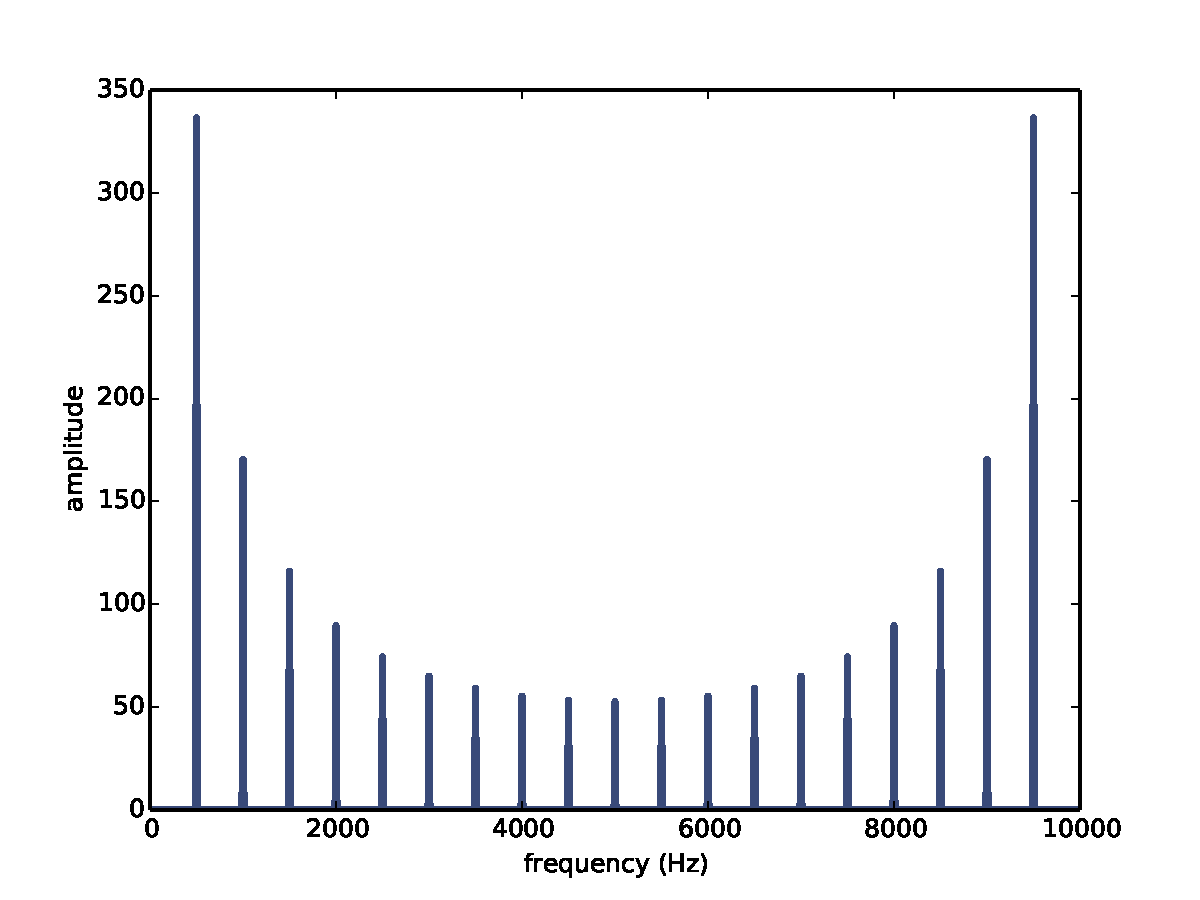
\includegraphics[height=2.5in]{figs/dft3.pdf}}
\caption{DFT of a 500 Hz sawtooth signal sampled at 10 kHz.}
\label{fig.dft3}
\end{figure}

The Spectrum class in {\tt thinkdsp} is based on {\tt numpy.ftt.rfft},
which computes the ``real FFT''; that is, it works with real signals.
The DFT is more general than the real FFT; it works with complex
signals.

So what happens when we apply DFT to a real signal?  Let's look at
an example:

\begin{verbatim}
    framerate = 10000
    signal = thinkdsp.SawtoothSignal(freq=500)
    wave = signal.make_wave(duration=0.1, framerate=framerate)
    hs = dft(wave.ys)
    amps = numpy.absolute(hs)
\end{verbatim}

This code makes a sawtooth wave with frequency 500 Hz, sampled at
framerate 10 kHz.  {\tt hs} contains the complex DFT of the wave;
{\tt amps} contains the amplitude at each frequency.  But what
frequency do these amplitudes correspond to.  If we look at the
body of {\tt dft}, we see:

\begin{verbatim}
    fs = numpy.arange(N)
\end{verbatim}

So it's tempting to think that these values are the right frequencies.
The problem is that {\tt dft} doesn't know the sampling rate.  The
DFT assumes that the duration of the wave is 1 time unit, so the sampling
rate is $N$ per time unit.  In order to interpret the frequencies,
we have to convert from these arbitrary time units back to seconds,
like this:

\begin{verbatim}
    fs = numpy.arange(N) * framerate / N
\end{verbatim}

With this change, the range of frequencies is from 0 to the actual
framerate, 10 kHz.  Now we can plot the spectrum:

\begin{verbatim}
    thinkplot.plot(fs, amps)
    thinkplot.config(xlabel='frequency (Hz)', 
                     ylabel='amplitude')
\end{verbatim}

Figure~\ref{fig.dft3} shows the amplitude of the signal for each
frequency component from 0 to 1 kHz.  The left half of the figure
is what we should expect: the dominant frequency is at 500 Hz, with
harmonics dropping off like $1/f$.

But the right half of the figure is a surprise.  Past 5000 Hz, the
amplitude of the harmonics start growing again, peaking at 9500 Hz.
What's going on?

The answer: aliasing.  Remember that with framerate 10000 Hz, the
folding frequency is 5000 Hz.  As we saw in Section~\ref{aliasing}
a component at 5500 Hz is indistinguishable from a component
at 4500 Hz.  So when we evaluate the DFT at 5500 Hz, we get the same
value as at 4500 Hz.  Similarly, the value at 6000 Hz is the same
as the one at 4000 Hz, and so on.

So the DFT of a real signal is symmetric around the folding frequency.
Since there is no additional information past this point, we can
save time be evaluating only the first half of the DFT,
and that's exactly what {\tt rfft} does.


\section{Exercises}

\begin{exercise}
In this chapter, I showed how we can express the DFT and inverse
DFT as matrix multiplications.  These operations are relatively
fast, taking time proportional to $N^2$, where $N$ is the length
of the wave array.  And that would be fast enough for many applications,
but it turns out that there is a faster algorithm, the
Fast Fourier Transform (FFT), which takes time proportional to 
$N \log N$.

Read about the FFT at
\url{http://en.wikipedia.org/wiki/Cooley-Tukey_FFT_algorithm}, and
write an implementation.  Hint: I suggest you write a simple version
as a recursive function; don't worry about ``data reordering, bit
reversal, and in-place algorithms.''
\end{exercise}


\chapter{Filtering and Convolution}

In this chapter I present one of the most important and useful
ideas related to signal processing: the Convolution Theorem.
Before we can understand the Convolution Theorem, we have to understand
convolution.  I'll start with one of the simplest examples: smoothing.

Then we'll see how the Convolution Theorem works and, for
those who are interested, I'll try to explain {\em why} it works.

The code for this chapter is in {\tt convolution.py}, which is in the
repository for this book (see Section~\ref{code}).


\section{Smoothing}

\begin{figure}
% convolution1.py
\centerline{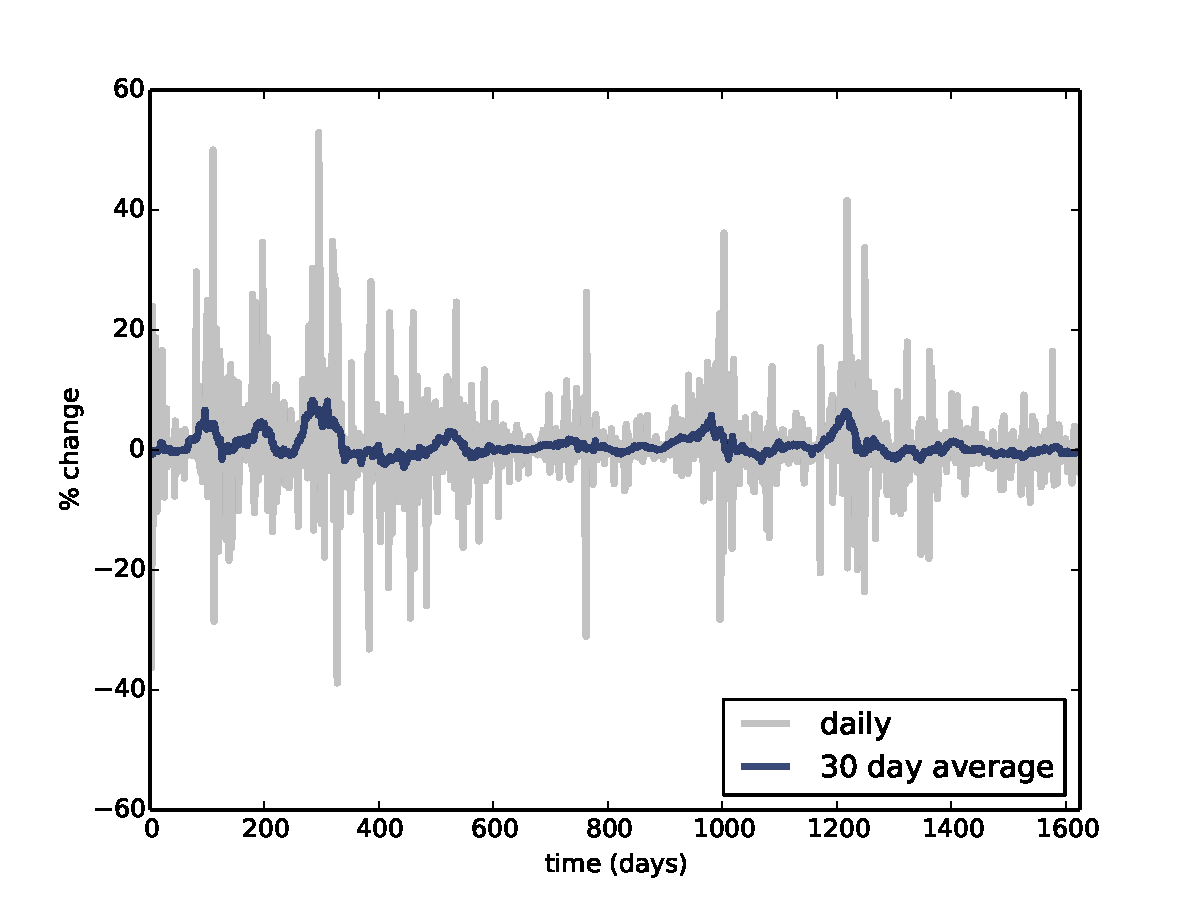
\includegraphics[height=2.5in]{figs/convolution1.pdf}}
\caption{Daily changes in the price of BitCoin and a 30-day moving
average.}
\label{fig.convolution1}
\end{figure}


Smoothing is an operation that tries to remove short-term variations
from a signal in order to reveal long-term trends.  For example, if
you plot daily changes in the price of a stock, it would look noisy;
a smoothing operator might make it easier to see whether the price
was generally going up or down over time.  

A common smoothing algorithm is a moving average, which computes
the mean of the previous $n$ values, for some value of $n$.

For example, Figure~\ref{fig.convolution1} shows the daily percent
change in the price of BitCoin from July 18, 2010 to December 28,
2014 (downloaded from \url{http://www.coindesk.com}).  The gray line
is the raw data, the darker line shows the 30-day moving average.
In the short term, the price of BitCoin is quite volatile, often
changing by more than 10\% in a day.  Smoothing removes the most
extreme changes and makes it easier to see long-term trends.

Smoothing operations also apply to sound signals.  As an example,
I'll start with a square wave at 440 Hz.  As we saw in Section~\ref{},
the harmonics of a square wave drop off slowly, so it contains many
high-frequency components.

\begin{verbatim}
    signal = thinkdsp.SquareSignal(freq=440)
    wave = signal.make_wave(duration=1, framerate=44100)
    segment = wave.segment(duration=0.01)
\end{verbatim}

{\tt wave} is a 1-second segment of the signal; {\tt segment}
is a shorter segment I'll use for plotting.

You can try out this example, and listen to it, in
{\tt chap08.ipynb}, which is in the repository for this
book and also available at \url{http://tinyurl.com/thinkdsp08}.

To compute the moving average of this signal, I'll create
a window with 11 elements and normalize it so the elements
add up to 1.

\begin{verbatim}
    window = numpy.ones(11)
    window /= sum(window)
\end{verbatim}

Now I can compute the average of the first 11 elements by
multiplying the window by the wave array:

\begin{verbatim}
    padded = zero_pad(window, len(segment))
    prod = padded * segment.ys
\end{verbatim}

{\tt padded} is a version of the window with zeros added to
the end so it has the same length as {\tt segment.ys}
(\verb"zero_pad" is defined in {\tt convolution.py}).
{\tt prod} is the product of the window and the wave array.

The first 11 elements of this wave array are -1, so their
average is -1, and (sure enough) that's the value of {\tt prod}.

To compute the next element of the smoothed signal, we shift
the right and compute the average of 11 elements of the wave
array, starting with the second.

\begin{figure}
% convolution2.py
\centerline{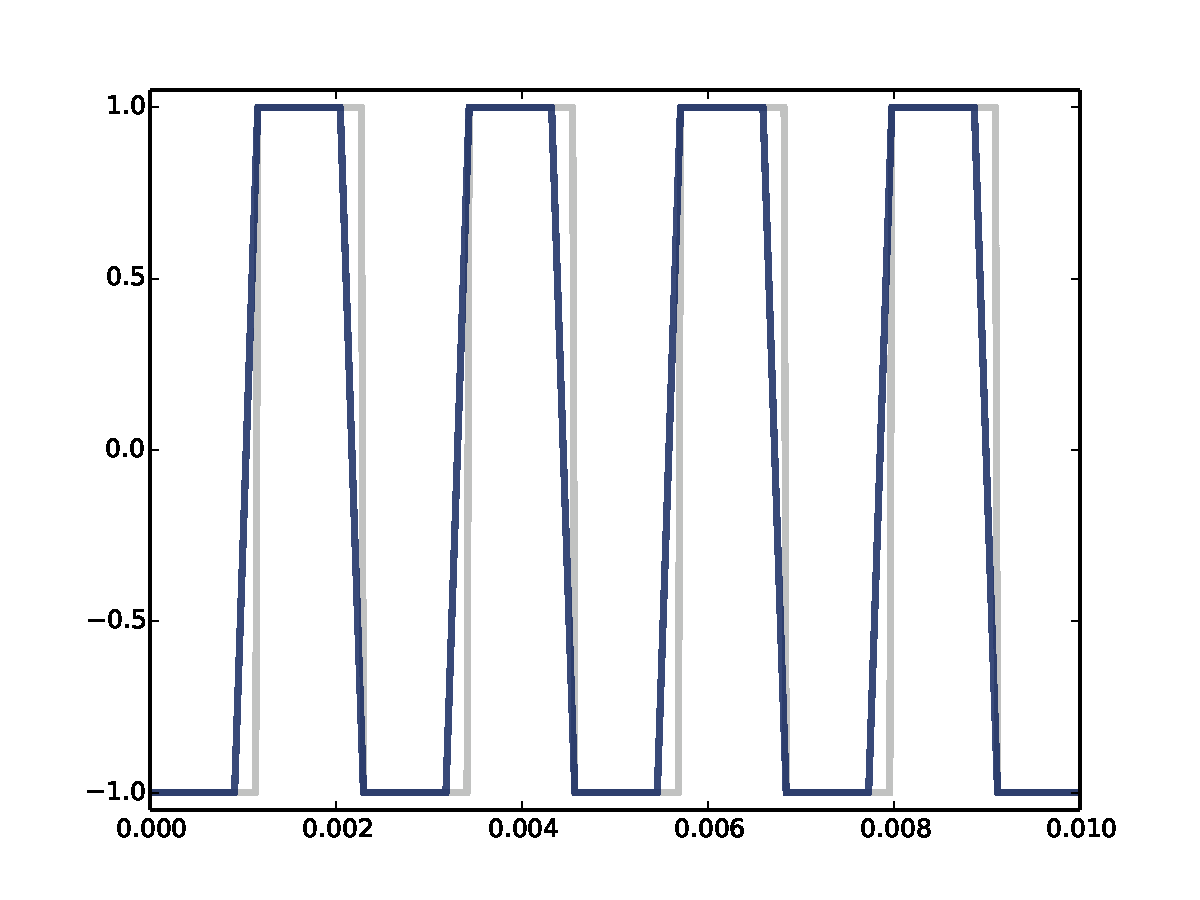
\includegraphics[height=2.5in]{figs/convolution2.pdf}}
\caption{A square signal at 400 Hz (gray) and an 11-element
moving average (darker).}
\label{fig.convolution2}
\end{figure}


The following code computes the rolling average for the whole
wave:

\begin{verbatim}
    smoothed = numpy.zeros_like(segment.ys)
    rolled = padded
    for i in range(len(segment.ys)):
        smoothed[i] = sum(rolled * segment.ys)
        rolled = numpy.roll(rolled, 1)
\end{verbatim}

{\tt smoothed} is the wave array where I store the results.
{\tt rolled} is a copy of {\tt padded} that gets shifted to
the right by one element each time through the loop.  Inside
the loop, we multiply the segment by {\tt rolled} to select
11 elements, and then add them up.

Figure~\ref{fig.convolution2} shows the result.  The gray line
is the original signal; the darker line is the smoothed signal.
The smoothed signal starts to ramp up when the leading edge of
the window reaches the first transition, and levels off when
the window crosses the transition.  As a result, the transitions
are less abrupt, and the corners less sharp.  If you listen
to the smoothed signal, it sounds less buzzy and slightly muffled.


\section{Convolution}
\label{convolution}

The operation we just computed is called {\bf convolution},
and it is such a common operation that NumPy provides an
implementation that is simpler and faster than my version:

\begin{verbatim}
    ys = numpy.convolve(segment.ys, window, mode='valid')
    smooth2 = thinkdsp.Wave(ys, framerate=wave.framerate)
\end{verbatim}

{\tt numpy.convolve} computes the convolution of the wave
array and the window.  The mode flag {\tt valid} indicates
that it should only compute values when the window and the
wave array overlap completely, so it stops when the right
edge of the window reaches the end of the wave array.  Other
than that, the result is the same as in Figure~\ref{fig.convolution2}.

\newcommand{\conv}{\ast}

Actually, there is one other difference.  The loop in the
previous section actually computes {\bf cross-correlation}:
%
\[ (f \star g)[i] = \sum_{j=0}^{N-1} f[j] g[j-i]  \]
%
where $f$ is a wave array with length $N$, $g$ is the window,
and $\star$ is the symbol for cross-correlation.  To
compute the $i$th element of the result, we shift $g$ to
the right, which is why the index is $j-i$.

The mathematical definition of convolution is slightly different:
%
\[ (f \conv g)[i] = \sum_{j=0}^{N-1} f[j] g[i-j]  \]
%
The symbol $\conv$ represents convolution.  The difference is
that the index of $g$ has been negated, which has the same
effect as reversing the elements of $g$ (assuming that negative
indices wrap around to the end of the array).

Because the window we are using is symmetric,
cross-correlation and convolution yield the same result.
When we use other windows, we will have to be more careful.

You might wonder why convolution is defined the way it is.
I can't answer that question yet, but I will, in
Section~\ref{whyflip}.


\section{The frequency domain}

\begin{figure}
% convolution4.py
\centerline{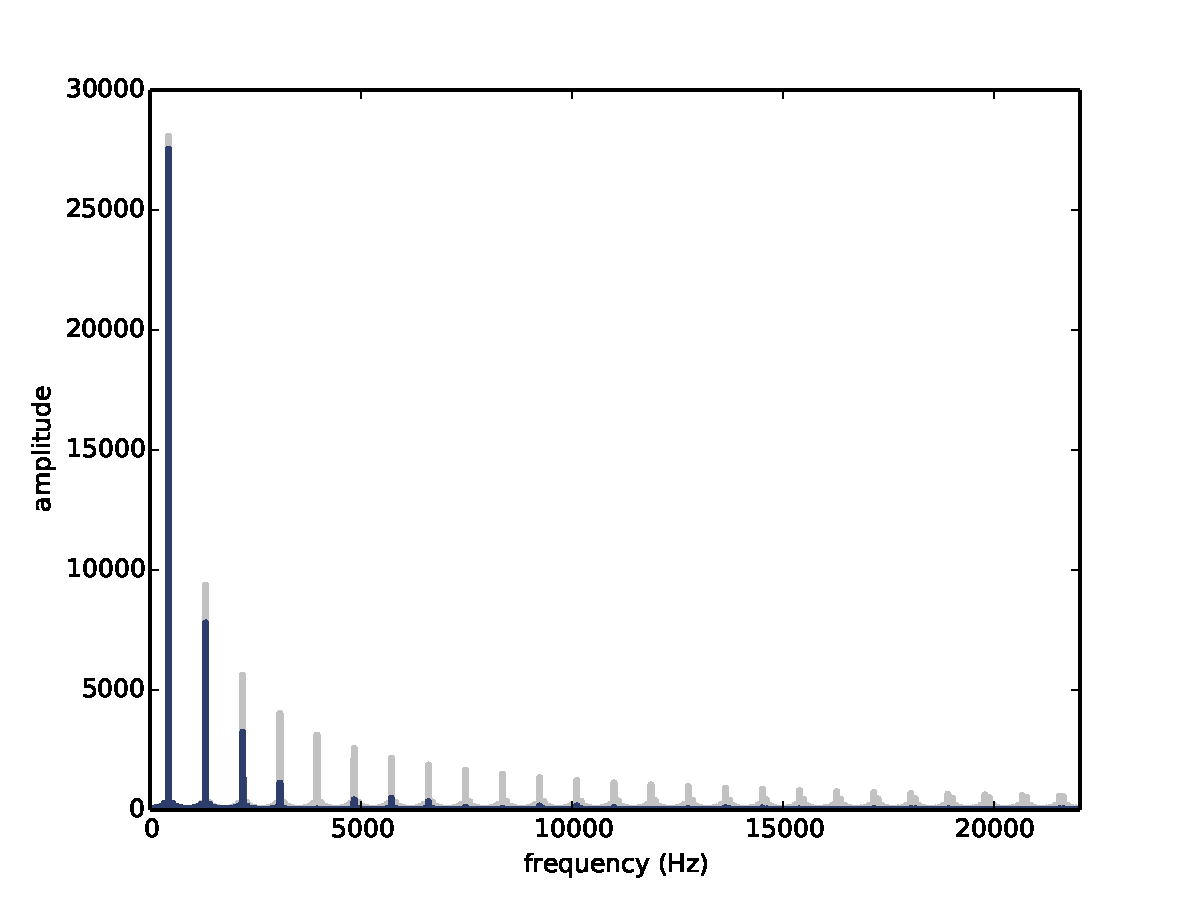
\includegraphics[height=2.5in]{figs/convolution4.pdf}}
\caption{Spectrum of the square wave before and after smoothing.}
\label{fig.convolution4}
\end{figure}

Smoothing makes the transitions in a square signal less abrupt,
and makes the sound slightly muffled.  Let's see what effect this
operation has on the spectrum.  First I'll plot the spectrum
of the original wave:

\begin{verbatim}
    spectrum = wave.make_spectrum()
    spectrum.plot(color='0.7')
\end{verbatim}

Then the smoothed wave:

\begin{verbatim}
    ys = numpy.convolve(wave.ys, window, mode='same')
    smooth = thinkdsp.Wave(ys, framerate=wave.framerate)
    spectrum2 = smooth.make_spectrum()
    spectrum2.plot()
\end{verbatim}

Figure~\ref{fig.convolution4} shows the result.  The fundamental
frequency is almost unchanged; the first few harmonics are
attenuated, and the higher harmonics are almost eliminated.  So
smoothing has the effect of a low-pass filter, which we
saw in Section~\ref{spectrums} and Section~\ref{pink}.

To see how much each component has been attenuated, we can
compute the ratio of the two spectrums:

\begin{verbatim}
    amps = spectrum.amps
    amps2 = spectrum2.amps
    ratio = amps2 / amps    
    ratio[amps<560] = 0
    thinkplot.plot(ratio)
\end{verbatim}

{\tt ratio} is the ratio of the amplitude before and after 
smoothing.  When {\tt amps} is small, this ratio can be big
and noisy, so for simplicity I set the ratio to 0 except for
where the harmonics are.

\begin{figure}
% convolution5.py
\centerline{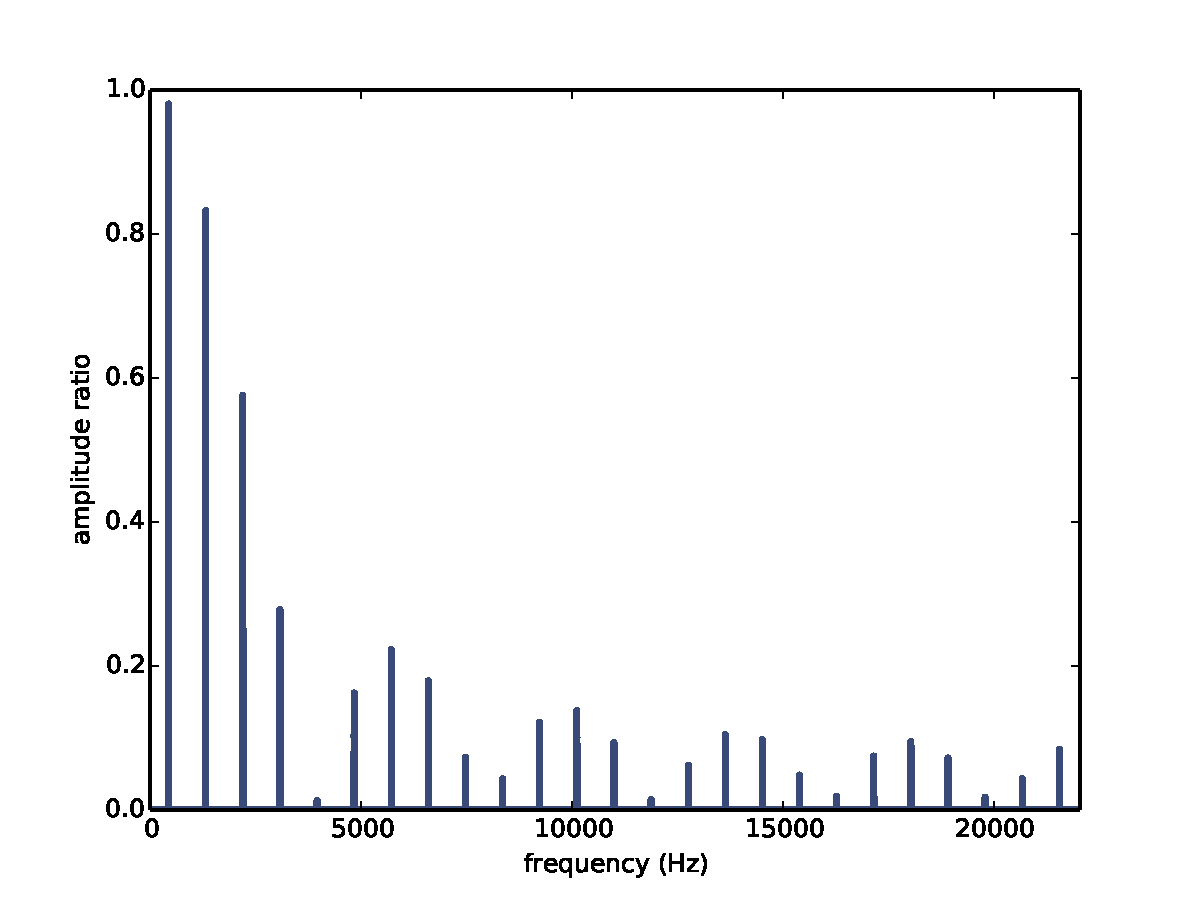
\includegraphics[height=2.5in]{figs/convolution5.pdf}}
\caption{Ratio of spectrums for the square wave, before and after smoothing.}
\label{fig.convolution5}
\end{figure}

Figure~\ref{fig.convolution5} shows the result.  As expected, the
ratio is high for low frequencies and drops off at a cutoff frequency
near 4000 Hz.  But there is another feature we did not expect: above
the cutoff, the ratio seems to oscillate between 0 and 0.2.
What's up with that?


\section{The convolution theorem}

\begin{figure}
% convolution6.py
\centerline{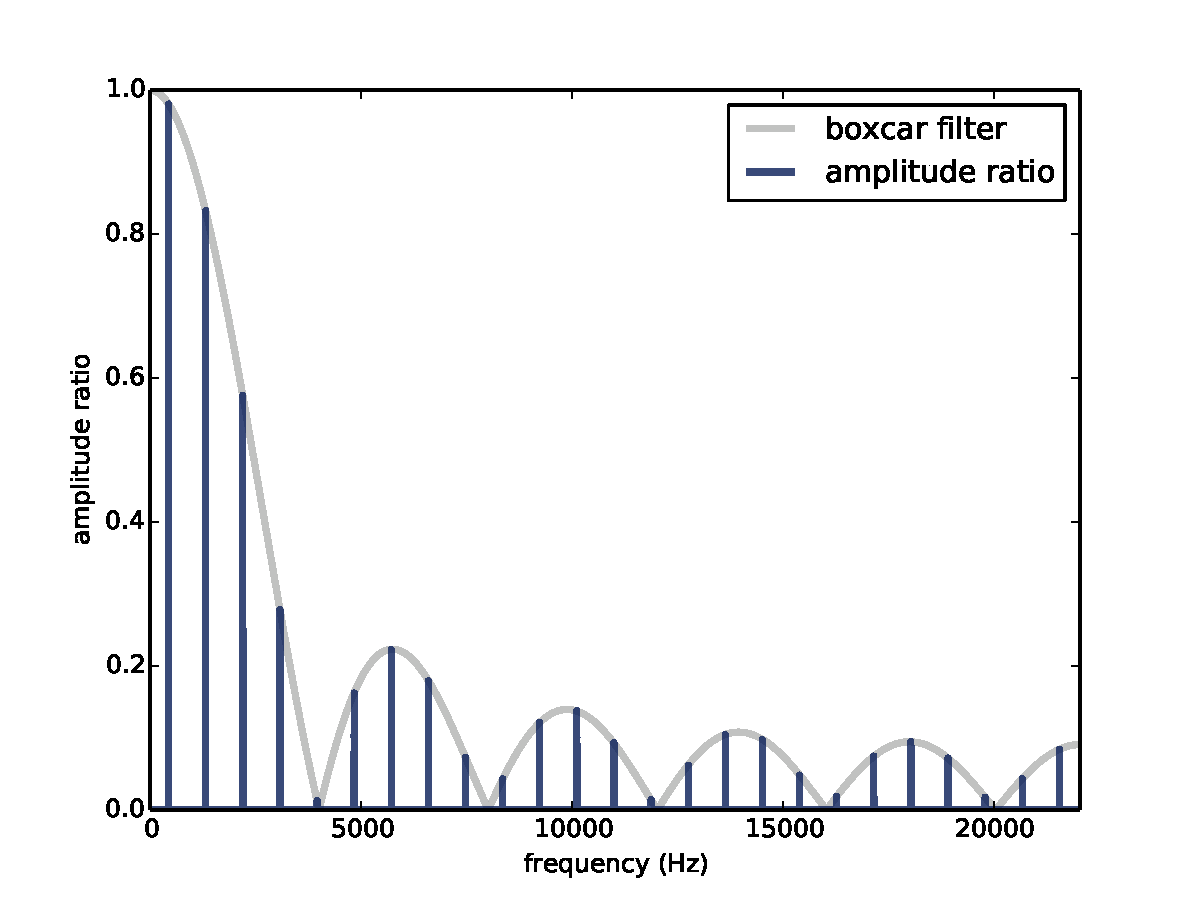
\includegraphics[height=2.5in]{figs/convolution6.pdf}}
\caption{Ratio of spectrums for the square wave, before and after
  smoothing, along with the DFT of the smoothing window.}
\label{fig.convolution6}
\end{figure}

The answer is the convolution theorem.  Stated mathematically:
%
\[ DFT(f \conv g) = DFT(f) \cdot DFT(g) \]
%
where $f$ is a wave array and $g$ is a window.  In words,
the convolution theorem says that if we convolve $f$ and $g$,
and then compute the DFT, we get the same answer as computing
the DFT of $f$ and $g$, and then multiplying the results
element-wise.  Or, more concisely, convolution in the time
domain corresponds to multiplication in the frequency domain.

And that explains Figure~\ref{fig.convolution5}, because when we
convolve a wave and a window, we multiply the spectrum of
the wave with the spectrum of the window.  To see how that works,
we can compute the DFT of the window:

\begin{verbatim}
    padded = zero_pad(window, len(wave))
    dft_window = numpy.fft.rfft(padded)
    thinkplot.plot(abs(dft_window))
\end{verbatim}

{\tt padded} contains the window, padded with zeros to be the
same length as {\tt wave}.  \verb"dft_window" contains the
DFT of the smoothing window.

Figure~\ref{fig.convolution6} shows the result, along with the
ratios we computed in the previous section.  The ratios are
exactly the amplitudes \verb"dft_window".  Mathematically:
%
\[ |DFT(f \conv g)| / |DFT(f)| = |DFT(g)| \]
%
where $|z|$ represents the amplitude of a complex number $z$.

In this context, the DFT of a window is called a {\bf filter}.
For any convolution window in the time domain, there is a
corresponding filter in the frequency domain.  And for any
filter than can be expressed by element-wise multiplication in
the frequency domain, there is a corresponding window.


\section{Gaussian filter}

\begin{figure}
% convolution7.py
\centerline{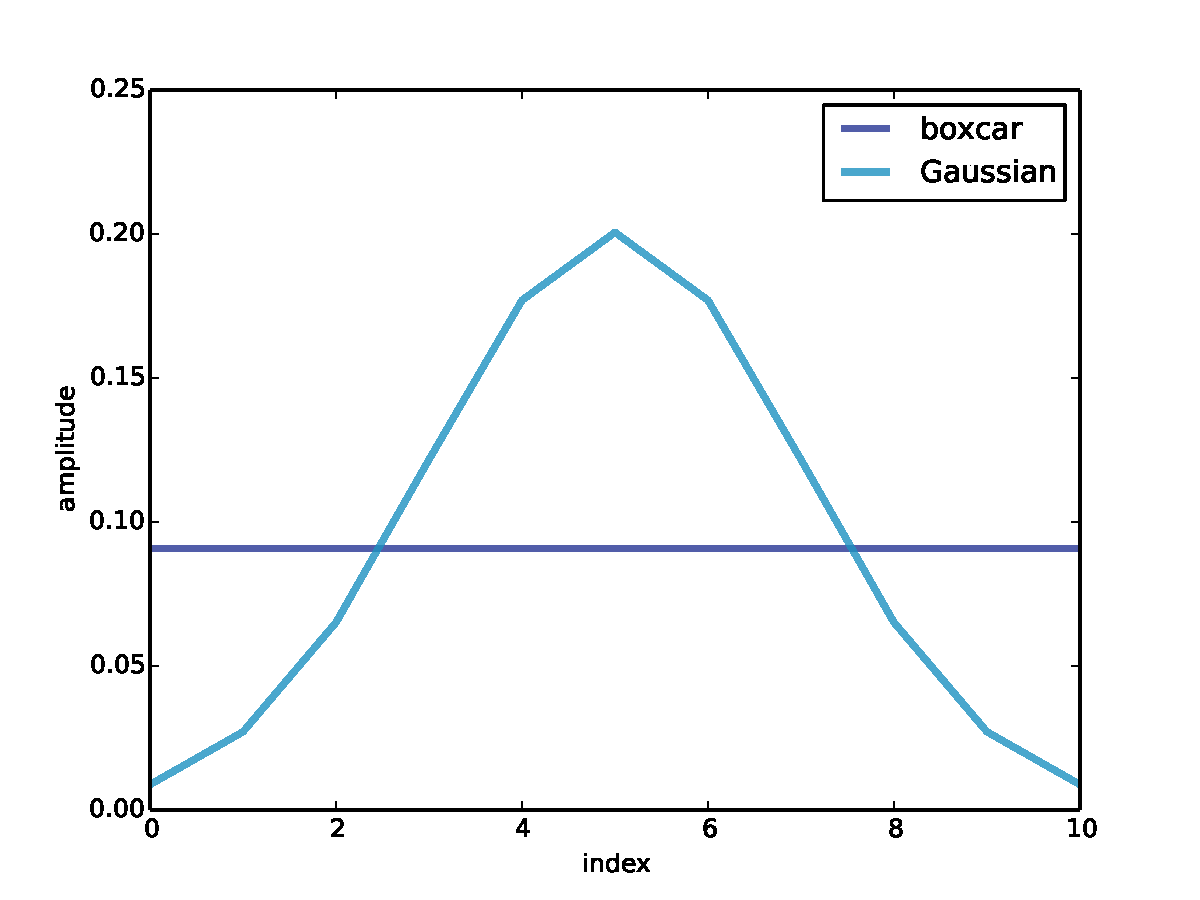
\includegraphics[height=2.5in]{figs/convolution7.pdf}}
\caption{Boxcar and Gaussian windows.}
\label{fig.convolution7}
\end{figure}

The moving average window we used in the previous section is
a low-pass filter, but it is not a very good one.  It cuts off
at around 4000 Hz, but then it bounces around for a while.  
For reasons we will see soon, we can do better with
a Gaussian window.

SciPy provides functions that compute many common convolution
windows, including {\tt gaussian}:

\begin{verbatim}
    gaussian = scipy.signal.gaussian(M=11, std=2)
    gaussian /= sum(gaussian)
\end{verbatim}

{\tt M} is the number of elements in the window; {\tt std}
is the standard deviation of the Gaussian expression used to
compute it.  Figure~\ref{fig.convolution7} shows the shape
of the window.  It is a discrete approximation of the Gaussian
``bell curve''.  The figure also shows the moving average window
from the previous example, which is sometimes called a
``boxcar'' window because it looks like a rectangular railway car.

\begin{figure}
% convolution.py
\centerline{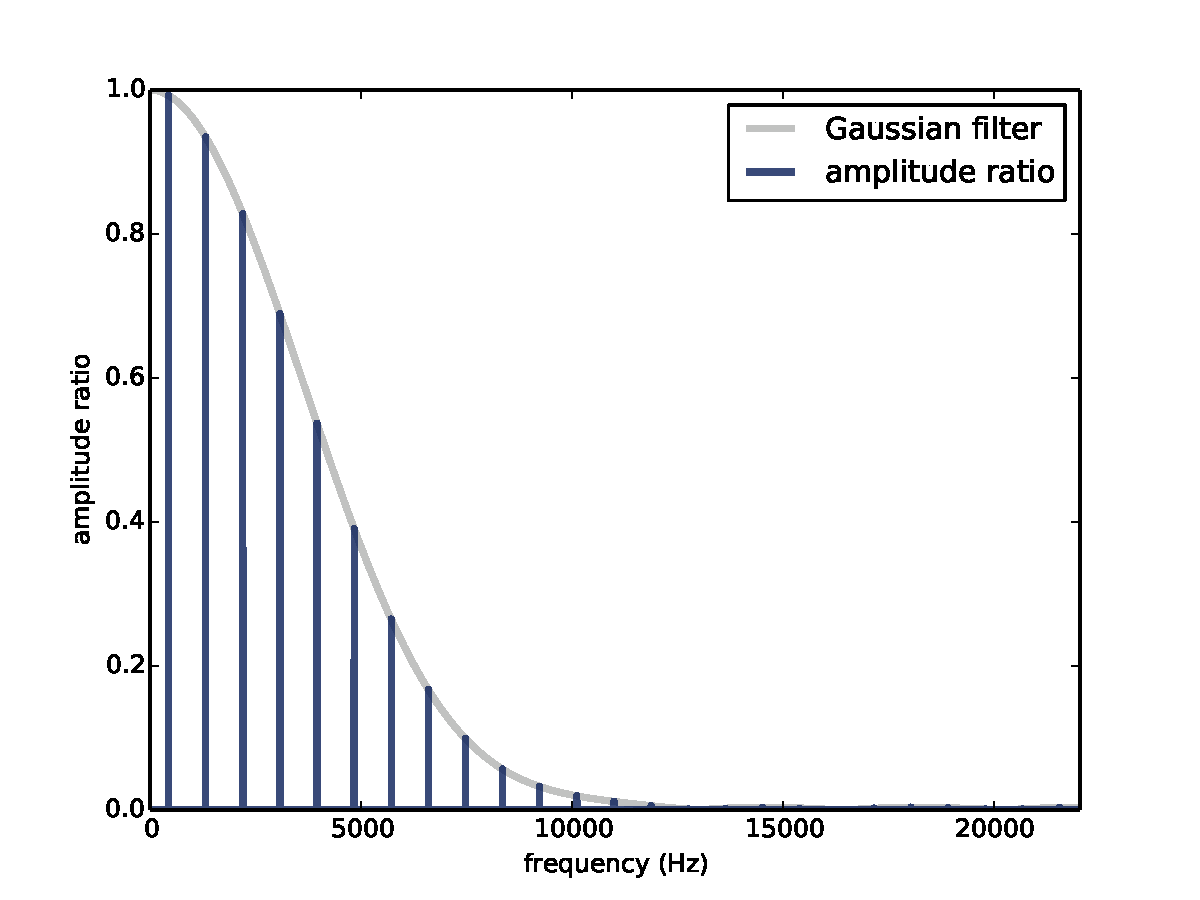
\includegraphics[height=2.5in]{figs/convolution8.pdf}}
\caption{Ratio of spectrums before and after Gaussian smoothing, and
  the DFT of the window.}
\label{fig.convolution8}
\end{figure}

I ran the computations from the previous sections again
with this curve, and generated Figure~\ref{fig.convolution8},
which shows the ratio of the spectrums before and after
smoothing, along with the DFT of the Gaussian window. 

As a low-pass filter, Gaussian smoothing is much better than
a simple moving average.  The cutoff frequency is a little
higher; near 7000 Hz, the ratio is 0.1.  But above that, the
ratio drops quickly and stays low, with almost none of the oscillation we
saw with the boxcar window.

In Figure~\ref{fig.convolution8}, the shape of the filter
might look familiar.  As it turns out, the DFT of a Gaussian
curve is also a Gaussian curve.  In this example, the
window is a discrete approximation, so the resulting filter
is only approximately Gaussian.


\section{Efficient convolution}

One of the reasons the FFT is such an important algorithm is that,
combined with the Convolution Theorem, it provides an efficient
way to compute convolution, cross-correlation, and autocorrelation.

Again, the Convolution Theorem states
%
\[ DFT(f \conv g) = DFT(f) \cdot DFT(g) \]
%
So one way to compute a convolution is:
%
\[ f \conv g = IDFT(DFT(f) \cdot DFT(g)) \]
%
where $IDFT$ is the inverse DFT.  A simple implementation of
convolution takes time proportional to $N^2$; this algorithm,
using FFT, takes time proportional to $N \log N$.

We can confirm that it works by computing the same convolution
both ways.  As an example, I'll apply it to the BitCoin data
shown in Figure~\ref{fig.convolution1}.

\begin{verbatim}
    df = pandas.read_csv('coindesk-bpi-USD-close.csv', 
                         nrows=1625, 
                         parse_dates=[0])
    ys = df.Close.values
\end{verbatim}

This example uses Pandas to read the data from the CSV file (included
in the repository for this book).  If you are not familiar with
Pandas, don't worry: I'm not going to do much with it in this book.
But if you are interested, you can learn more about it in
{\it Think Stats} at \url{http://thinkstats2.com}.

The result, {\tt df}, is a DataFrame, one of the data structures
provided by Pandas.  {\tt ys} is a NumPy array that contains daily
closing prices.

Next I'll create a Gaussian window and convolve it with {\tt ys}:

\begin{verbatim}
    window = scipy.signal.gaussian(M=30, std=6)
    window /= window.sum()
    smoothed = numpy.convolve(ys, window, mode='valid')
\end{verbatim}

With {\tt mode='valid'}, {\tt numpy.convolve} returns values
only where the window and the signal overlap completely, avoiding
bogus values at the beginning and end.

\verb"fft_convolve" computes the same thing using FFT:

\begin{verbatim}
def fft_convolve(signal, window):
    fft_signal = numpy.fft.fft(signal)
    fft_window = numpy.fft.fft(window)
    return numpy.fft.ifft(fft_signal * fft_window)
\end{verbatim}

We can test it by padding the window to the same length
as {\tt ys}:

\begin{verbatim}
    padded = zero_pad(window, len(ys))
    smoothed2 = fft_convolve(ys, padded)
\end{verbatim}

The result has $M-1$ bogus values at the beginning, where
$M$ is the length of the window.  If we slice off the bogus
values, we the same result as before, with about 12 digits
of precision.

\begin{verbatim}
    M = len(window)
    smoothed2 = smoothed2[M-1:]
\end{verbatim}

You can run this example in
{\tt chap08.ipynb}, which is in the repository for this
book and also available at \url{http://tinyurl.com/thinkdsp08}.


\section{Efficient autocorrelation}

\begin{figure}
% convolution.py
\centerline{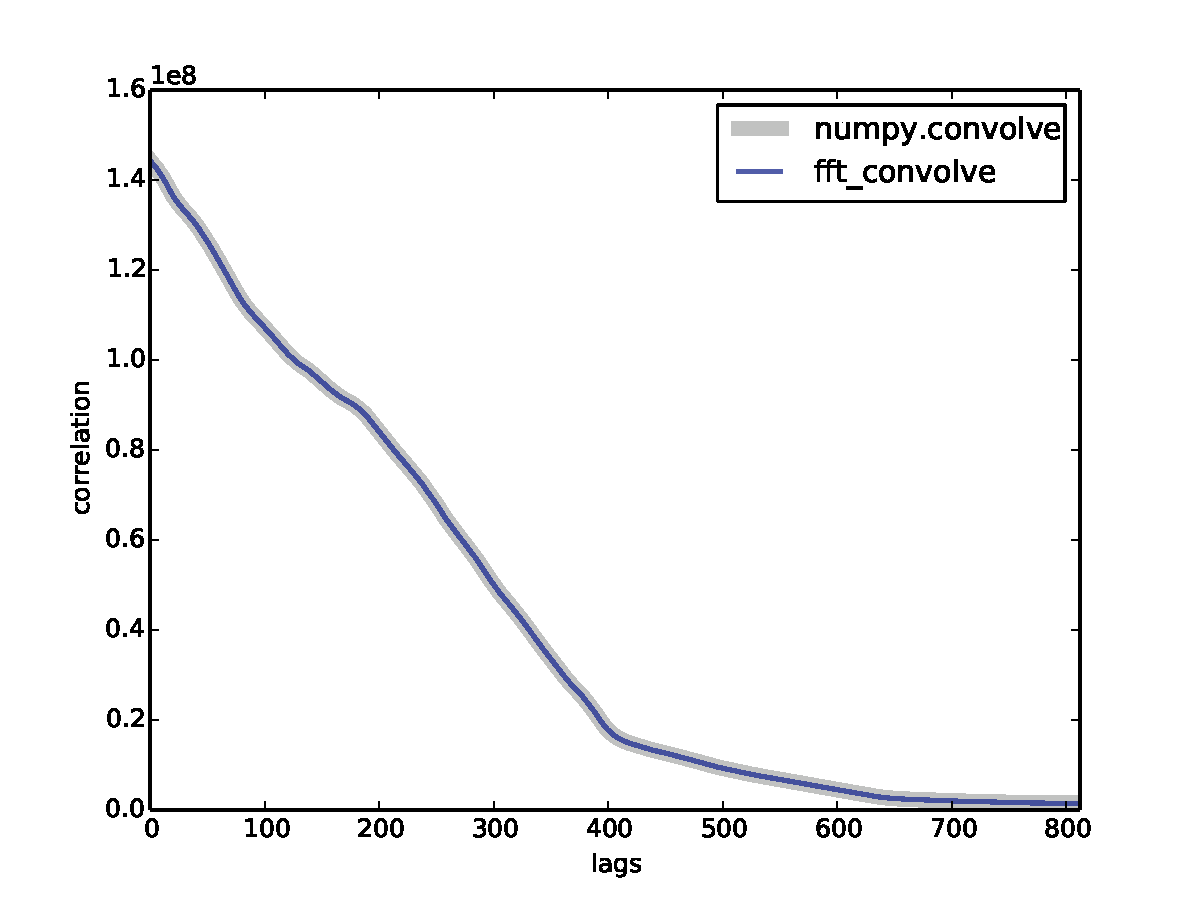
\includegraphics[height=2.5in]{figs/convolution9.pdf}}
\caption{Autocorrelation functions computed by NumPy and
  {\tt fft\_correlate}.}
\label{fig.convolution9}
\end{figure}

In Section~\ref{convolution} I presented the definition of
cross-correlation and convolution, and we saw that they are
almost the same, except that in convolution the window is
reversed (for reasons we are still waiting for).

Now that we have an efficient algorithm for convolution, we
can also use it to compute cross-correlations and autocorrelations.
Using the data from the previous section, we can compute the
autocorrelation of BitCoin prices:

\begin{verbatim}
N = len(ys)
corrs = numpy.correlate(ys, ys, mode='same')
corrs = corrs[N//2:]
\end{verbatim}

With {\tt mode='same'}, the result has the same length as $ys$,
corresponding to lags from $-N/2$ to $N/2-1$.  By selecting the
second half, we get only the non-negative lags.
The gray line in Figure~\ref{fig.convolution9} shows the result.
Except at {\tt lag=0}, there are no peaks, so there is no apparent
periodic behavior in this signal.

To compute autocorrelation using convolution, we make two copies of
the signal and reverse one of them.  Then we pad both of them to
double their length.  This trick is necessary because the FFT is based
on the assumption that the signal is periodic; that is, that it wraps
around from the end to the beginning.  With time-series data like
this, that assumption is invalid.  Adding zeros prevents the
FFT from wrapping around and generating bogus values.

\begin{verbatim}
def fft_autocorr(signal):
    N = len(signal)
    window = signal[::-1]
    signal = zero_pad(signal, 2*N)
    window = zero_pad(window, 2*N)

    corrs = fft_convolve(signal, window)
    corrs = corrs[N//2: 3*N//2]
    return corrs
\end{verbatim}

When \verb"fft_autocorr" calls \verb"fft_convolve", the result has
length $2N$, corresponding to lags from $-N+1$ to $N$.  From these I
slice out the middle half, corresponding to lags from $-N/2$ to
$N/2-1$.

Finally, we call \verb"fft_autocorr" and select the second half,
which contains correlations with non-negative lags.

\begin{verbatim}
    corrs2 = fft_autocorr(ys)
    corrs2 = corrs2[N//2:]
\end{verbatim}

The thin, dark line in Figure~\ref{fig.convolution9} shows the result,
which is identical to the result from {\tt numpy.correlate}, with
about 7 digits of precision.

Notice that the correlations in Figure~\ref{fig.convolution9} are
large numbers; we could normalize them (between -1 and 1) as shown
in Section~\ref{correlate}.

The strategy we used here for auto-correlation also works for
cross-correlation.  Again, you have to prepare the signals
by flipping one and padding both, and then you have to trim
the invalid parts of the result.  But that's why libraries like
NumPy provide functions to do that for you.


\section{Exercises}

\begin{exercise}
Experiment with the parameters of the Gaussian window to see
what effect they have on the cutoff frequency.
\end{exercise}



\chapter{Signals and Systems}


Integrating a noise signal attenuates high frequency components.
Specifically, it attenuates the power at each frequency, $f$, in
proportion to $1/f^2$.

This behavior follows from a mathematical property of
the Fourier transform: given a periodic signal, $h(t)$, and its
Fourier transform, $H(f)$, we can compute the Fourier transform
of the integral of $h(t)$:
%
\[ g = \int h \]
%
\[ G(f) = H(f) / 2 \pi i f \]
%
Integration attentuates each component by a factor proportional
to $f$.  Since power is the square of magnitude, the power of each
component is attentuated by a factor proportional to $f^2$.

Since we started with white noise, which has equal power at all
frequencies, we expect Brownian noise to have power at frequency $f$
proportional to $1/f^2$, on average.  In other words:
with some unknown constant, $k$.  Taking the log of both sides yields:
Which means that Figure~\ref{fig.rednoise3}, which shows the power
spectrum on a log-log scale, should be
a straight line with slope -2.

It is quite noisy, so we can't be sure it is a straight line, but at
least we can estimate its slope.  Spectrum provides
\verb"estimate_slope", which uses {\tt scipy} to do linear regression
(also known as a least squares fit):

\begin{verbatim}
    def estimate_slope(self):
        x = numpy.log(self.fs[1:])
        y = numpy.log(self.power[1:])
        t = scipy.stats.linregress(x,y)
        return t
\end{verbatim}

I discard the first component of the spectrum for two reasons: (1)
this component corresponds to $f=0$, and $\log 0$ is undefined,
and (2) the amplitude at $f=0$ indicates the mean value of the signal
(sometimes called the ``DC offset'' or ``bias'').  Since we unbiased
the signal, this component should be 0 anyway.

\verb"estimate_slope" returns the
result from {\tt scipy.stats.linregress} which is a tuple that
contains the estimated slope and intercept, coefficient of
determination ($R^2$), p-value, and standard error.  For now,
we only need the slope, which for this example is -1.8.


\chapter{Fourier analysis of images}


\end{document}



Case study ideas:

\begin{itemize}

\item Pitch tracking in Rock Band

\item Auto-Tune

\item JPEG compression

\item Image recognition in Fourier space (money)

\item Application of cepstrum?

\item Application of z transform -- digital control systems

\item tilt shift effect on a photo

\end{itemize}
